% Proof of nose hoover thermostat (slide 140 CP II, audio 9b)





\documentclass[%
paper=a4,
english,
fontsize=11.9pt,
twoside=true,
pointlessnumbers,
BCOR5mm,
titlepage=true,
% smallheadings,
headinclude,
cleardoublepage=empty,
openright,
appendixprefix,
chapterprefix=false,
DIV12
]{scrbook}

\usepackage{wrapfig}
\usepackage[nottoc,numbib]{tocbibind}
\usepackage[T1]{fontenc}
\usepackage[utf8]{inputenc}
%\usepackage[german]{babel}
\usepackage{amssymb}
\usepackage{pifont}
\usepackage{textcomp}
\usepackage[centertags]{amsmath}
\usepackage{graphicx}\graphicspath{{figures/}{logos/}}
\usepackage{booktabs}
\usepackage{url}
\usepackage{epsfig}
\usepackage{textcomp}
\usepackage[font=small,labelfont=bf]{caption}
\usepackage[font=small,labelfont=bf]{subcaption}
\usepackage{lmodern}
\usepackage[squaren]{SIunits}
\usepackage{placeins}
\usepackage{color}
\usepackage{listings}
\usepackage{floatpag}
\usepackage{needspace}
%\usepackage{float}
\usepackage[round]{natbib}
\usepackage{scrpage2}
\floatpagestyle{empty} 
\usepackage{verbatim}
\usepackage{array}
\usepackage{hyperref}

% ======================= Layout Anpassungen =======================

% inhaltsverzeichnis bis 2. ebene
\setcounter{secnumdepth}{2}
\setcounter{tocdepth}{3}

% einfaceh kopfzeile mit kapitel/section mitte; seitenzahl außen
\pagestyle{scrheadings}
\automark[section]{chapter}
\renewcommand*{\chaptermarkformat}{Chapter \thechapter: \autodot\enskip}
\renewcommand*{\sectionmarkformat}{\autodot\enskip}
\ohead{\pagemark}
\chead{\headmark}
\cfoot{}
\ofoot{\pagemark}
\ifoot{}
\setheadsepline{0.4pt}

%\renewcommand{\topfraction}{.85}
%\renewcommand{\bottomfraction}{.7}
%\renewcommand{\textfraction}{.10}
%\renewcommand{\floatpagefraction}{.8}

\renewcommand{\topfraction}{.30}
\renewcommand{\bottomfraction}{.22}
\renewcommand{\textfraction}{.12}
\renewcommand{\floatpagefraction}{.12}





% figure nummeririerung: kapitel.figure
\renewcommand{\thefigure}{\thechapter.\arabic{figure}}

% bildunterschriften etwas kleiner, keine einrückung
\setkomafont{captionlabel}{\normalfont\small}
\setkomafont{caption}{\normalfont\small}
\setcapindent{0pt}

% kein ausgleich des unteren randes bei twoside
\raggedbottom

% schusterjungen und hurenkinder verhndern
\clubpenalty = 10000
\widowpenalty = 100000
\displaywidowpenalty = 10000

% listings setup fuer C/C++ IDL




\definecolor{mygreen}{rgb}{0,0.6,0}
\definecolor{mygray}{rgb}{0.5,0.5,0.5}
\definecolor{mymauve}{rgb}{0.58,0,0.82}

\lstset{ %
  backgroundcolor=\color{white},   % choose the background color; you must add \usepackage{color} or \usepackage{xcolor}
  basicstyle=\footnotesize,        % the size of the fonts that are used for the code
  breakatwhitespace=false,         % sets if automatic breaks should only happen at whitespace
  breaklines=true,                 % sets automatic line breaking
  captionpos=b,                    % sets the caption-position to bottom
  commentstyle=\color{mygreen},    % comment style
  deletekeywords={...},            % if you want to delete keywords from the given language
  escapeinside={\%*}{*)},          % if you want to add LaTeX within your code
  extendedchars=true,              % lets you use non-ASCII characters; for 8-bits encodings only, does not work with UTF-8
  frame=single,                    % adds a frame around the code
  keepspaces=true,                 % keeps spaces in text, useful for keeping indentation of code (possibly needs columns=flexible)
  keywordstyle=\color{red},       % keyword style
  language=C,                 % the language of the code
  morekeywords={*,...},            % if you want to add more keywords to the set
  numbers=left,                    % where to put the line-numbers; possible values are (none, left, right)
  numbersep=5pt,                   % how far the line-numbers are from the code
  numberstyle=\tiny\color{mygray}, % the style that is used for the line-numbers
  rulecolor=\color{black},         % if not set, the frame-color may be changed on line-breaks within not-black text (e.g. comments (green here))
  showspaces=false,                % show spaces everywhere adding particular underscores; it overrides 'showstringspaces'
  showstringspaces=false,          % underline spaces within strings only
  showtabs=false,                  % show tabs within strings adding particular underscores
  stepnumber=1,                    % the step between two line-numbers. If it's 1, each line will be numbered
  stringstyle=\color{mymauve},     % string literal style
  tabsize=2,                       % sets default tabsize to 2 spaces
  title=\lstname                   % show the filename of files included with \lstinputlisting; also try caption instead of title
}



%\lstset{frameround=tttt}
%\lstset{frameround=trbl}

%%% ==============================================================


% eigene makrodefinitionen
% $Id: makros.tex 1131 2008-09-29 20:25:00Z doerr $


% Macro zum kommentieren

\newcommand{\comm}[1]{\begin{comment} #1 \end{comment}}


\newlength{\extlw }
\setlength{\extlw}{\linewidth}   % Saving fboxsep into mylength
\newlength{\exttw }
\setlength{\exttw}{\textwidth}   % Saving fboxsep into mylength


% Macros zum vereinfachen von partiellen und vollständigen
% Ableitungen
\newcommand{\pder}[2]{\ensuremath\frac{\partial #1}{\partial #2}}
\newcommand{\der}[2]{\ensuremath{\frac{\text{d} #1}{\text{d} #2}}}

\newcommand{\pdder}[2]{\ensuremath\frac{\partial^2 #1}{\partial #2 ^2}}
\newcommand{\dder}[2]{\ensuremath{\frac{\text{d}^2 #1}{\text{d} #2 ^2}}}

\newcommand{\fixme}[1]{\textcolor{red}{(#1)}%
  \marginpar{\textcolor{red}{Fix Me!}}%
%  \pdfmarginnote[bla]{#1}
}

\newcommand{\todo}[1]{\textcolor{blue}{(#1)}%
  \marginpar{\textcolor{blue}{Todo}}%
%  \pdfmarginnote[bla]{#1}
}

        

% neues Macro für h-quer. Ließt sich besser als hbar
\newcommand{\hquer}{\ensuremath{\hbar}}

% matritzen und vectoren sind fett, matritzen mit hut
%\newcommand{\mat}[1]{\ensuremath{\boldsymbol{\mathcal{#1}}}}
\newcommand{\mat}[1]{\ensuremath{\overset{\leftrightarrow}{#1}}  }   
%\renewcommand{\vec}[1]{\ensuremath{\boldsymbol{\mathrm{#1}}}}


% Differential in Integralen (das 'd' in dt soll nicht
% kursiv sein
\newcommand{\dif}[1]{\ensuremath{\text{d}#1}}
\newcommand{\lint}[4]{\ensuremath{\int\limits_{#1}^{#2}#3\text{d}#4}}
\newcommand{\lintb}[2]{\ensuremath{\int_{#1}^{#2}}}

% erwartungswert
\newcommand{\expect}[1]{\ensuremath{\langle #1 \rangle}}

% mathematische symbole
\newcommand{\rot}{\ensuremath{\text{rot}}}
\newcommand{\divg}{\ensuremath{\text{div}}}
\newcommand{\FSR}{\ensuremath{\text{FSR}}}
\newcommand{\FWHM}{\ensuremath{\text{FWHM}}}
\newcommand{\kreuz}{\ensuremath{\times}}
\newcommand{\skalar}{\ensuremath{\cdot}}

\newcommand{\abs}[1]{\left|#1\right|}
\newcommand{\avkl}[1]{\left<#1\right>}
\newcommand{\mkl}[1]{\left\{#1\right\}}
\newcommand{\kl}[1]{\ensuremath{\left(#1\right)}}
\newcommand{\ekl}[1]{\ensuremath{\left[#1\right]}}

\newcommand{\halb}{\ensuremath{\frac{1}{2}}}
\newcommand{\gwaved}{\emph{gwaved}}
\newcommand{\ren}{\emph{renac}}


% 2x1 spaltenvektor mit klammern
\newcommand{\cvec}[2]{\ensuremath{%
        \begin{bmatrix}
        #1\\
        #2
        \end{bmatrix}}}

% 3x1 spaltenvektor mit klammern
\newcommand{\cvvec}[3]{\ensuremath{%
        \begin{bmatrix}
        #1\\
        #2\\
		#3
        \end{bmatrix}}}


% 4x1 spaltenvektor mit klammern
\newcommand{\cvvvec}[4]{\ensuremath{%
        \begin{bmatrix}
          #1\\
          #2\\
          #3\\
          #4
        \end{bmatrix}}}

% 4x1 spaltenvektor mit rundenklammern
\newcommand{\cvvecr}[4]{\ensuremath{%
        \begin{pmatrix}
          #1\\
          #2\\
          #3\\
          #4
        \end{pmatrix}}}

% 2x2 matrix mit klammern
\newcommand{\pmat}[4]{\ensuremath{%
        \begin{bmatrix}
          #1 &  #2\\
          #3 &  #4
        \end{bmatrix}}}


% osterei

\newcommand{\easteregg}[1]{%
        \ifdefined\printEasterEggs
        #1
        \fi}

\newcommand{\JonesM}{\ensuremath{\mat{J}}}


\renewcommand{\Re}{\ensuremath{\text{Re}}}

%%%%%%%%%%%%%%%%%%%%%%%%%%%%%%%%%%%%%%%%%%%%%%%%%%%%%%%%5
%%% Abkürzungen

\newcommand{\fabryperot}{Fa\-bry-P\'{e}rot}
\newcommand{\fpi}{\fabryperot -Inter\-fer\-ome\-ter}

\newcommand{\gw}{gra\-vi\-ta\-tio\-nal wave }
\newcommand{\ex}{\ensuremath{\vec{e}_x} }
\newcommand{\ey}{\ensuremath{\vec{e}_y} }
\newcommand{\kep}{\emph{Kepler} }
\newcommand{\eva}{\emph{eva2 } }
\newcommand{\sun}{\emph{sunday } }
\newcommand{\cm}{\ding{51}}%
\newcommand{\xm}{\ding{55}}%
\makeatletter
\newcommand{\thickhline}{%
    \noalign {\ifnum 0=`}\fi \hrule height 1pt
    \futurelet \reserved@a \@xhline
}
\newcolumntype{"}{@{\hskip\tabcolsep\vrule width 1pt\hskip\tabcolsep}}
\makeatother
\newcommand{\hsp}{\hspace*{0.1cm}}%



%%% helpers
% \newcommand{\fixme}[1]{\textcolor{red}{(#1)}%
%         \marginpar{\textcolor{red}{Fix Me!}}}

        

%%% Local Variables: 
%%% mode: plain-tex
%%% TeX-master: "dipse"
%%% End: 


%\newcommand{\fixme}[1]{\textcolor{red}{(#1)}%
%  \marginpar{\textcolor{red}{Fix Me!}}%
%}
%\newcommand{\todo}[1]{\textcolor{blue}{(#1)}%
%  \marginpar{\textcolor{blue}{Todo}}%
%}

        

%%%%%%%%%%%%%%%%%%%%%%%%%%%%%%%%%%%%%%%%%%%%%%%%%%%%%%%%%%%%%%%%%%%%%%%%%%%%%%
\begin{document}


\title{Computational Statistical Physics}
\subtitle{\emph{Lecture Notes}}
\author{Nicola Offeddu \\Marcel Thielmann \\Madis Ollikainen}
\date{Summer Semester 2014}

\frontmatter
\begin{titlepage}
  \makeatletter
\thispagestyle{empty}
\sffamily
\newsavebox{\institute}%
%\sbox{\institute}{ Faculty of Mathematics and Physics}
\setlength{\unitlength}{1cm}%
\begin{picture}(0,1)
  \put(4,0){
\includegraphics[height=1.4cm]{logos/ethLogo}}
  \put(0.18,-.4){\usebox{\institute}}%
%  \put(7.8,-0.3){
\includegraphics[height=2.9cm]{logos/foot_unilogo}}
\end{picture}%
% 
\vfill
\begin{center}
  {\huge \ignorespaces\@title \par}
  \vspace{0.8\baselineskip}

  {\LARGE \ignorespaces\@subtitle \par}
  \vspace{4\baselineskip}
 
 
  {\LARGE{After a lecture by H.J. Herrmann} \par}
  \vspace{3\baselineskip}
  { \Large written by \par
    \vspace{.3\baselineskip}}
  { \LARGE \@author \par}
  
  \ifdefined\@date
  \vspace{3\baselineskip}
  {\LARGE \@date}
  \fi
\end{center}
\vfill
\begin{center}
 % {\Large Supervisor\par}
 % {\LARGE Prof. Dr. Oskar von der Lühe\par}
\end{center}
\makeatother

\end{titlepage}

\cleardoublepage
\addchap{Preface}







This is the first part of a provvisory draft of the script. The rest of the script will follow during the semester. Since the course covered a rather broad spectrum of topics, time ofted did not allow to treat them deeply. This is also why, as you will notice while reading, special attention has been paid in giving some references along the text. If during your (fruitful) learning, you should notice any mistake, typoes, or in the case you would like some extra information, explanation, reference or whatsoever about the methods, the scientists or the sources, please notify us (nico.offeddu@gmail.com). We would be really happy to receive feedback and to integrate/modify/expand the script. You can be sure that your fellow (and onfollowing generations of) students will be more than grateful for that.
\vspace{2cm}

Zurich,
\today{}

\vfill


\begin{comment}
for the lecture \emph{Computational Statistical Physics} held at ETHZ during the spring semester 2014 by Prof. H.J. Herrmann.
\end{comment}

\cleardoublepage

\renewcommand{\contentsname}{Table of contents}
\tableofcontents
\cleardoublepage

\mainmatter


%%%%%%%%%%%%%%%%%%%%%%%%%%%%%%%%%%%%%%%%%%%%%%%
% Chapters
%%%%%%%%%%%%%%%%%%%%%%%%%%%%%%%%%%%%%%%%%%%%%%%
%%%%%%%%%%%%%%%%%%%%%%%%%%%%%%%%%%%%%%%%%%%%%%%
\chapter{Monte Carlo Methods}


We begin this chapter with a recapitulation of part of the lecture held in the past Semester, \emph{Introduction to Computational Physics} (ICP). Basic knowledge of statistical physics as well as a certain acquaintance with the content of ICP is assumed. For more information about the mentioned lecture and detailed derivation of some of the formulae contained in this chapter, see  \citet{comp_phys}.

\vspace{.4cm}
\noindent
After a brief definition of some basic concept in statistical physics (\textbf{phase space}, \textbf{micro-} and \textbf{canonical ensembles}), the \textbf{Ising model} is introduced with some important concepts and observables (\textbf{order parameter}, \textbf{response functions}, \textbf{fluctuation-dissipation theorem}, \textbf{correlation length} and \textbf{critical exponents}). In the second and third part, \textbf{Monte Carlo} and \textbf{finite size} methods are treated respectively. Those who attended ICP will find that some parts are already familiar to them. The last three sections of the chapter (\textbf{cluster algorithms}, \textbf{histogram methods} and \textbf{renormalization}) contain some optimization and generalization of MC and were not treated in ICP. 

\section{Classical Statistical Physics}

\subsection{Phase Space}
Let us consider a classical physical system with N particles numbered by an index \emph{i}, each of them provided with \emph{n} degrees of freedom. We can refer to each degree of freedom for each particle with $p_i^{(j)}$. Hereby the subscript denotes the $i^{th}$ particle, and the superscripted index the $j^{th}$ degree of freedom. The system can be then completely described by its \emph{configuration} $  X \equiv \left\{ (p_1^j, p_2^j, p_3^j, ... ,p_N^j)  |  j \in \left\{1, ..., n \right\} \right\} $. The set of all possible configurations  $X$ is called the \emph{phase space}.


The Hamiltonian $\mathcal{H}$ describes the energy of the system and together with the distribution of configurations $\rho$  it determines (if it is not explicitly time dependent) the time evolution of the system. The Liouville Theorem,
\begin{equation}
\pder{\rho}{t}\kl{X,t}=\mkl{\mathcal{H},\rho\kl{X,t}},
\label{eq:liouville}
\end{equation}
describes the evolution of the distribution of the configurations. In thermal equilibrium, the system reaches a steady state in which the distribution of the configurations is constant: $\pder{\rho}{t}=0$. Mind that this does not mean that the system is not allowed to jump from one configuration to another. As in usual statistical physics, the \emph{thermal average} of a quantity $Q$ over its distribution $\rho$ is defined as 
\begin{equation}
\avkl{Q} = \frac{1}{\Omega}\sum_X{Q\kl{X}\rho\kl{X}},
\end{equation} where $\Omega$ is the volume of the phase space such that $\frac{1}{\Omega}\sum_X{\rho\kl{X}}=1$.   With this definition, systems can be described by means of some averaged  quantities, such as temperature, energy and pressure. 

\subsection{Ensembles}

The point of an experiment is to read out some observable quantities out of a system, while controlling others. Generally it is not possible to set all the desired thermal quantities to a given value. As an intuitive example, think of a classical gas the dynamics of which is given by perfect elastic collisions. It is impossible to compress the volume and keep the pressure and the temperature unchanged. It is clear that depending on which quantities are being held constant, and which others are let free, the system will behave differently. There are quantities which are called \emph{conjugate to another}, like the volume \emph{V} and the pressure \emph{p}. One can fix either $V$ or $p$, not both. Other examples are energy and temperature ($E,T$), particle number and chemical potential ($N,\mu$), magnetization and magnetic field ($\vec{M},\vec{H}$). Depending on which of these values are held constant, the system is called

\begin{itemize}
\item Microcanonical ensemble: fix E,V, N
\item Canonical ensemble: fix T,V, N
\item Canonical pressure ensemble: fix T,p, N
\item Grandcanonical ensemble: fix T,V, $\mu$
\end{itemize}

\subsubsection*{Microcanonical Ensemble:}
In the microcanonical ensemble, the number of particles, the volume and the energy of the system are fixed. This means that any configuration $X$ that the system can assume has the same energy $E\kl{X}=constant$. Without proof, the probability of the system to be in any configuration is also constant: 
\begin{equation}
p_{eq}\kl{X}=\frac{1}{Z_{\text{mc}}} \delta\kl{\mathcal{H}\kl{X}-E} 
\end{equation} 
with $Z_{\text{mc}}$ being the \emph{partition function} of the microcanonical ensemble: 
\begin{equation*}
Z_{\text{mc}} = \sum_X{\delta\kl{\mathcal{H}\kl{X}-E} } = \text{Tr}\ekl{\delta\kl{\mathcal{H}\kl{X}-E} }. 
\end{equation*}
 

\subsubsection*{Canonical Ensemble:}
In an experiment, microcanonical ensembles must be created by completely isolating the system from the outer world, not allowing it to exchange its energy with the outside. This is rarely the case in an experiment since it is difficult to realize in practice. Much more common is the situation in which the temperature $T$ is fixed (for example, if the experiment is done at room temperature). This is the case for the canonical ensemble. One can derive that the probability for a system to be in a certain configuration $X$ (with energy $E\kl{X}$) is given by the \emph{Boltzmann factor}:
\begin{equation}
p_{\text{eq}}\kl{X}=  \frac{1}{Z_T}\text{exp}\ekl{-\frac{E\kl{X}}{k_B T}},
\label{eq:boltzmann}
\end{equation} with $Z_T=\sum_X{\text{exp}\ekl{-\frac{E\kl{X}}{k_B T}}}$ being the partition function of the canonical ensemble. According to the prior definition, the thermal average of a quantity is then given by 
\begin{equation*}
\avkl{Q} = \frac{1}{Z_T}\sum_X{Q\kl{X}e^{-\frac{E\kl{X}}{k_B T}}}.
\end{equation*}


For the grandcanonical ensemble we will need some extra information to describe open systems by the means of a coupling to an external heat bath.






\subsection{The Ising Model}



Sigfried Lenz proposed a model to his PhD student, Ernst Ising, to describe systems composed by magnetic dipole moments that are only allowed to assume two states, from now on denoted by +1 and -1. His original goal was to describe phase transitions in magnetic materials. When they found out\footnote{This was part of his PhD thesis, in 1924} that in the one-dimensional case the model does not admit a phase transition, they thought that this model was of no use. It had to wait until 1949 for Onsager to publish the solution for the spontaneous magnetization in the two-dimensional case. A few years passed until this formula was proved by Yang in 1952. Since then, the Ising model has been successfully applied to a huge number of physical, as well as non-physical, problems (e.g. magnetic systems, opinion models, binary mixtures, ...). To date, there is no general analytical solution for the Ising model in 3D, if not for a few very special cases. This is the reason why this mathematical model has been studied so intensively from theoretical and numerical perspective, using tools of statistical physics some of which we will describe in this chapter.



\noindent
\noindent\begin{minipage}{\textwidth}
\begin{minipage}{.48\textwidth}
  \centering
  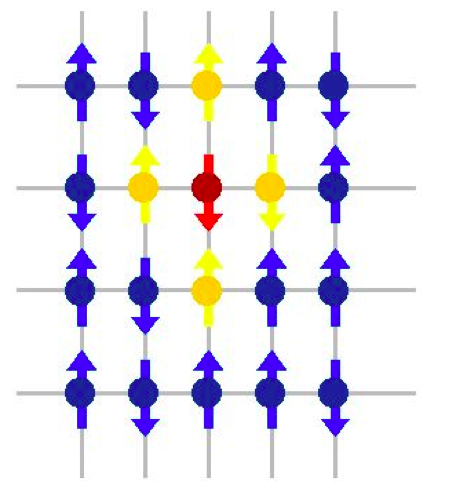
\includegraphics[height=150pt]{pics/ising2}
  \captionof{figure}{Graphical representation of the Ising model on a 2D square lattice.}
  \label{fig:ising}
\end{minipage}%
\hfill
\begin{minipage}{.48\textwidth}
  \centering
  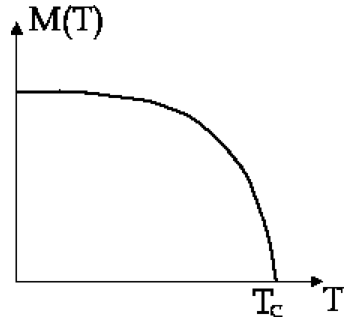
\includegraphics[height=150pt]{pics/spon_mag}
  \captionof{figure}{Spontaneous magnetization in the Ising model.}
  \label{fig:magnetization}
\end{minipage}
\end{minipage}
\vspace{0.1cm}



The simplest approach to the Ising model is imagining a squared lattice and assuming that every variable $\sigma_i \in \mkl{1,-1}$ on the lattice only affects the nearest neighbors (see Fig. \ref{fig:ising}). This restriction can be relaxed by letting the sites interact with the next nearest neighbors or even farther sites. If we think of the variables as spins, their interaction is given by the Hamiltonian 
\begin{equation}
\mathcal{H}\kl{X}=\underbrace{-J\sum_{i,j:\text{nn}}{\sigma_i\sigma_j}}_{A}\underbrace{-H\sum_{i=1}^N{\sigma_i}}_{B}.
\label{eq:hamiltonian}
\end{equation} where A is the interaction between all the nearest neighbors (nn), and B the interaction of each site with an external magnetic field $H$. Note that if two spins are parallel, then the energy is lowered ($-J$) and if they are anti-parallel the energy is increased ($+J$). 



The first term in Eq. \eqref{eq:hamiltonian} tries to create \emph{order} in the system (in the sense of the spins being aligned in the same direction) by reducing the energy when neighboring variables are in the same state. The second term tends to align the spins in the direction of the external field $H$. While the energy is lower in an ordered state, the heat tends to destroy the order by flipping single spins. Beyond a critical temperature $T_c$ (i.e., for  $T>T_c$), the system is dominated by randomness and there is no alignment of the spins anymore. This transition, like any other phase transition (e.g. sol-gel transition) between ordered and disordered states, can be characterized by an \emph{order parameter}. In the case of the Ising model, the order parameter is given by the spontaneous magnetization (see Fig. \ref{fig:magnetization}).


\subsubsection*{The order parameter in the Ising model}
The magnetization is defined as 
\begin{equation}
M\kl{T} =   \avkl{\frac{1}{N} \sum_{i=1}^N{\sigma_i} } ,
\end{equation} that is, the thermal average of the mean value of the spins. This alone would not be  a good measure since taking the thermal average of a quantity means taking the mean value over all the possible states. The problem with this procedure is that for any given state there will always exist an opposite state in which all the spins are flipped. In the average these two configurations cancel each other out. Thus, on average, every state will always cancel out with its opposite companion and the averaged magnetization will always be zero. A better quantity is the \emph{spontaneous magnetization}: 
\begin{equation}
M_\text{S}\kl{T} \equiv \lim_{\vec{H}\rightarrow 0}{  \avkl{\frac{1}{N} \sum_{i=1}^N{\sigma_i} }  }
\label{eq:spon_magn}
\end{equation}
Here the symmetry of the Ising model is broken by applying a small field $\vec{H}$ that aligns the spins in one direction. Now it will not be the same if the spins are up or down, and the thermal average of the spontaneous magnetization won't be zero anymore. Another way of breaking the symmetry would be fixing the boundaries of the lattice in a certain state. This is not practical if periodic boundaries are being used.

In the proximity of the critical temperature, the spontaneous magnetization decays like a power law: 
\begin{equation}
M_\text{S} \propto \kl{T-T_c}^\beta,
\label{eq:powerlaw_unfortunate}
\end{equation}
where $\beta$ is known analytically in 2D (1/8), and numerically in 3D ($\approx 0.326$) (See Fig. \ref{fig:magnetization}).

\subsubsection*{Response functions:}
Response functions are second derivatives of the free energy\footnote{The following established nomenclature is unfortunate: with $\beta$, the thermodynamical quantity $\frac{1}{k_BT}$ is meant, not the exponent presented in the power law \eqref{eq:powerlaw_unfortunate}. See classical statistical physics textbooks for more information.} $E_f = -\frac{1}{\beta} ln \kl{Z}$:

\begin{equation}
\chi\kl{T} \equiv \pder{M}{H}\bigg| _{T,H=0} \propto \abs{T-T_c}^{-\gamma}
\label{eq:susce}
\end{equation}
\begin{equation}
C_{\text{V}}\kl{T} \equiv \pder{E}{T}\bigg| _{H=0} \propto \abs{T-T_c}^{-\alpha}
\end{equation}
The divergence of these functions at the critical temperature can be used to determine the critical temperature itself. We will encounter these functions again later in the context of the $n^{th}$ \emph{order transition} (see Sec. \ref{subsec:first_order_trans}).


\subsubsection*{Fluctuation-dissipation theorem for the magnetic susceptibility:}
Taking equation \eqref{eq:spon_magn}, and plugging it into Eq. \eqref{eq:susce} yields
\begin{equation*}
\chi \kl{T}   =
 \left.\pder{\avkl{M\kl{T,H}}}{H} \right|_{H=0} =
  \pder{}{H} \left.\frac { \sum_X{\sum_{i=1}^N{\sigma_i \exp\ekl{H_0+\beta H \sum_{i=1}^N{\sigma_i}}}}}   {\underbrace   {\sum_X{ \exp\ekl{H_0+\beta H \sum_{i=1}^N{\sigma_i}}}}_{= Z_T\kl{H}}}\right|_{H=0}
\end{equation*}
with $\beta = \frac{1}{k_BT}$ and $H_0=\beta J \sum_{i,j:nn}{\sigma_i\sigma_j}$. Using the product rule yields:
  

\begin{align*}
\chi \kl{T}   &=  \left. \underbrace{\frac   {\beta \sum_X{\kl{\sum_{i=1}^N{\sigma_i} }}^2  \exp\ekl{H_0+\beta H \sum_{i=1}^N{\sigma_i}}  }     {Z_T\kl{H}} }  
-
 \underbrace{\frac   {\beta\kl{ \sum_X{\sum_{i=1}^N{\sigma_i} }  \exp\ekl{H_0+\beta H \sum_{i=1}^N{\sigma_i}} }^2 }    { \kl{Z_T\kl{H}}^2 }} \right| _{H=0}  \\
&=  \hspace{2.4cm} \beta  \avkl{M\kl{T}^2} \hspace{2.7cm} -\hspace{2.6cm}\beta\avkl{M\kl{T}}^2   
\end{align*}
\begin{equation}
\hspace{-7.5cm}=\beta\ekl{ \avkl{M\kl{T}^2}  -  \avkl{M\kl{T}}^2    }\ge 0 \hfill
\end{equation}

\vspace{0.2cm}
and analogously one can show that

\begin{equation}
C_\text{V}=\beta^2 \ekl{    \avkl{E\kl{T}^2}  -\avkl{E\kl{T}}^2  } 
\end{equation} 


You may have already noticed that these expressions are suspiciously similar to the classical definition of the variance. These two last formulae are both very important in Monte Carlo simulations, as we will learn further on.  See Fig. \ref{fig:susce}, \ref{fig:spec_heat}, and \ref{fig:corr_len}.
In the vicinity of $T_c$ (see Fig. \ref{fig:susce}), the magnetic susceptibility decays like a power law: 
\begin{equation*}
\chi \kl{T} \propto \abs{T-T_c}^{-\gamma}
\end{equation*}
with $\gamma$ =7/4 in 2D and $\approx 1.24$ ind 3D.  Near $T_c$ (see Fig. \ref{fig:spec_heat}), the specific heat can also be described by a power law:
\begin{equation*}
C_\nu \kl{T} \propto \abs{T-T_c}^{-\alpha}
\end{equation*}
where the decay is logarithmic in 2D ($\alpha$= 0) and numerically known in 3D ($\alpha$$\approx$ 0.11).

\vspace{0.1cm}


\begin{comment}
\begin{figure}
		\centering
        \begin{subfigure}[b]{0.45\textwidth}
                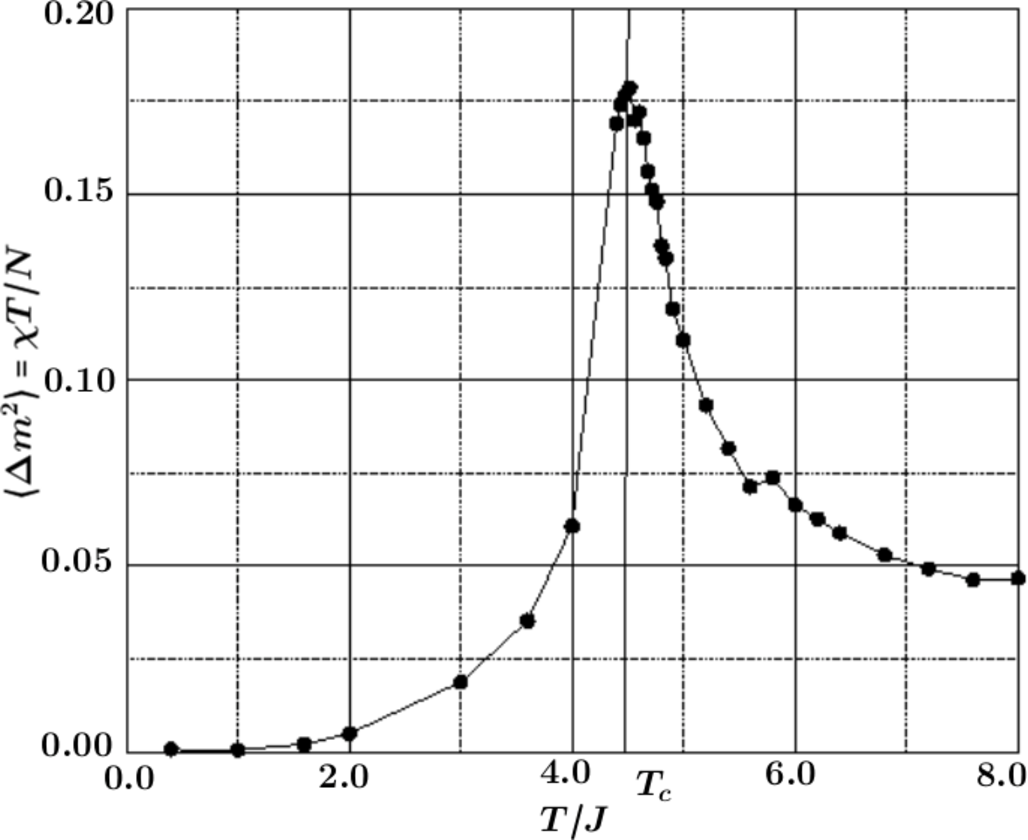
\includegraphics[width=\textwidth]{pics/susce_nottitle.pdf}
                \caption{Susceptibility in a finite system}
                \label{fig:susce}
        \end{subfigure}%
~
       \begin{subfigure}[b]{0.45\textwidth}
                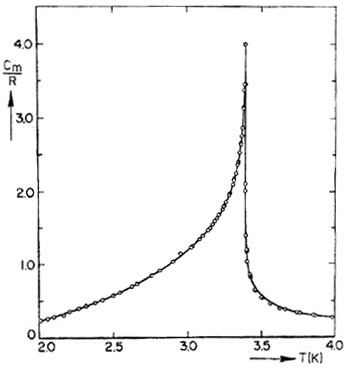
\includegraphics[width=\textwidth]{pics/heat_cap_MIT.jpg}
                \caption{Heat capacity of a binary mixture. Retr. Jan 2015 from web.mit.edu/8.334/www/grades/projects/}
                \label{fig:spec_heat}
        \end{subfigure}
        \caption{Pictures of animals}
	\label{fig:animals}
\end{figure}
\end{comment}



\begin{minipage}{\textwidth}
\begin{minipage}{.5\textwidth}
  \centering
  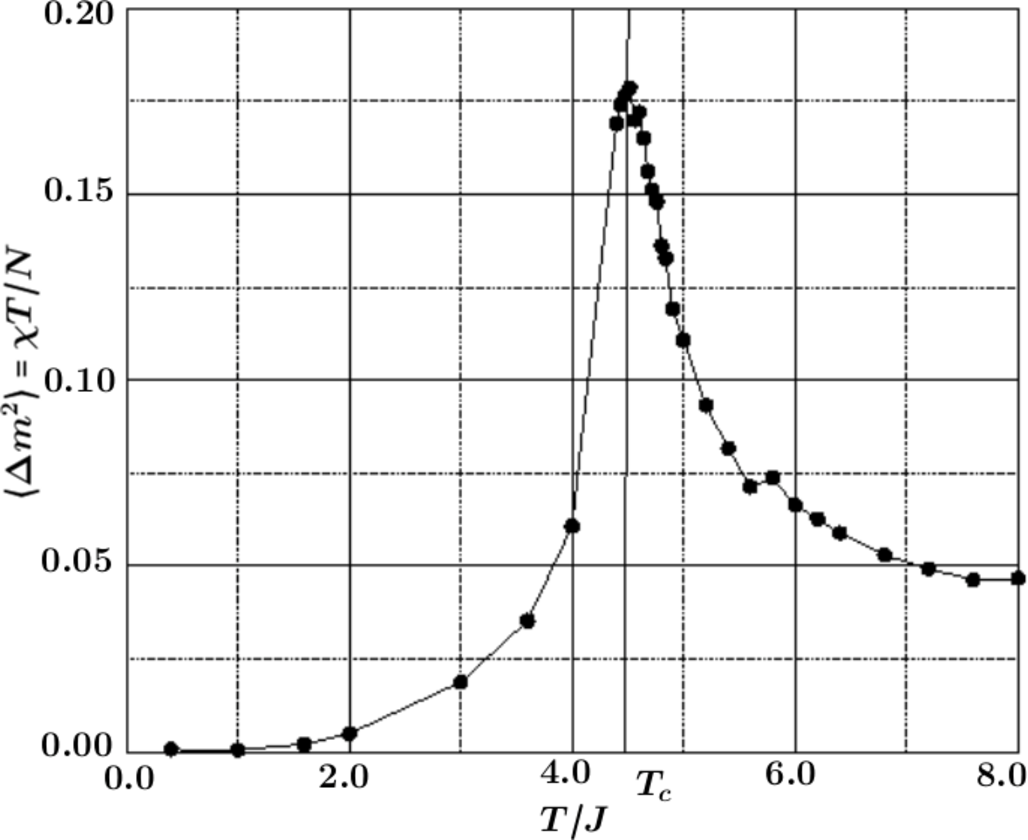
\includegraphics[width=0.95\textwidth]{pics/susce_nottitle.pdf}
  \captionof{figure}{Susceptibility in a finite system}
  \label{fig:susce}
\end{minipage}
\hfill
\begin{minipage}{.5\textwidth}
  \centering
  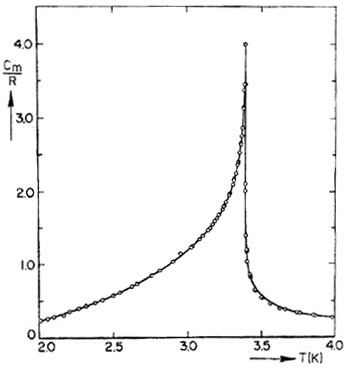
\includegraphics[width=0.95\textwidth]{pics/heat_cap_MIT.jpg}
  \captionof{figure}{Heat capacity of a binary mixture. Retr. Jan 2015 from web.mit.edu/8.334/www/grades/projects/}
  \label{fig:spec_heat}
\end{minipage}
\end{minipage}
\vspace{0.1cm}


\subsubsection*{Correlation length\footnote{See Fig. \ref{fig:corr_len} and the lecture notes \emph{Computational Physics} of the previous course.}}


\begin{wrapfigure}{r}{0.5\textwidth}
  	\begin{center}
    	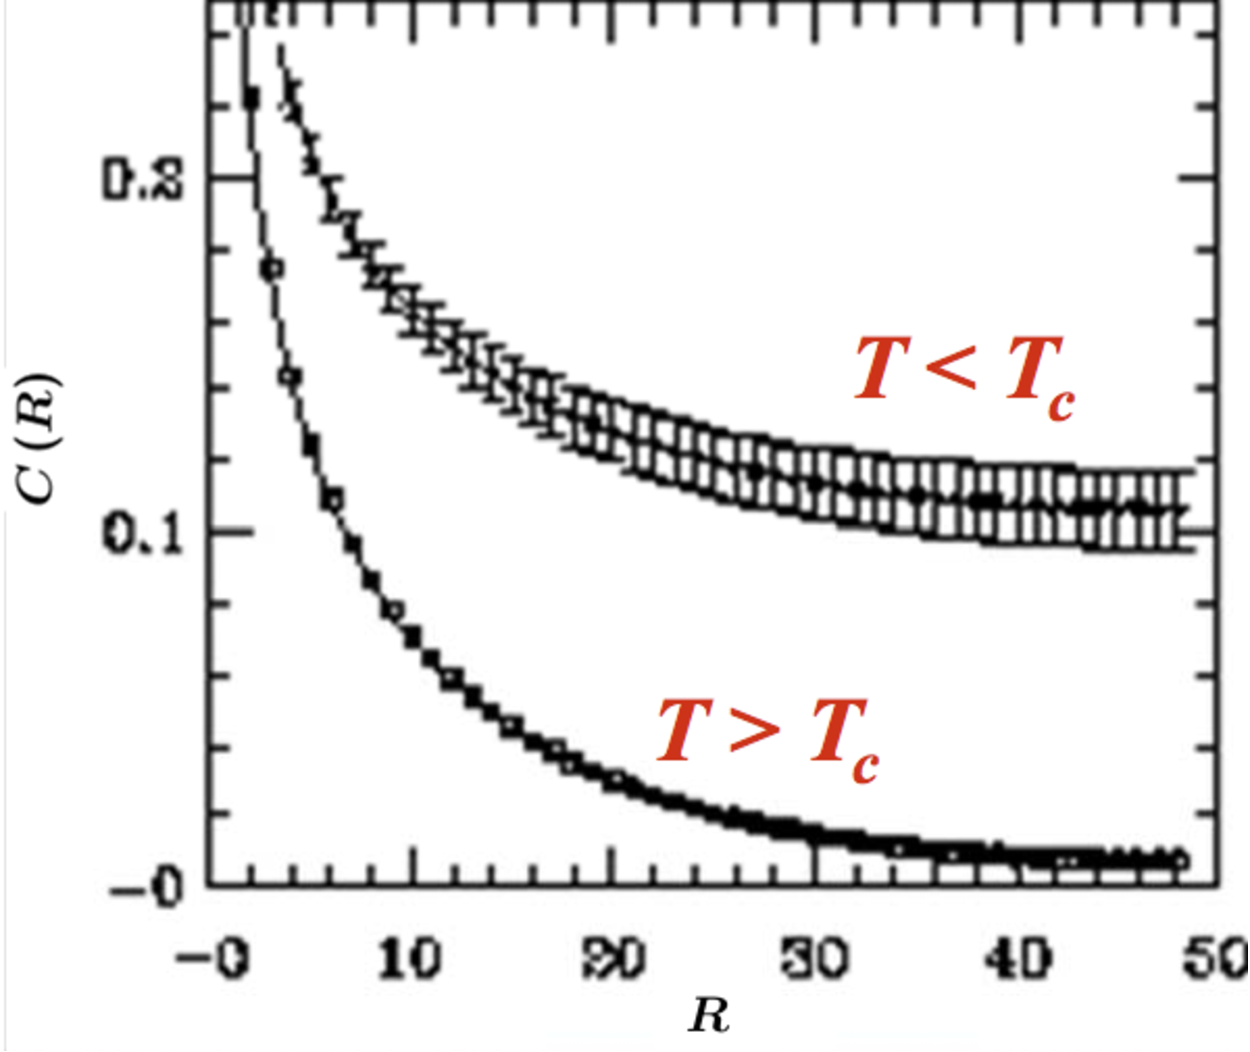
\includegraphics[width=0.4\textwidth]{pics/corr_len.pdf}
		\label{fig:corr_len}
  	\end{center}
  	\caption{Correlation in finite system}
\end{wrapfigure}


The correlation function describes to which extent two sites (or extended regions) are related. It is defined by the thermal average of the product of  the values of sites at different positions:
	\begin{equation}
C(R) \equiv \avkl{\sigma\kl{0}\sigma\kl{R}}.
		\label{eq:corr_len}
	\end{equation}
If two regions are exactly in the same physical state, the correlation function is maximized. This function decays exponentially for large $R$: 
	\begin{equation*}
C(R) \propto M^2 + a e^{-\frac{R}{\xi}}
	\end{equation*}
where $\xi$ is called the \emph{correlation length}.


\begin{comment}
\begin{minipage}{\textwidth}
	\begin{minipage}{.48\textwidth}
The correlation function describes to which extent two sites (or extended regions) are related. It is defined by the thermal average of the product of  the values of sites at different positions:
	\begin{equation}
C(R) \equiv \avkl{\sigma\kl{0}\sigma\kl{R}}.
		\label{eq:corr_len}
	\end{equation}
If two regions are exactly in the same physical state, the correlation function is maximized. This function decays exponentially for large $R$: 
	\begin{equation*}
C(R) \propto M^2 + a e^{-\frac{R}{\xi}}
	\end{equation*}
where $\xi$ is called the \emph{correlation length}.
	\end{minipage}%
	\hfill
	\begin{minipage}{.5\textwidth}
  		\centering
  		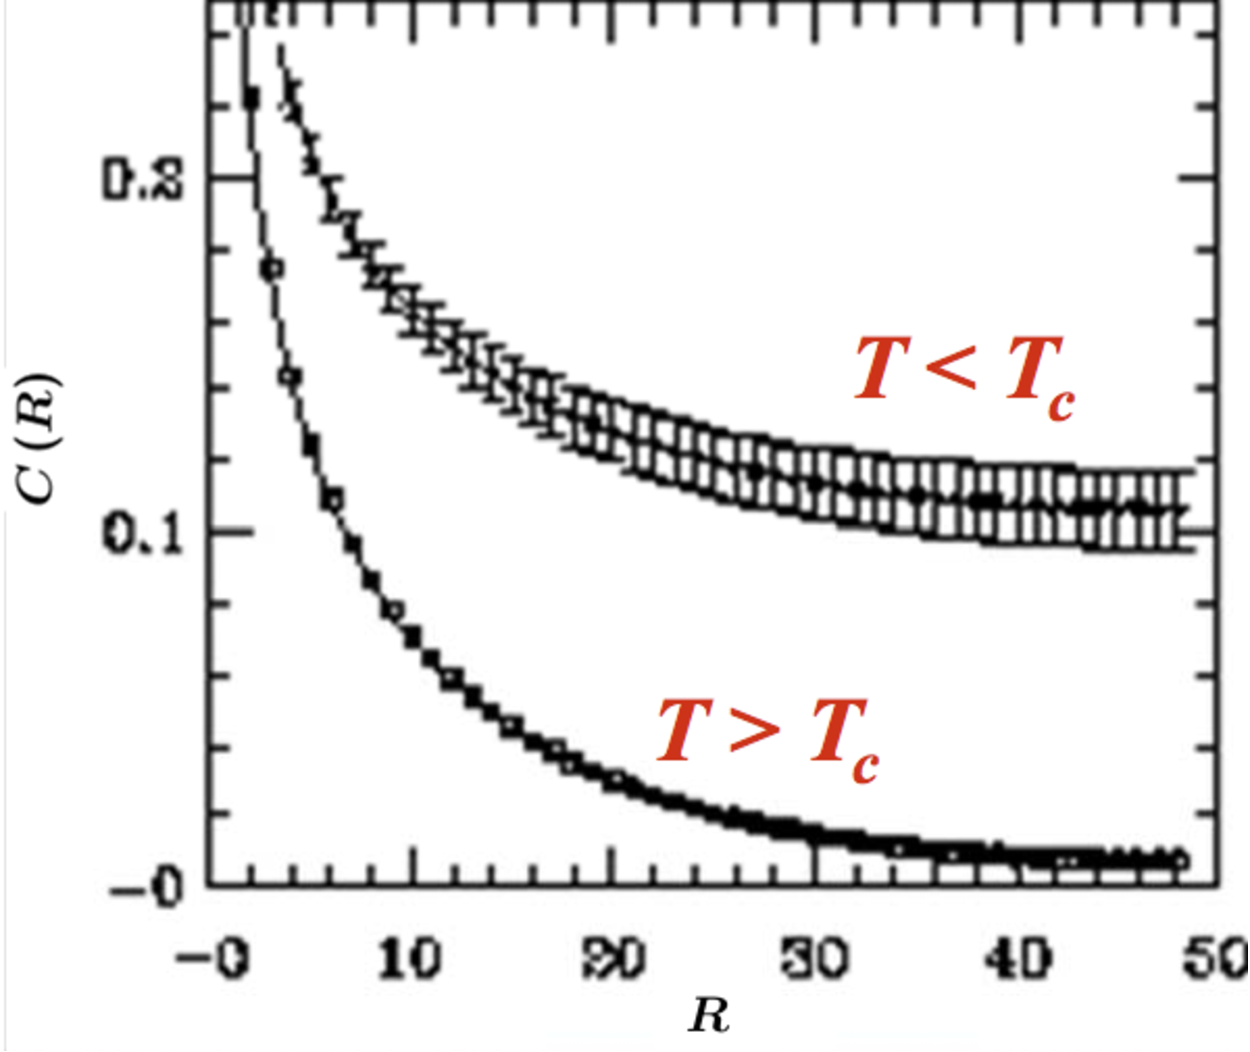
\includegraphics[width=0.95\textwidth]{pics/corr_len.pdf}
  		\captionof{figure}{Correlation in finite system}
  		\label{fig:corr_len}
	\end{minipage}
\end{minipage}
\end{comment}


\vspace{0.1cm}

\noindent
In the vicinity of $T_c$ the correlation length $\xi$ diverges as $$\xi \propto \abs{T-T_c}^{-\nu}$$ with $\nu = 1$ in 2D and $\nu\approx 0.63$ in 3D. At $T_c$ and for large R, we have that $$C(R) \propto R^{2-d-\eta},$$ where d is the dimensionality of the system and $\eta$ = 1/4 in 2D and $\eta\approx0.05$ in 3D.





\subsubsection*{Critical Exponents:}

All the quantities described in Figs. \ref{fig:susce}, \ref{fig:spec_heat} and \ref{fig:corr_len} are characterized by some exponents ($\alpha$, $\beta$, $\gamma$, $\eta$ and $\nu$). An interesting fact is that these exponents are not independent from each other. They are related by the \emph{scaling} and the \emph{hyperscaling} relations \footnote{For more information about these the exponents, see \citet{scaling_stanley} and \citet{stanley}}:

$$\alpha + 2\beta + \gamma =2$$
$$ 2-\alpha =d\nu$$
\begin{equation}(2-\eta)\nu=\gamma\end{equation}
Due to these relations, the number of independent exponents reduces to two.








\section{Monte Carlo Algorithms}

Monte Carlo integration has been already extensively discussed in ICP (see \citep{comp_phys}). In this section, we will briefly summarize how this method works and go deeper into some details and properties we did not study in the past semester. 

\vspace{0.2cm}
\noindent
The basic idea behind Monte Carlo methods is that in order to calculate some thermodynamical quantity, it is enough to sample randomly in phase space instead of averaging over all states. If the sampling is large enough, the computed quantity will eventually converge toward the real thermodynamical quantity. The main steps in the Monte Carlo integration are:

\begin{itemize}
\item Choose randomly a new configuration in phase space (with a Markov chain).
\item Accept or reject the new configuration, depending on the strategy used (e.g., Glauber Dynamics).
\item Calculate the physical quantity and add it in the averaging loop.
\item Repeat the procedure.
\end{itemize}


\subsection{Markov Chains in Monte Carlo: M(RT)$^2$, Glauber, Kawasaki and Creutz algorithms}


\vspace{0.1cm}
\noindent
\begin{minipage}{\textwidth}
\begin{minipage}{.48\textwidth}
Often, choosing equally distributed configurations will be very inefficient since most of the possible configurations are unlikely to be assumed by the system. As an example take the kinetic energy of a gas. The distribution of the average energy will be a sharp peak, as in Fig. \ref{fig:sampling}. There are a number of methods to avoid unnecessary sampling of regions where the system is unlikely to be found (see \emph{importance sampling} in \citet{comp_phys} as an example).
\end{minipage}%
\hfill
\begin{minipage}{.48\textwidth}
  \centering
  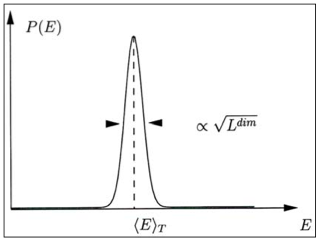
\includegraphics[height=150pt]{pics/sampling}
  \captionof{figure}{Example of energy distribution}
  \label{fig:sampling}
\end{minipage}
\end{minipage}
\vspace{0.1cm}


\begin{comment}


\begin{wrapfigure}{r}{0.5\textwidth}
  	\begin{center}
    	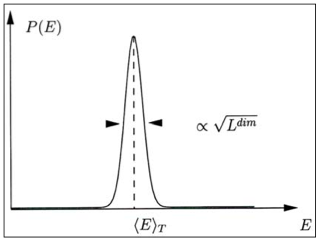
\includegraphics[width=0.5\textwidth]{pics/sampling}
		\label{fig:sampling}
  	\end{center}
  	\caption{Example of energy distribution}
\end{wrapfigure}

Often, choosing equally distributed configurations will be very inefficient since most of the possible configurations are unlikely to be assumed by the system. As an example take the kinetic energy of a gas. The distribution of the average energy will be a sharp peak, as in Fig. \ref{fig:sampling}. There are a number of methods to avoid unnecessary sampling of regions where the system is unlikely to be found (see \emph{importance sampling} in \citet{comp_phys} as an example). 

\end{comment}


A common way to choose the configurations to sample is introducing a virtual time $\tau$ and explore the phase space through a \emph{Markov chain}. Mind that the time $\tau$ has no physical meaning, and it only represents the steps of a stochastic process. 

In terms of a Markov chain, the transition probability from one state to another is given by the probability of a new state to be proposed ($T$) and the probability of this state to be accepted and assumed ($A$). In other words, $T(X\rightarrow Y)$ simply gives us the probability that a new configuration $Y$ is proposed, starting from the configuration $X$. This must fulfill three conditions:
\begin{enumerate}
\item \emph{Ergodicity}: any configuration in the phase space must be reachable within a finite number of steps
\item \emph{Normalization}: $\sum_Y{T(X\rightarrow Y)} =1$
\item \emph{Reversibility}:  $T(X\rightarrow Y)= T(Y\rightarrow X)$
\end{enumerate}
Once a configuration is proposed, one can accept the new configuration with probability $A(X\rightarrow Y)$ or reject it with probability $1- A(X\rightarrow Y)$. The transition probability is then given by
\begin{equation}
W(X\rightarrow Y) = T(X\rightarrow Y) \cdot A(X\rightarrow Y). 
\end{equation}
With the transition probability one can investigate the probability of finding the state in a certain configuration (during the stochastic process, not in real time!) $p\kl{X,\tau}$. The \emph{master equation} describes how the distribution evolves in time. 
\begin{equation}
\der{p\kl{X,\tau}}{\tau}=\sum_Y{p(Y)W(Y\rightarrow X)}  -\sum_Y{p(X)W(X\rightarrow Y) }
\label{eq:master}
\end{equation}
For Markov chains, it is known that the system always reaches a stationary state (called $p_{\text{st}}$) defined by the derivative in Eq. \eqref{eq:master} being zero. The transition probability must fulfill
\begin{enumerate}
\item \emph{Ergodicity}: any configuration must be reachable: $\forall X,Y:$ $W(X\rightarrow Y)\ge0$
\item \emph{Normalization}: $\sum_Y{W(X\rightarrow Y)} =1$
\item \emph{Homogeneity}:  $\sum_Yp_{\text{st}}(Y)W(Y\rightarrow X)= p_{\text{st}}(X)$
\end{enumerate} 
 
Note that the condition of reversibility is not required anymore. This is one of the effects of introducing $A\kl{X\rightarrow Y}$. Just think of a two level system, in which one of the two energy levels is higher (e.g. the electronic shells in an atom): At low energies it would be nonsense to equally sample the excited and the ground state of the electrons. On the contrary, at very high energies the sampling will have to reflect the higher probability of being in an excited state, rather then in the ground state. In order for the Markov chain algorithm to choose effectively which areas of the phase space to explore, somehow $W$ has to depend on the system. Imposing the distribution of the stationary states $p_\text{st}$ as the equilibrium distribution of the physical system $p_\text{st}$ (a real and measurable distribution) is called \emph{detailed balance}:
\begin{equation}
\der{p\kl{X,\tau}}{\tau}=0 \Leftrightarrow p_{\text{st}} \overset{!}{=}  p_{\text{eq}}
\label{eq:detailed_balance}
\end{equation}
It then follows from the stationary state condition ($\der{p\kl{X,\tau}}{\tau}=0$) that
$$\sum_Y{p_{\text{eq}}(Y)W(Y\rightarrow X)}  = \sum_Y{p_{\text{eq}}(X)W(X\rightarrow Y)}.$$ 
A sufficient (not necessary!) condition for this to be true is
 \begin{equation}
 {p_{\text{eq}}(Y)W(Y\rightarrow X)}  = {p_{\text{eq}}(X)W(X\rightarrow Y)}.
 \label{eq:detailed_balance2}
 \end{equation}
As an example, in a canonical ensemble (at fixed Temperature T), the equilibrium distribution is given by the Boltzmann factor: $p_{	\text{eq}}(X)= \frac{1}{Z_T}\text{exp}\ekl{-\frac{E(X)}{k_BT}}$ with the partition function $Z_T=\sum_X{ \text{exp}\ekl{-\frac{E(X)}{k_BT}} }$. The Boltzmann equilibrium indeed fulfills the detailed balance (see M(RT)$^2$ algorithm).




\subsubsection*{M(RT)$^2$ algorithm:}

If equation \eqref{eq:detailed_balance2} is fulfilled, we automatically found the way to fulfill detailed balance by the chosen $W$ and $p_{	\text{eq}}$. The algorithm (also called Metropolis algorithm\footnote{The rather curious name of this algorithm finds its reason in the names of the authors of the paper in which it was proposed: \citet{mrtrt}. \emph{RT} is squared because besides Metropolis, the other four authors of the paper formed two married couples and therefore carried the same family names. The real contributions of some of the authors (in particular of Metropolis and of A.H. Teller) is subject of controversy \citep{controversymrtrt,controversymrtrt2}. It has been even stated by Roy Glauber and Emilio Segr\'e that the original algorithm was invented by Enrico Fermi, which described it to Metropolis while they were working together at Los Alamos and later reinvented by Stan Ulam \citep{segre}.}) uses the acceptance probability 
\begin{equation}
A\kl{X\rightarrow Y} = min\ekl{1,\frac{p_{	\text{eq}}\kl{Y}}{p_{	\text{eq}}\kl{X}}}.
\label{eq:metropolis}
\end{equation}
In the case of the canonical ensemble with $p_{	\text{eq}}\kl{X} = \frac{1}{Z_T}\text{exp}\ekl{-\frac{E(X)}{k_BT}} $ the acceptance probability becomes then
\begin{equation}
A\kl{X\rightarrow Y} = min\ekl{1,\text{exp}\ekl{-\frac{E(Y)-E(X)}{k_BT}} }=min\ekl{1,\text{exp}\ekl{-\frac{\Delta E}{k_BT}} },
\end{equation}
which means that if the energy decreases, the step is always accepted, and if the energy increases it is accepted with probability $\text{exp}\ekl{-\frac{\Delta E}{k_BT}}$. Plugging Eq. \eqref{eq:metropolis} with $p_{	\text{eq}}$ into Eq. \eqref{eq:detailed_balance2} shows that detailed balance is fulfilled. For a more detailed discussion about the Metropolis and alternatives algorithms (e.g. Glauber dynamics), see \citet{comp_phys}. The algorithm has been then generalized in 1970 \citep{mrtrtgeneral}.
We can use this rather general algorithm to explore the phase space of the Ising model, by flipping the values on the lattice following the acceptance probability. Summarized, the steps in the Metropolis algorithm would then be:

\begin{itemize}
\item Choose (randomly) a site $i$
\item Calculate $\Delta E=E(Y)-E(X)=2J\sigma_i h_i$
\item If $\Delta E\leq0$, flip the spin, otherwise accept it with probability $\text{exp}\ekl{-\frac{\Delta E}{k_BT}}$
\end{itemize}
with $h_i=\sum_{i,j:nn}{\sigma_j}$ and $E=-J\sum_{i,j:nn}{\sigma_i\sigma_j}$. Mind that in the case of a squared lattice there are a limited number of possibilities that can occur. Consider creating a look-up table to spare computation time during the acceptance loop. For a 2D lattice, $h_i \in \mkl{0, \pm 2, \pm 4}$.
 
 
 \subsubsection*{Heat bath method (Glauber dynamics):}
The Metropolis algorithm is not the only possible Monte Carlo update: there are a number of other algorithms that fulfill Eq. \eqref{eq:detailed_balance2}. One of these has been elaborated by Glauber, with the acceptance probability given as

 \begin{equation}
A\kl{X\rightarrow Y} \equiv \frac{ \text{exp}\ekl{ - \frac{\Delta E}{k_B T} }}  {    1 + \text{exp}\ekl{ - \frac{\Delta E}{k_B T}}     }
\label{eq:glauber}
\end{equation}

One can see that the expression in Eq. \eqref{eq:glauber} fulfills Eq. \eqref{eq:detailed_balance2}:
 
 
 \begin{align*}
1 &= 1 \\
\Leftrightarrow  \frac{ 1 + \text{exp}\ekl{ - \frac{\Delta E}{k_B T} }  }  {    1 + \text{exp}\ekl{ - \frac{\Delta E}{k_B T}} } &= \text{exp}\ekl{ -\frac{\Delta E}{k_B T} }   \text{exp}\ekl{ +\frac{\Delta E}{k_B T} }  \\
\Leftrightarrow    \frac{ \kl{1 + \text{exp}\ekl{ +\frac{\Delta E}{k_B T}} }\text{exp}\ekl{ - \frac{\Delta E}{k_B T} }}  {    1 + \text{exp}\ekl{ - \frac{\Delta E}{k_B T}}     }  &= \text{exp}\ekl{\frac{ E_X-E_Y}{k_B T} }   \text{exp}\ekl{ +\frac{\Delta E}{k_B T} }   \\
\Leftrightarrow    \kl{1 + \text{exp}\ekl{ +\frac{\Delta E}{k_B T}} }\frac{ \text{exp}\ekl{ - \frac{\Delta E}{k_B T} }}  {    1 + \text{exp}\ekl{ - \frac{\Delta E}{k_B T}}     }  &= \frac{\text{exp}\ekl{\frac{ E_X}{k_B T} }}{\text{exp}\ekl{ \frac{E_Y}{k_B T} } }     \text{exp}\ekl{ +\frac{\Delta E}{k_B T} }   \\
\Leftrightarrow  \text{exp}\ekl{ \frac{E_Y}{k_B T} }    \frac{ \text{exp}\ekl{ - \frac{\Delta E}{k_B T} }}  {    1 + \text{exp}\ekl{ - \frac{\Delta E}{k_B T}}     }  &= \text{exp}\ekl{\frac{ E_X}{k_B T} }    \frac{ \text{exp}\ekl{ +\frac{\Delta E}{k_B T} }}  {    1 + \text{exp}\ekl{ +\frac{\Delta E}{k_B T}}     } \\
\underset{\text{const. temperature}}{\overset{T(X\rightarrow Y)\text{ symmetric}}{\Leftrightarrow}}  {p_{\text{eq}}(Y)T(Y\rightarrow X) A_{Gl.}(Y\rightarrow X)}  &= {p_{	\text{eq}}(X)T(X\rightarrow Y) A_{Gl.}(X\rightarrow Y)}.
\end{align*}
 
 


 
\noindent 
Mind that knowledge about the whole system configuration before the spin flip is not needed here: only the local configuration around the site is relevant. With $J = 1$, the probability to flip the spin $\sigma_i$ is:
$$
A_i = \frac{\text{exp}\ekl{\frac{-2 \sigma_i h_i}{k_BT}}}{1+\text{exp}\ekl{\frac{-2 \sigma_i h_i}{k_BT}}}
$$
with $h_i$ being the local field as usual $h_i = \sum_{j=nn}{\sigma_j}$. Using the abbreviation $p_i \equiv \frac{\text{exp}\ekl{2 \beta h_i}}{1+\text{exp}\ekl{2 \beta h_i}}$, one can express the probability to flip the spin as being

\begin{equation}
p_{\text{flip}} =\begin{cases}
  p_i  & \text{for }\sigma_i=-1\\
  1-p_i & \text{for }\sigma_i=+1
\end{cases}
\text{\hspace{0.5cm} and  \hspace{0.5cm}}\hfill 
p_{\text{no flip}}   =\begin{cases}
  1- p_i  & \text{for }\sigma_i=-1\\
  p_i & \text{for }\sigma_i=+1
\end{cases}
\end{equation}

\noindent
This can be implemented as  $$\sigma_i(\tau+1)=-\sigma_i(\tau)\cdot sign(A_i-z),$$ with $z$ being a random number, or as
$$
\sigma_i(\tau+1) = \begin{cases}
  +1  & \text{with propability }p_i\\
  -1 & \text{with propability }1- p_i
\end{cases}
\text{\hspace{0.5cm} with  \hspace{0.5cm}}\hfill 
p_i \equiv \frac{\text{exp}\ekl{2 \beta h_i}}{1+\text{exp}\ekl{2 \beta h_i}}
$$

This method which does not depend on the spin at time $t$, is called \emph{heat bath MC}.


 
 
\subsubsection*{Binary mixtures (Kawasaki dynamics):}
In this method, the sum of the spins pointing up and the sum of the spins pointing down (i.e., the magnetization) is held constant. Kawasaki dynamics can be used for simulating  binary mixtures of gases and other systems were the population numbers are conserved. In the case of a two species mixture, the energy is larger for A-B bonds, with A and B being the two species in the binary mixture (spin up and spin down particles, two different gas molecules, etc.). What  one can do is to switch two particles with a certain probability and then add the configuration to the averaging loop. 

\subsubsection*{Creutz algorithm:}
Let us consider a situation in which energy is constant. The algorithm generally used in this case is the \emph{Creutz} algorithm. In this technique the condition of energy conservation is relaxed a bit and energy is not exactly conserved anymore. The movement in phase space is therefore not strictly constrained to a subspace of constant energy, but we have a certain additional volume in which we can freely move. The condition is softened by introducing a \emph{demon}, which is a small reservoir of energy $E_d$ that can store a certain maximum energy $E_m$:

\begin{itemize}
\item Choose a site
\item Calculate $\Delta E$ for the spin flip
\item Accept the change if $E_m\ge E_d-\Delta E\ge 0 $
\end{itemize}
This method is completely deterministic (besides the fact that one can randomly choose the sites to update) and therefore reversible. The drawback is that the temperature of the system is not known, but it can be estimated  with the Boltzmann distribution. Taking a histogram of the energies $E_d$ one observes a distribution $P(E_d)\propto \text{exp}\ekl{ -\frac{E_d}{k_BT} }$. The fit is not optimal, since one has very few values of $E_d$. The bigger $E_m$, the faster is the method, since the condition of constant energy is relaxed and the exploration of phase space is less restricted to certain regions. 



\subsubsection*{Q2R:}
In the case of $E_m\rightarrow0$, the Creutz algorithm becomes a totalistic cellular automaton called \emph{Q2R}. The update rules on a square lattice are then given by
 $$
 \sigma_{i,j}(\tau+1) = f(x_{ij})\oplus\sigma_{i,j}(\tau)
 $$
with 
$$
x_{i,j}= \sigma_{i-1,j} +\sigma_{i+1,j} +\sigma_{i,j-1} +\sigma_{i,j+1}
\text{\hspace{0.5cm} and  \hspace{0.5cm}}\hfill 
f(x)=\begin{cases}
  1  & \text{if }x=2\\
  0 & \text{if }x\neq 2
\end{cases}
$$
In this case, the spins are flipped if and only if the change in energy is zero. This can be implemented in a very efficient way using multi spin coding. The changer word defined by $f(x)$ can be expressed in a very elegant way using logical functions:
$$
\sigma(\tau+1) = \sigma(\tau)\oplus\mkl  { \ekl{\kl{\sigma_1\oplus \sigma_2}  \wedge  \kl{\sigma_3\oplus \sigma_4} }  \lor   \ekl{\kl{\sigma_1\oplus \sigma_3}  \wedge  \kl{\sigma_2\oplus \sigma_4} } }
$$
This logical expression can be computed in roughly 12 cycles (8 logical operation and 4 fetches) which last typically around $10$ns. At this computational speed and using multi spin coding (see Sec. \ref{sec:multi_spin}) one can roughly update 4 sites per nanosecond. The method is extremely fast, deterministic and reversible. The problem is that it is not ergodic, and that it strongly depends on the initial configuration. As an example, try to imagine the development of a small lattice, in which only $\sigma_{2,1}$ and $\sigma_{1,2}$ are equal to +1. In fact, this method is not used in statistical physics but it is useful for other purposes e.g., neuroinformatics or cellular automata.




 \subsection{Boundary conditions:}
 
When simulating a lattice, one of the finite size effects that one has to take into account is that at the boundaries the sites do not have further neighbors. The values there can be fixed (boundary condition) or periodic boundaries can be introduced. Mind that this is not only a question of finite size effects, but it can also correspond to some real physical situation. As an example, think of some zero potential boundary condition while solving the electrostatic potential using finite difference methods\footnote{See \citet{comp_phys}}. In finite lattices following methods can be used:

\begin{itemize}
\item Open boundaries, i.e. no neighbors at the edges of the system.
\item Fixed boundary conditions,
\item and periodic boundaries.
\end{itemize}

If our system is big enough\footnote{\emph{Big} here is not purely arbitrary but it depends on what we want to simulate. A good measure of \emph{big} can be that the edges of the system are uncorrelated. It is clear that this method is useless in \emph{small} lattices.} one identies the two sides of the lattice as being neighbors. ($\sigma_{i,L+1}\equiv\sigma_{i,1}$, and $\sigma_{L+1,j}\equiv\sigma_{1,j}$). Identifying the last element of a row (or column) with the first element of the next row (or column) leads to so called \emph{helical boundary condition}. $\sigma_{i,L+1}\equiv\sigma_{i+1,1}$, therefore one can use only one index $k = i+j(L-1)$ instead of keeping track of two.



\subsection{Sampling Uncorrelated Configurations}
Each time we accept a spin-flip in our sampling chain, a new configuration is generated. The problem is that the new and the previous configurations are strongly correlated, and the error analysis (e.g., the decreasing of the error like $\propto \frac{1}{\sqrt{N}}$) is no longer valid. We have to find a measure to know whether we already are in equilibrium or not and to be sure that we are sampling uncorrelated configurations. The (Monte Carlo) time evolution of a quantity is defined as

\begin{equation}
\avkl{A(\tau)}= \sum_X{p\kl{X,\tau}A\kl{X\kl{\tau}}} \overset{\text{eq.}}{=} \sum_X{p\kl{X,\tau_0}A\kl{X(\tau)}}
\end{equation} 




\vspace{0.1cm}
\noindent
\begin{minipage}{\textwidth}
\begin{minipage}{.48\textwidth}

With the condition expressed in \eqref{eq:master}, we know how the probability distribution $p$ evolves. If we assume that our configuration distribution is not at equilibrium at $\tau = \tau_0$, we can define the \emph{non-linear correlation function}:
\begin{equation}
\Phi_A^{nl}\kl{\tau} = \frac {\avkl{A(\tau)}- \avkl{A(\infty)}}  {\avkl{A(\tau_0)}- \avkl{A(\infty)}}
\end{equation}
This is not a correlation function in the strict sense, but it can be a measure to investigate the correlation of the configurations. 
\end{minipage}%
\hfill
\begin{minipage}{.48\textwidth}
  \centering
  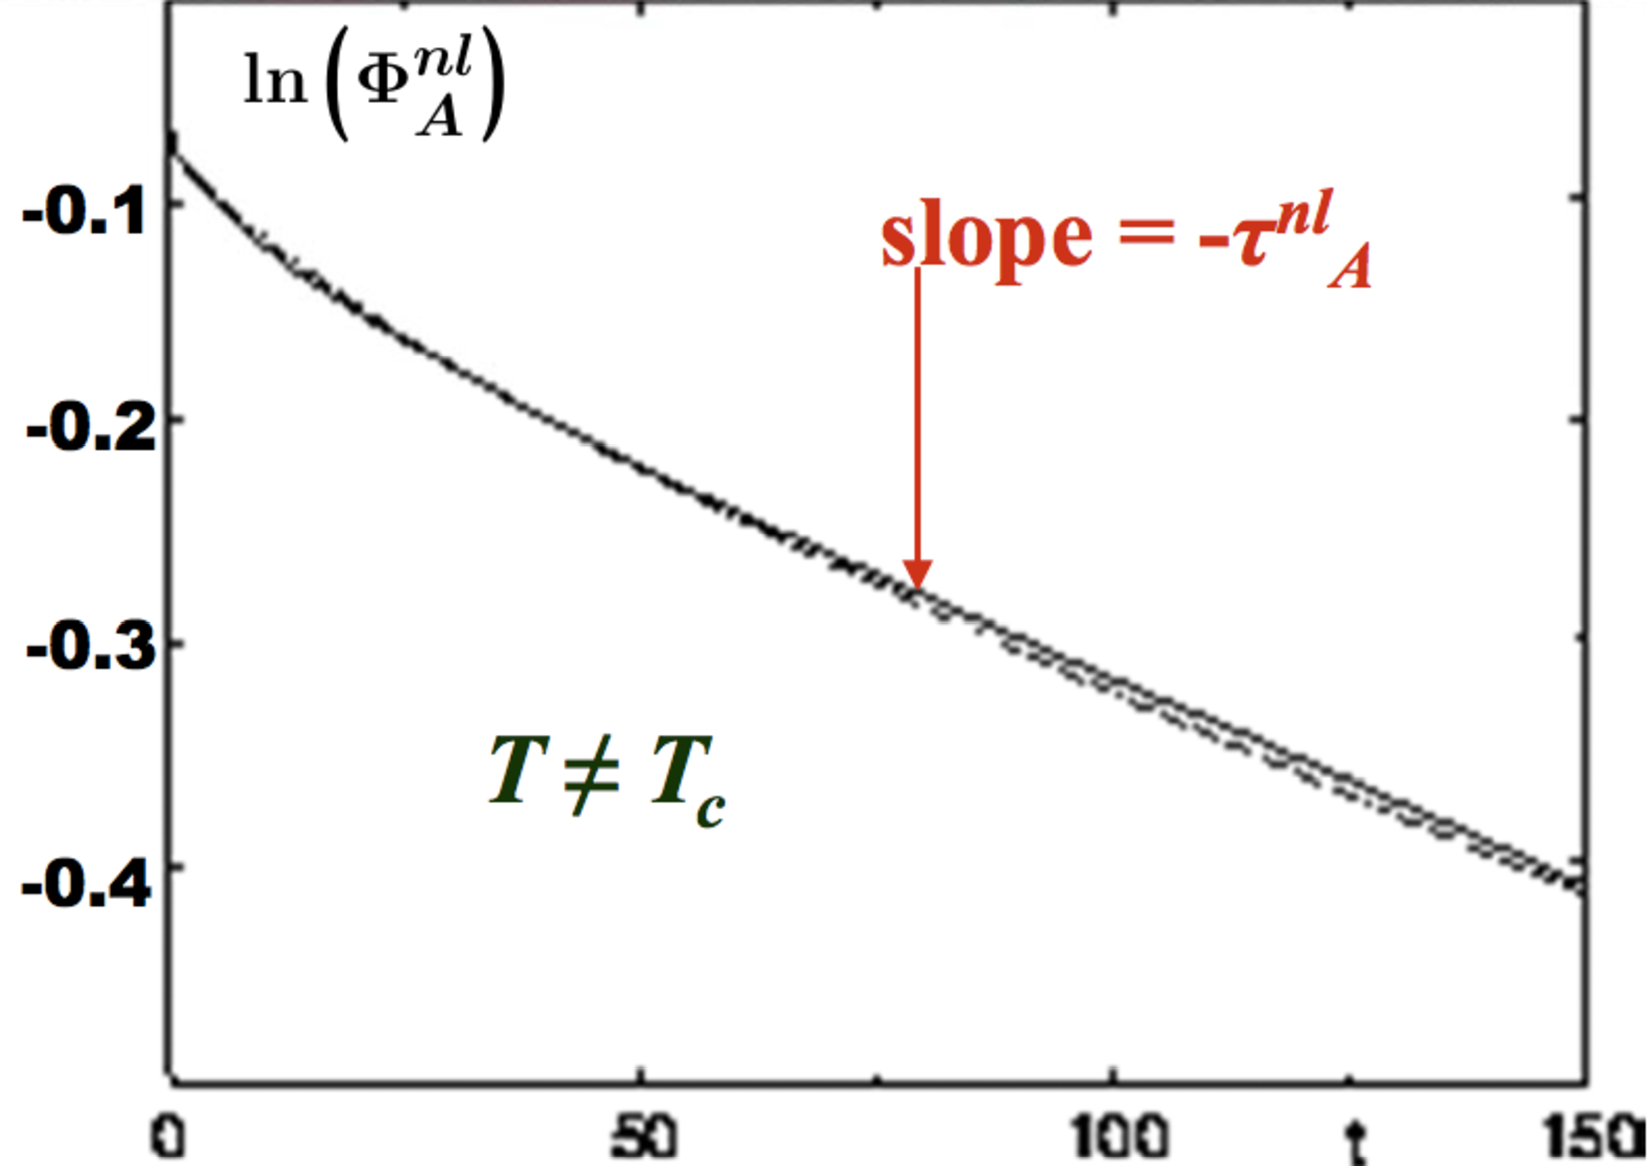
\includegraphics[height=150pt]{pics/non_lin_corr_fun}
  \captionof{figure}{Non-linear correlation function over Monte Carlo time.}
  \label{fig:non_lin_corr_fun.pdf}
\end{minipage}
\end{minipage}
\vspace{0.1cm}



The \emph{non-linear} correlation time $\tau_A^{nl}$ describes the relaxation towards equilibrium:
\begin{equation}
\tau_A^{nl} \equiv \int_0^{\infty} \Phi_A^{nl}\kl{\tau} d\tau
\end{equation}
Near $T_c$, it assumes the form of a power law (\emph{critical slowing down}):
\begin{equation}
\tau_A^{nl} \propto \abs{T-T_c}^{-z_A^{nl}}
\end{equation} with $z_A^{nl}$ being the non-linear dynamical critical exponent. This means that at $T_c$, the time needed to reach equilibrium diverges!






The linear correlation function of two values $A$, $B$
\begin{equation}
\Phi_{AB}\kl{\tau} = \frac {\avkl{A(\tau_0)B(\tau)}- \avkl{A}\avkl{B}}  {\avkl{A B}- \avkl{A}\avkl{B}}
\label{eq:lin_corr_fun}
\end{equation} with $$ \avkl{A\kl{\tau_0} B\kl{\tau}}     =  \sum_X{   p\kl{X,\tau_0} A\kl{X\kl{\tau_0}} B \kl{X\kl{\tau}}     }$$
is now a proper correlation function. Note that it goes from 1 to 0 when $\tau$ goes to infinity. If $A=B$, we call Eq. \eqref{eq:lin_corr_fun} the \emph{autocorrelation function}. For the spin-spin correlation in the Ising model we get:

$$\Phi_{\sigma}\kl{\tau} = \frac {\avkl{\sigma(\tau_0)\sigma(\tau)}- \avkl{\sigma(\tau_0)}^2} {\avkl{\sigma^2(\tau_0)}- \avkl{\sigma(\tau_0)}^2}$$

The \emph{linear} correlation time $\tau_A^{nl}$ describes the relaxation in equilibrium:
\begin{equation}
\tau_{AB} \equiv \int_0^{\infty} \Phi_{AB}\kl{\tau} d\tau
\end{equation}

  \begin{center}
  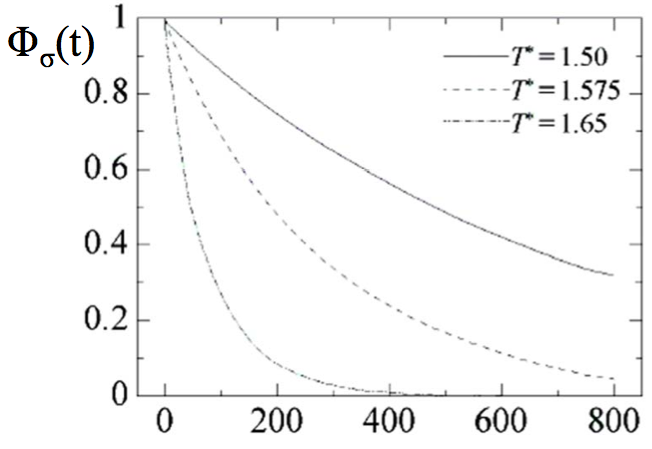
\includegraphics[width=0.7\textwidth]{pics/spin_spin_fun}
  \captionof{figure}{Spin-spin autocorrelation function over MC time in the Ising model.}
  \label{fig:spin_spin_fun}
\end{center}

\begin{comment}

\vspace{0.1cm}
\noindent
\begin{minipage}{\textwidth}
\begin{minipage}{.48\textwidth}
\noindent
If $A=B$, we call Eq. \eqref{eq:lin_corr_fun} the \emph{autocorrelation function}. For the spin-spin correlation in the Ising model we get:

$$\Phi_{\sigma}\kl{\tau} = \frac {\avkl{\sigma(\tau_0)\sigma(\tau)}- \avkl{\sigma(\tau_0)}^2} {\avkl{\sigma^2(\tau_0)}- \avkl{\sigma(\tau_0)}^2}$$

\end{minipage}%
\hfill
\begin{minipage}{.48\textwidth}
  \centering
  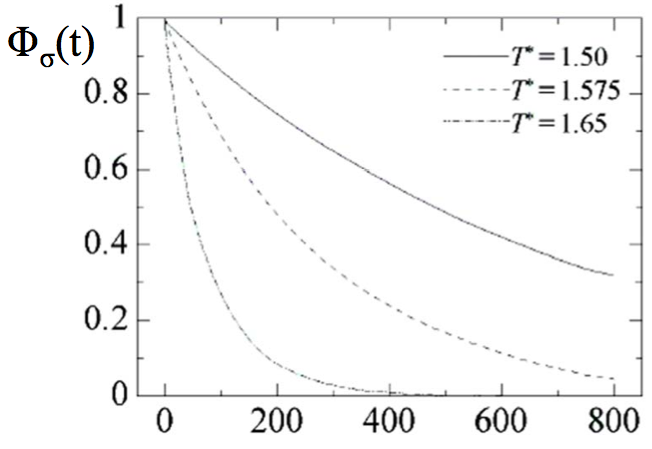
\includegraphics[height=150pt]{pics/spin_spin_fun}
  \captionof{figure}{Spin-spin autocorrelation function over MC time in the Ising model.}
  \label{fig:spin_spin_fun}
\end{minipage}
\end{minipage}
\vspace{0.1cm}

\end{comment}



Near $T_c$, it assumes the form of a power law (\emph{critical slowing down}):
\begin{equation}
\tau_{AB} \propto \abs{T-T_c}^{-z_A}
\end{equation} with $z_A$ being the \emph{linear} dynamical critical exponent.




The dynamical exponents turn out to be 
$$z_\sigma = 2.16 \text{ (in 2D)}$$ $$z_\sigma = 2.09 \text{ (in 3D)}$$ There is a conjectured relation between the critical exponents of the previous sections and the critical dynamical exponents (for spin and for energy correlation) that is numerically well established but not yet analytically proven:

\begin{align}
z_\sigma - z_\sigma^{nl} &= \beta \\ 
z_E - z_E^{nl} &=1- \alpha\\
\end{align}


\subsubsection*{Decorrelated configurations:}


\vspace{0.1cm}
\noindent
\begin{minipage}{\textwidth}
\begin{minipage}{.48\textwidth}
\noindent

The behavior we studied until now is only valid in the case of an infinite lattice. In a finite system there is no divergence by definition (See \citet{comp_phys}). The correlation length diverges at the critical temperature $T_c$:
\begin{equation}
L=\xi\kl{T}\propto \abs{T-T_c}^{-\nu}
\label{eq:corr_len_div}
\end{equation}
$$\Rightarrow \tau_{AB} \propto \abs{T-T_c}^{-z_{AB}}\propto L^{\frac{z_{AB}}{\nu}} $$ 
which means that with growing system size, the number of samples to be discarded also increases.


\end{minipage}%
\hfill
\begin{minipage}{.48\textwidth}
  \centering
  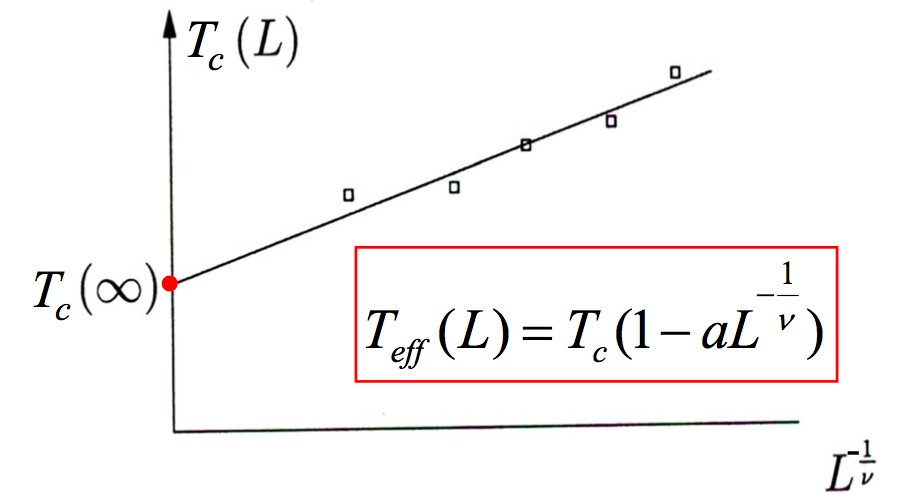
\includegraphics[height=150pt]{pics/finite_size}
  \captionof{figure}{Finite size effects for different system sizes can be used to obtain the critical temperature by extrapolation. See \citet{comp_phys}}
  \label{fig:finite_size}
\end{minipage}
\end{minipage}
\vspace{0.1cm}

\noindent
This is a problem when sampling big systems since the computation becomes very expensive. To be sure not to sample correlated configurations one should 
\begin{itemize}
\item reach equilibrium first  (discard $n_0 = c \tau^{nl}(T)$ configurations).
\item Sample every $n_e^{th}=c \tau(T)$ configurations.
\item At $T_c$ use $n_0 = c L^{\frac{z^{nl}}{\nu}}$ and $n_e=c L^{\frac{z}{\nu}}$
\end{itemize}
where $c \approx 3$ is a "safety factor" to make be sure to discard enough samples. A trick for reducing this effect is using cluster algorithms, which we will encounter later on.




\section{Finite Size Methods}

In the Ising model spins tend to form clusters, which adds a spatial correlation to the time correlation. Quantities already introduced in \citet{comp_phys} and \eqref{eq:corr_len} (the \emph{correlation} and the \emph{correlation length}) are measures for how the system is spatially correlated at separated locations. With increasing distance the correlation decays exponentially until the cut-off due to the finite system size. At $T_c$ the correlation length diverges with an exponent of $-\nu$, as described in Eq. \eqref{eq:corr_len_div}. Many quantities diverge at $T_c$ (e.g. the magnetic susceptibility or the heat capacity). The larger the system size, the more pronounced is the divergence. 


\vspace{0.1cm}
\noindent
\noindent\begin{minipage}{\textwidth}
\begin{minipage}{.5\textwidth}
\noindent
In finite systems there is no real divergence, and the peak will be cut at some value. The maximum of the cutoff in the susceptibility grows proportionally to $L^{\frac{\gamma}{\nu}}$, while the critical region shrinks as $L^{-\frac{1}{\nu}}$. If we rescale the values for different system sizes (i.e., the axes) accordingly, we will get a data collapse (i.e., all the values fall on one single curve). This can be used to find the critical exponents. One can for example plot 
\begin{equation}\chi\kl{T,L}=L^{\frac{\gamma}{\nu}}\cdot F_{\chi}\ekl{\kl{T-T_c}L^{\frac{1}{\nu}}},
\end{equation}
where $F_{\chi}$ is called \emph{scaling function}. See Figs. \ref{fig:scaled_susce}
\end{minipage}%
\hfill
\begin{minipage}{.48\textwidth}
  \centering
  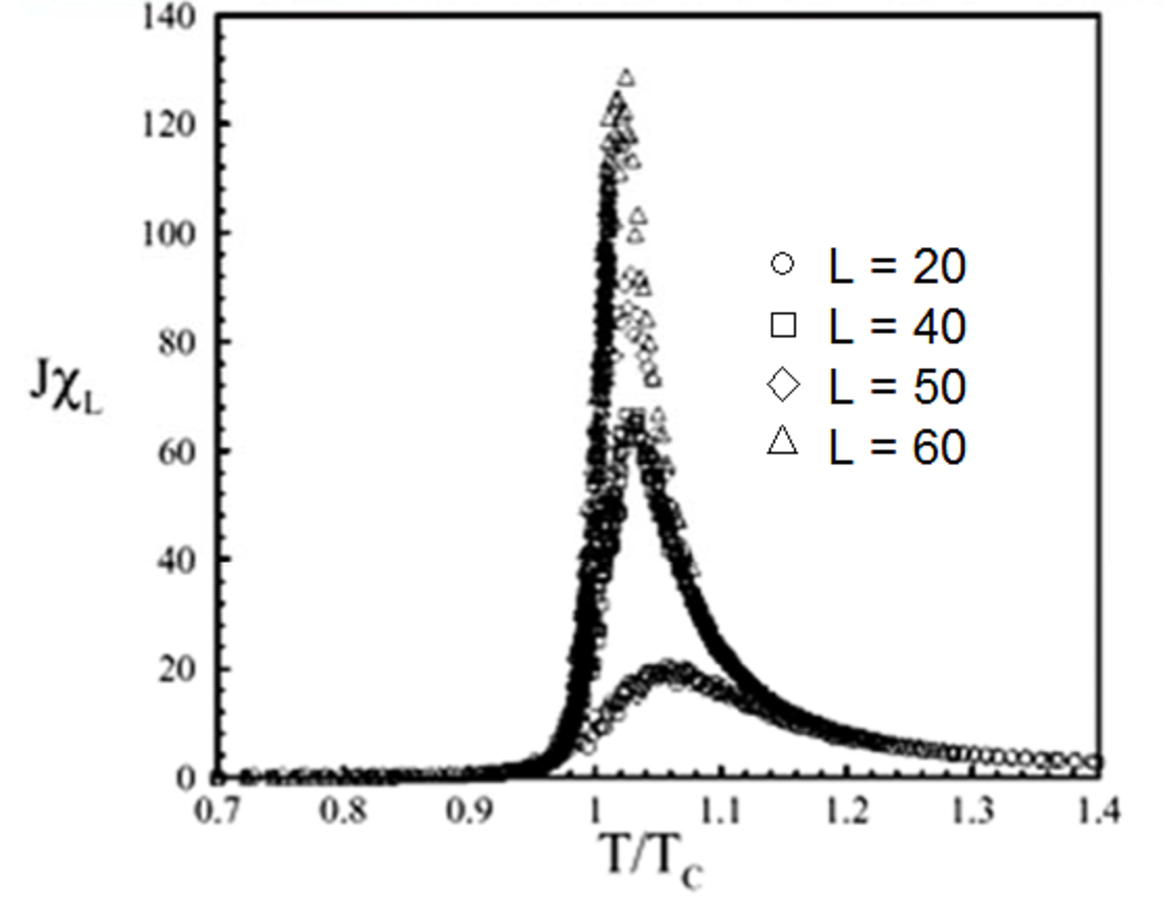
\includegraphics[width=0.9\textwidth]{pics/susce2.pdf}
  \captionof{figure}{Divergence of the magnetic susceptibility for different system sizes. Note that the divergence is more pronounced for larger system sizes.}
  \label{fig:susce2.pdf}
\end{minipage}
\end{minipage}
\vspace{0.1cm}

\subsection{Binder Cumulant}

Binder defined a quantity, which is meant to be independent of the system size L at $T_c$:
\begin{equation}
U_L\equiv 1-\frac{\avkl{M^4}_L}{3\avkl{M^2}^2_L}
\label{eq:bin_cum}
\end{equation}
This can be easily seen:
$$
\frac{\avkl{M^4}_L}{3\avkl{M^2}^2_L} = \frac{L^\frac{4\beta}{\nu} F_{M4}\ekl{\kl{T-T_c}L^\frac{1}{\nu}}}{\kl{L^\frac{2\beta}{\nu} F_{M2}\ekl{\kl{T-T_c}L^\frac{1}{\nu}}}^2} = F_C\ekl{\kl{T-T_c}L^\frac{1}{\nu}}
$$
If $T=T_C$, then the scaling function $F_C$, which is just the ratio of two other scaling functions, is a constant which is independent of the lattice size. For $T>T_C$, the magnetization follows a Gaussian distribution according to 
$$P_L\kl{M}=\sqrt{\frac{L^d}{\pi\sigma_L}}\text{exp}\ekl{-\frac{M^2L^d}{\sigma_L}},
$$ 
with $\sigma_L=k_BT2\chi_L$. Since the fourth moment equals three times the second  moment squared $\kl{\avkl{M^4}=3\avkl{M^2}^2_L}$ it follows that $U_L$ must be zero. Below the critical temperature ($T<T_c$) there are two ground states in the ordered phase (one with positive and one with negative magnetization).
\begin{equation}
P_L\kl{M}=\frac{1}{2}\sqrt{\frac{L^d}{\pi\sigma_l}}\mkl{\text{exp}\ekl{-\frac{\kl{M-M_S}^2L^d}{\sigma_L}}+\text{exp}\ekl{-\frac{\kl{M+M_S}^2L^d}{\sigma_L}}}
\label{eq:dbl_grnd_state}
\end{equation}
For this distribution, it holds that $\avkl{M^4}=\avkl{M^2}^2_L$ and therefore $U_L=\frac{2}{3}$. This means that 
\begin{equation}
U_L =\begin{cases}
  \frac{2}{3} & \text{for }T<T_c\\
  \text{const.} & \text{for }T=T_c\\
 0 & \text{for }T>T_c
\end{cases}
\end{equation}

\vspace{0.1cm}
\noindent
\begin{minipage}{\textwidth}
\begin{minipage}{\textwidth}
This is the most efficient way to calculate the critical temperature, since the Binder cumulant $U_L$ is a quantity which is very sensitive to the temperature. For infinite systems it shows a jump at $T_c$.
\end{minipage}
\begin{minipage}{\textwidth}
  \centering
  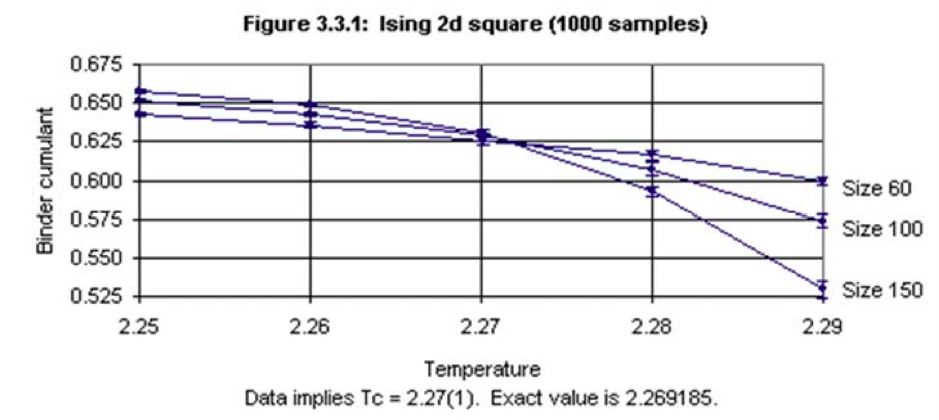
\includegraphics[height=200pt]{pics/bin_cum}
  \captionof{figure}{Binder cumulant for 2D finite systems in the Ising model.}
  \label{fig:bin_cum}
\end{minipage}
\end{minipage}
\vspace{0.1cm}


\vspace{0.1cm}
\noindent
\begin{minipage}{\textwidth}
\begin{minipage}{\textwidth}
The divergence of quantities such as the magnetization, is only approximated as a simple power law. Far away from $T_c$ they do not follow this ansatz anymore, and corrections have to be made. We can observe the subdominant effects of this by calculating the Binder cumulants for small system sizes.
\end{minipage}
\begin{minipage}{\textwidth}
  \centering
  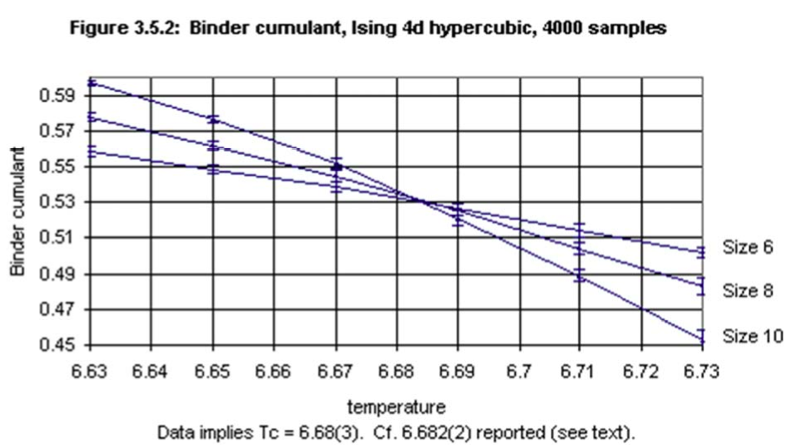
\includegraphics[height=200pt]{pics/bin_cum_4D}
  \captionof{figure}{4D finite systems for the Ising model. Note that the lines do not cross all at the same point.}
  \label{fig:bin_cum2}
\end{minipage}
\end{minipage}
\vspace{0.1cm}

$$M\kl{T} = A_0\kl{T_c-T}^{\beta_0} + A_1\kl{T_c-T}^{\beta_1} + ... $$
$$\xi\kl{T} = C_0\kl{T_c-T}^{\nu_0} + C_1\kl{T_c-T}^{\nu_1} + ... $$
with $\beta_1>\beta$ and $\nu_1<\nu$. These corrections are very important for high quality data, where the errors are small and the deviations become visible. The scaling functions must also be generalized as
$$M\kl{T,L}=
L^{\frac{\beta}{\nu}} F_{M} \ekl{\kl{T-T_c}L^{\frac{1}{\nu}}} +
L^{x} F^1_{M} \ekl{\kl{T-T_c}L^{\frac{1}{\nu}}}+...
$$
with $x=max\ekl{\frac{\beta}{\nu},\frac{\beta}{\nu_1},\frac{\beta}{\nu}-1}$.

\subsection{First Order Transition}
\label{subsec:first_order_trans}

Until now, we only considered critical points for a second order transition, which is characterized by a discontinuity in the second derivative of the free energy (e.g., at the critical temperature). There are also other kinds of transitions, which are characterized by their \emph{order} by means of the $n^{th}$ derivative of the free energy not being continuous. We call those transitions, for which the lowest non-continuous derivative is of order n, $n^{th}$ \emph{order phase transitions}. For $T<T_c$, the Ising model has a jump in the magnetization at $H=0$   (from minus to plus, by varying the field H), which is proportional the first derivative of the free energy. This leads to the susceptibility assuming a delta peak at $H=0$. This kind of phase transition is more common in nature than second order transitions.



\begin{figure}[h!]
		\centering
        \begin{subfigure}[]{0.45\textwidth}
                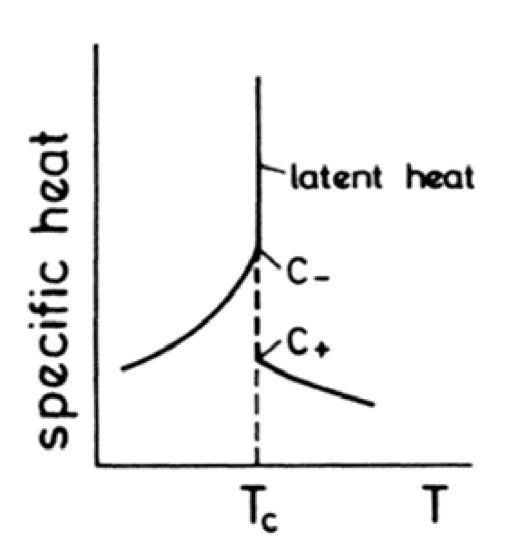
\includegraphics[height=0.9\textwidth]{pics/first_order_heat}
                \caption{Specific heat}
                \label{fig:first_order_heat}
        \end{subfigure}%
~
       \begin{subfigure}[]{0.45\textwidth}
                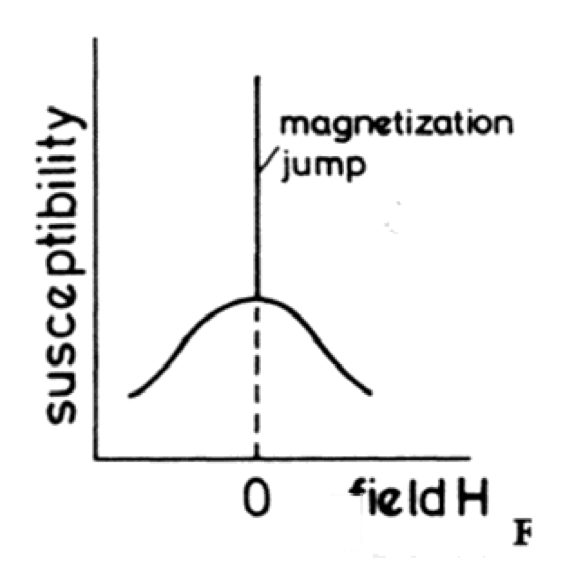
\includegraphics[height=0.85\textwidth]{pics/first_order_magnetization}
                \caption{Susceptibility}
                \label{fig:first_order_magnetization}
        \end{subfigure}
        \caption{First order transitions}
	\label{fig:animals}
\end{figure}


\begin{comment}
\vspace{0.1cm}
\noindent
\begin{minipage}{\textwidth}
\begin{minipage}{.48\textwidth}
  \centering
  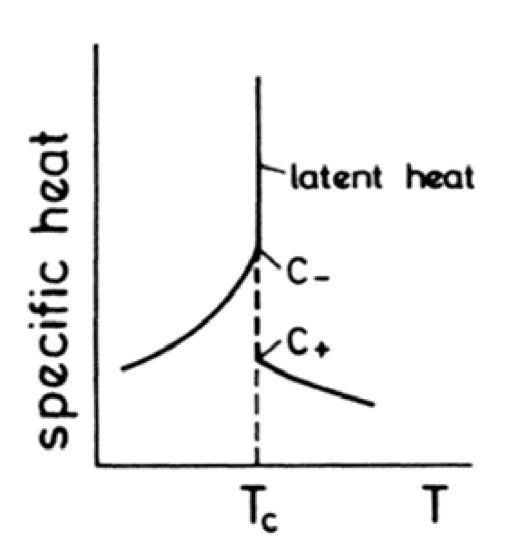
\includegraphics[width=0.9\textwidth]{pics/first_order_heat}
  \captionof{figure}{First order transition manifested in the specific heat.}
  \label{fig:first_order_heat}
\end{minipage}\hfill
\begin{minipage}{.48\textwidth}
  \centering
  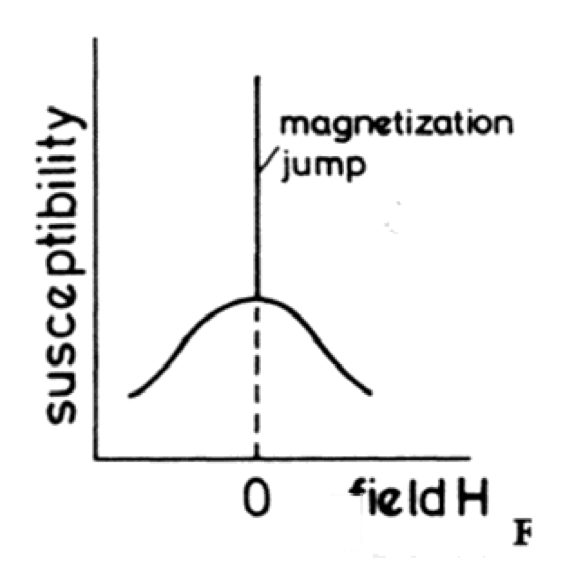
\includegraphics[width=0.9\textwidth]{pics/first_order_magnetization}
  \captionof{figure}{First order transition manifested in the susceptibility.}
  \label{fig:first_order_magnetization}
\end{minipage}
\end{minipage}
\vspace{0.1cm}
%\end{comment}

\noindent
\begin{minipage}{\textwidth}
\begin{minipage}{.38\textwidth}
Usual symptoms of a first order transition are magnetization jumps in small systems (See Fig \ref{fig:magn_jump}), or the hysteresis. In infinite lattices this is not possible since the jump to a ground state of opposite sign would take an infinite (Monte Carlo) time to happen. 
\end{minipage}\hfill
\begin{minipage}{.6\textwidth}
\centering
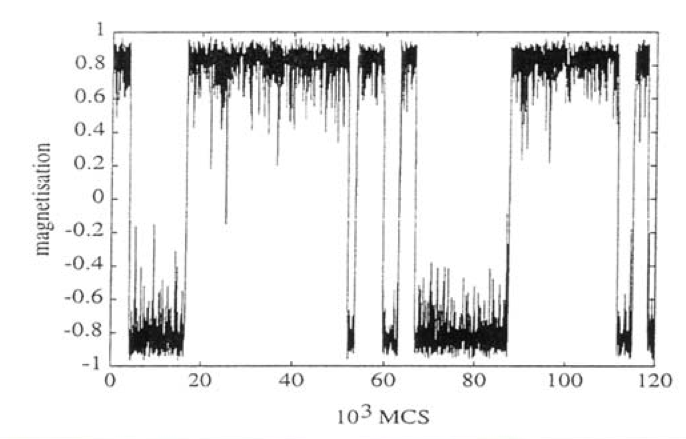
\includegraphics[width=0.95\textwidth]{pics/magn_jump}
\captionof{figure}{First order transitions.}
\label{fig:magn_jump}
\end{minipage}
\end{minipage}

\vspace{0.1cm}

Binder derived that if the distribution of the magnetization is described by two Gaussians, the magnetization (in dependence on the field $H$) has the form of a $\text{tanh}(\alpha L^d)$. Consequently, susceptibility can be calculated by differentiating the magnetization with respect to the field $H$:
\begin{align}
M(H) &= \chi_L^D H + M_L \text{tanh}\kl{\beta H M_L L^d}\\
\chi_L\kl{H} &= \pder{M}{H} = \chi_L^D + \frac{\beta M_L L^d}{\text{cosh}^2\kl{\beta H M_L L^d}}.
\end{align}
Similarly to the scaling for the second order transition, we can scale the maximum of the susceptibility ($\chi_L\kl{H=0}\propto L^d$) and the width of the peak ($\Delta\chi_L\propto L^{-d}$).


\vspace{0.1cm}
\noindent\begin{minipage}{\textwidth}
\begin{minipage}{0.48\textwidth}
  \centering
  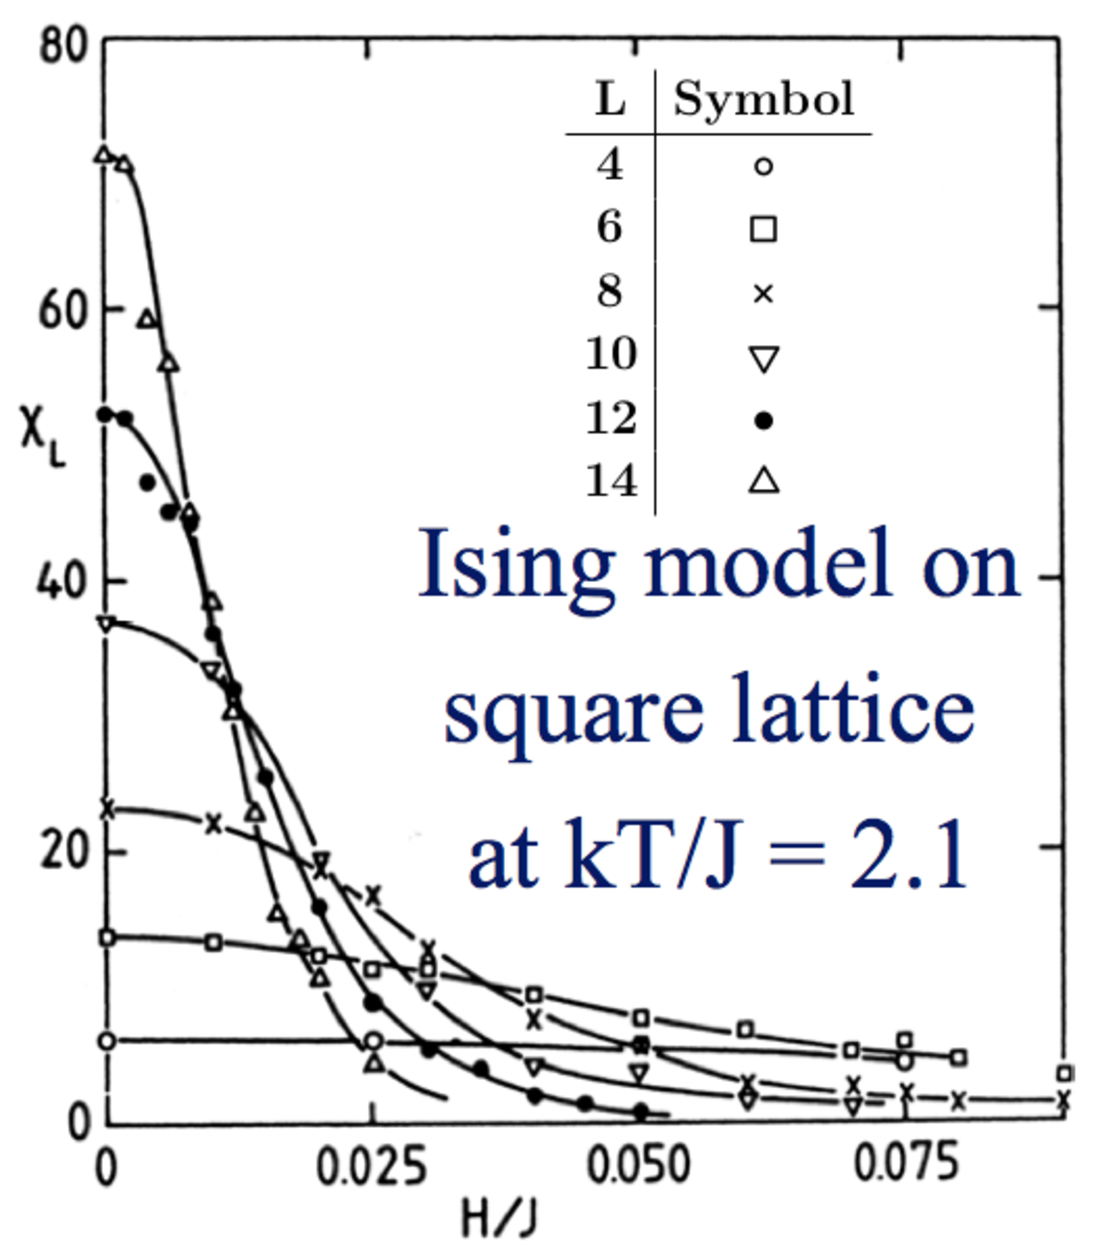
\includegraphics[width=.95\textwidth]{pics/unscaled_susce.pdf}
  \captionof{figure}{Susceptibility for different system sizes in the Ising model.}
  \label{fig:unscaled_susce}
\end{minipage}\hfill
\begin{minipage}{.48\textwidth}
  \centering
  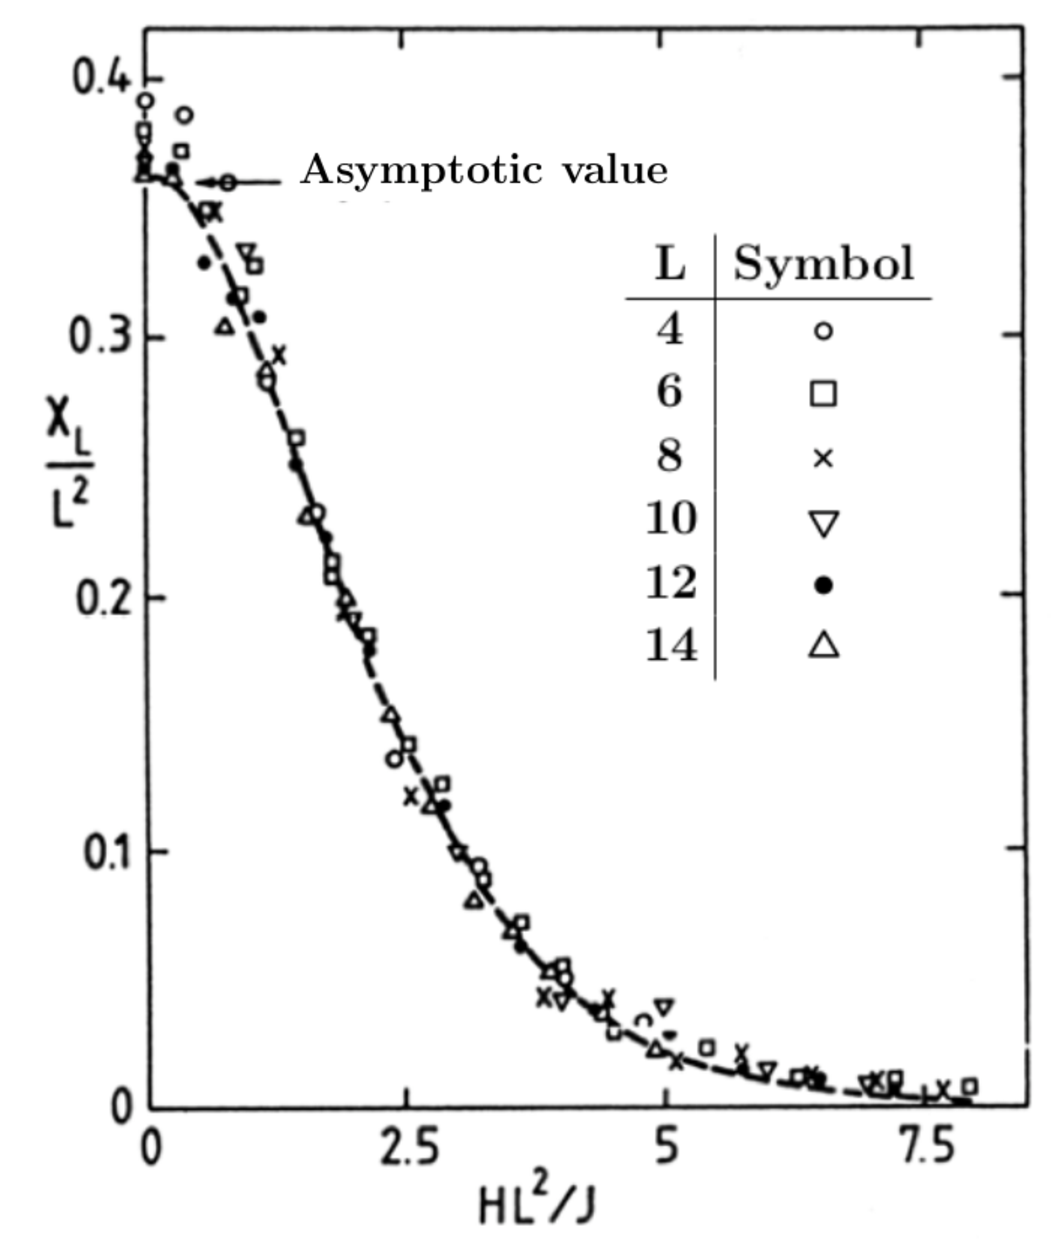
\includegraphics[width=.95\textwidth]{pics/scaled_susce.pdf}
  \captionof{figure}{Data Collapse for scaled susceptibility for different system sizes in the Ising model.}
  \label{fig:scaled_susce}
\end{minipage}
\end{minipage}
\vspace{0.1cm}






\section{Cluster algorithms}
\label{sec:cluster_algorithms}


We have seen that the larger our system is, the longer we have to wait to sample our states. This happened because just flipping one or a few spins before sampling ends up in a strong correlation between the states, and the assumption of statistically independent samples is not given anymore. The aim of cluster algorithms is to reduce this critical slowing down by flipping multiple spins. It is essential that the group of spins to flip is chosen with a tiny acceptance probability. To do this, we will generalize the Ising model and adapt it to our needs.

 
\subsection{Potts Model}
The Potts model is a generalization of the Ising model to a $q$-states model, and it also exhibits in certain cases a first order phase transition at a critical temperature. Applications of the Potts model range from sociology through biology to material science, making this a very versatile model. The Potts model exhibits a first order transition in 2D for any $q$ larger than 4, and for any $q$ larger than 2 for dimensions larger than 2. We start by defining the Hamiltonian of the system as
\begin{equation}
\mathcal{H} = -J\sum_{i,j=nn} \delta_{\sigma_i,\sigma_j} - H_1\sum_{i} \delta_{\sigma_i,\sigma_1}
\label{eq:potts_model}
\end{equation}
with $\sigma_i \in \mkl{1,...,q}$, and $q$ being an integer $\geq 2$. In this case, the state ``1'' is favored, by lowering the energy whenever a site is in this particular state. The sites of the lattice we are dealing with can assume more than just two states (up/down, as we had in the Ising model). The interesting fact now is that there is a strong connection between the Potts model and the well known bond percolation model. After Kasteleyn and Fortuin (1969), which we will discuss now, the two models have related partition functions. 


\vspace{0.1cm}
\noindent
\noindent\begin{minipage}{\textwidth}
\begin{minipage}{.98\textwidth}
  \centering
  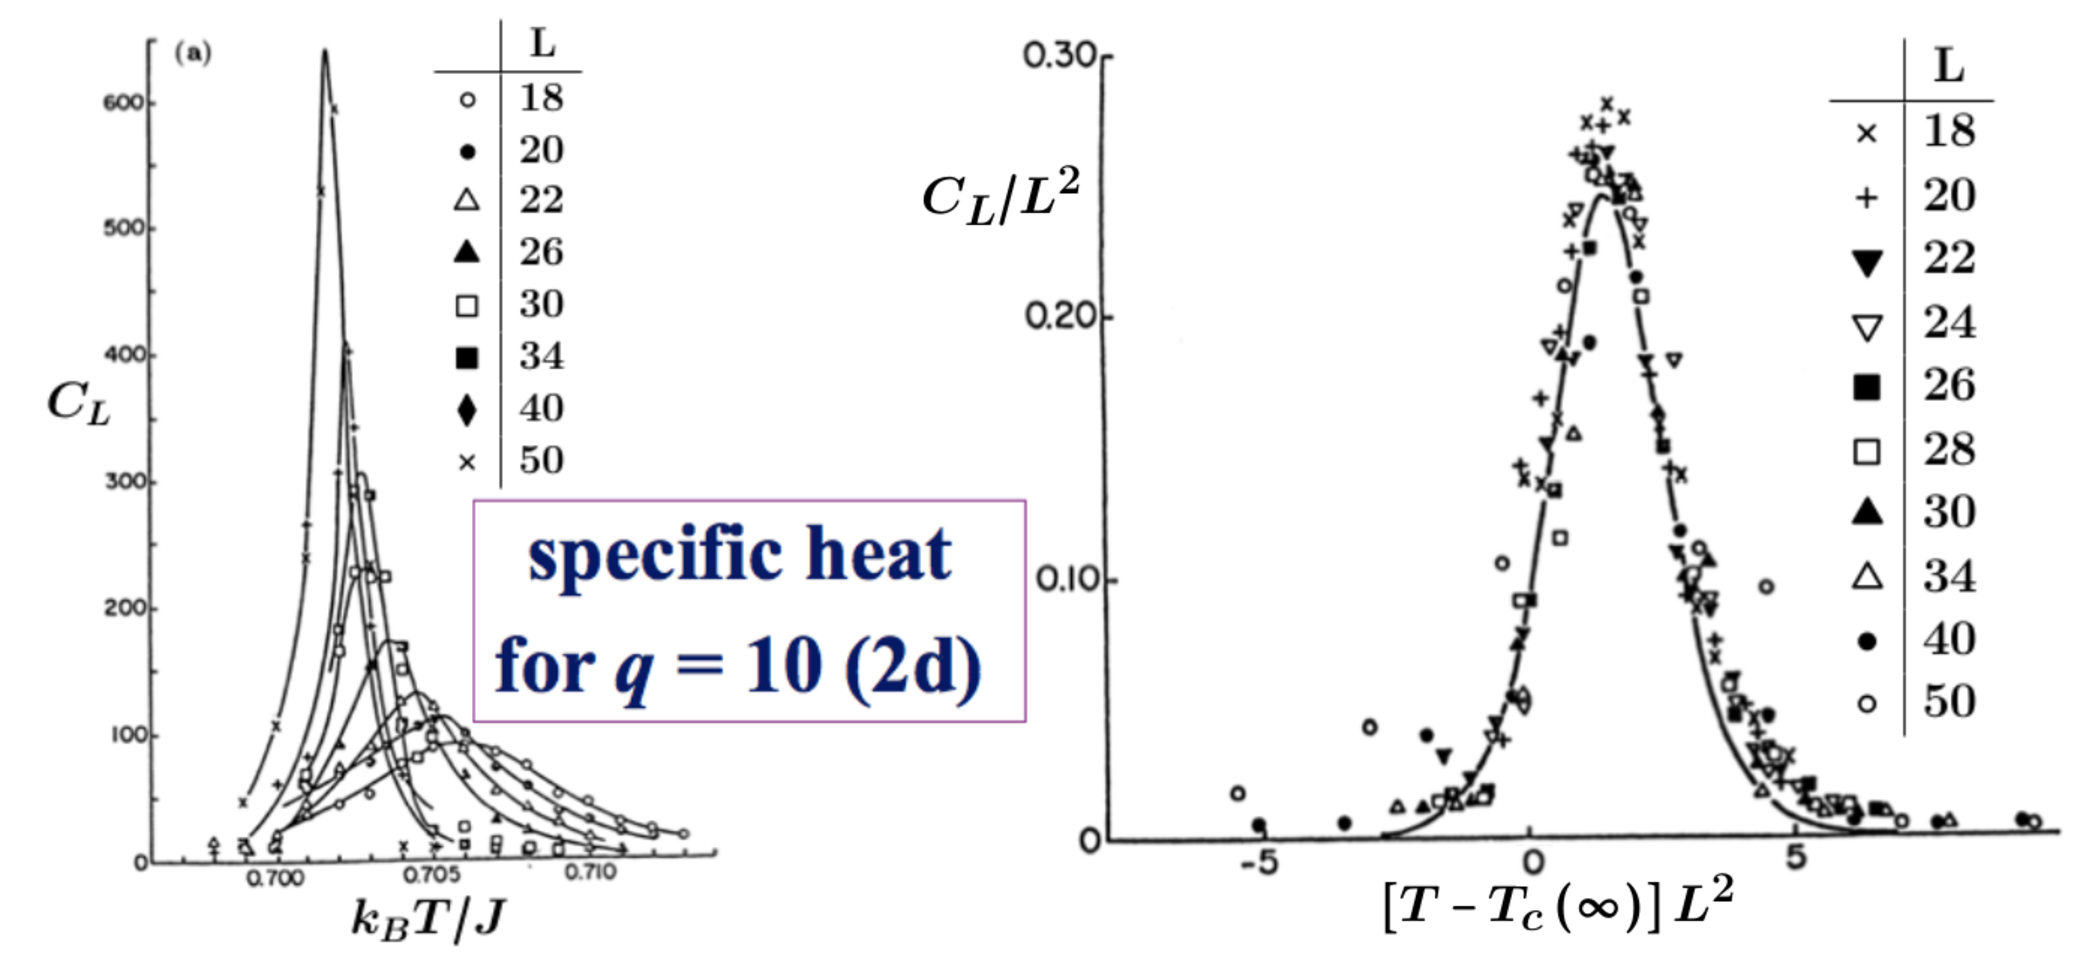
\includegraphics[width = 0.95\textwidth]{pics/potts10}
  \captionof{figure}{Specific heat for two dimensional Potts model with q=10. On the right the scaling for different sizes.}
  \label{fig:potts10}
\end{minipage}\hfill
\end{minipage}
\vspace{0.1cm}

Any system is characterized by its partition function. From the latter one can derive all other thermodynamic quantities. Therefore the complete knowledge of the partition function corresponds to the complete knowledge of the system. If two systems have exactly the same partition function, those two systems are therefore equivalent. In the following, we will prove a relation between the bond percolation and the Potts model.


\subsubsection*{The Kasteleyn and Fortuin theorem:}
Consider the Potts model not on a square lattice, but on an arbitrary graph of nodes connected with bonds. On the nodes we have $q$ possible states, and for every connection we have an energy cost of 1 if two connected nodes are in a different state and of 0 if they are in the same state.
\begin{equation}
E= J \sum_\nu \epsilon_\nu \hspace{1cm} 
\text{with }
\epsilon_\nu =\begin{cases}
  0  & \text{if endpoints are in the same state }\\
  1 & \text{else }
\end{cases}
\label{eq:energy_potts}
\end{equation}

We also introduce two operations on the bonds: the \emph{contraction C} and \emph{deletion D} (see Fig. \ref{fig:contr_del}). Bonds can thus be either removed by merging two sites (which implies that they have the same state) or be simply removed.

  \begin{center}
  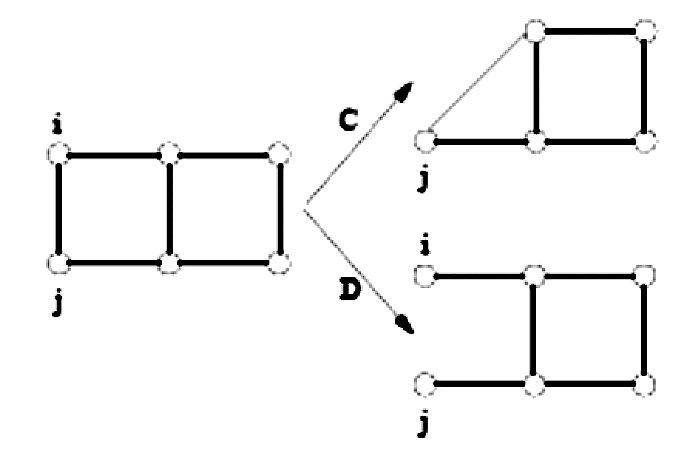
\includegraphics[width = 0.7\textwidth]{pics/contr_del}
  \captionof{figure}{Contraction and deletion of bonds.}
  \label{fig:contr_del}
\end{center}
\vspace{0.1cm}

\begin{comment}
\vspace{0.1cm}
\noindent
\noindent\begin{minipage}{\textwidth}
\begin{minipage}{.48\textwidth}
We also introduce two operations on the bonds: the \emph{contraction C} and \emph{deletion D} (see Fig. \ref{fig:contr_del}). Bonds can thus be either removed by merging two sites (which implies that they have the same state) or be simply removed.
\end{minipage}\hfill
\begin{minipage}{.48\textwidth}
  \centering
  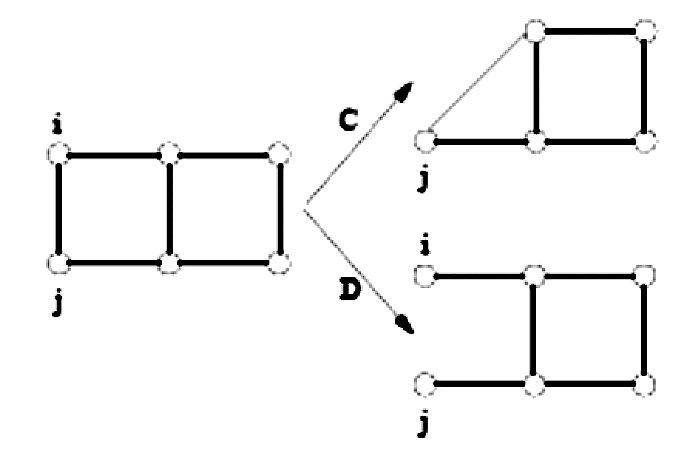
\includegraphics[height=150pt]{pics/contr_del}
  \captionof{figure}{Contraction and deletion of bonds.}
  \label{fig:contr_del}
\end{minipage}
\end{minipage}
\vspace{0.1cm}
\end{comment}

The partition function is the sum over all the possible configurations weighted by the Boltzmann factor:
\begin{equation}
Z=\sum_X{      e^{    -\beta E\kl{X}    }       } 
\overset{\text{\eqref{eq:energy_potts}}}{=} 
\sum_X{e^{-\beta J \sum_\nu {\epsilon_\nu}}} =
\sum_X   \prod_\nu{e^{-\beta J\epsilon_\nu}} 
\end{equation}
We will now consider a particular bond $\nu_1$ and rewrite the partition function as
\begin{align*}
\sum_X  e^{-\beta J\epsilon_{\nu_1}} \prod_{\nu\neq\nu_1}{e^{-\beta J\epsilon_\nu}} &=
\sum_{X,\sigma_i =\sigma_j}  \prod_{\nu\neq\nu_1}{e^{-\beta J\epsilon_\nu}} + e^{-\beta J} \sum_{X,\sigma_i\neq\sigma_j}  \prod_{\nu\neq\nu_1}{e^{-\beta J\epsilon_\nu}} \\
& =Z_C + e^{-\beta J} \kl{Z_D - Z_C}\\
& = \kl{1 - e^{-\beta J\epsilon_\nu}} Z_C + e^{-\beta J}Z_D\\
&= p Z_C + \kl{1-p} Z_D
\end{align*}
Here $\sigma_i$ and $\sigma_j$ are the states at the two ends of the bonds, $Z_C$ and $Z_D$ are the partition functions of the graphs contracted and deleted at $\nu_1$ respectively and $p\equiv1-e^{-\beta J}$ . We have now divided the partition function in a sum of two other partition functions, namely the partition function of the same system with a deleted bond and the partition function of the same system with a contracted bond. We can repeat this operation on another bond $\nu_2$, and we find that
$$
Z = p^2Z_{C_{\nu_1},C_{\nu_2}} + p(1-p) Z_{C_{\nu_1},D_{\nu_2}} + (1-p)^2 Z_{D_{\nu_1},D_{\nu_2}}.
$$
We repeat this operation on every bond. At the end the graph is reduced to a set of separated points corresponding to connected/contracted bonds: the clusters of sites which are connected and in the same state. The partition function is then reduced to:
\begin{equation}
Z= \sum_{\underset{\text{{ bond percolation}}}{\text{ \fontsize{6.5}{4}\selectfont configuration of}}} {q^{\text{\# of clusters}} p^c \kl{1-p}^d}
= \avkl{q^{\text{\# of clusters}}}_{\text{bond percolation configurations}}
\label{eq:part_func_coniglio}
\end{equation}
where $c$ and $d$ are the numbers of contracted and deleted bonds respectively. We have now an equivalence between a purely geometrical model (percolation) and a thermal (or magnetic) model with a Hamiltonian (Potts model). Interestingly, one could now choose values for $q$ which are not integers. This made no sense in the beginning since $q$ was introduced as the state of each site. 

\subsubsection*{Coniglio-Klein clusters:}
Mind that the equivalence between the bond percolation model and the magnetic model is of statistical nature, since a particular bond configuration can have several spin configurations and a particular spin configuration can have several bond configurations. The fact that the value of the spins is absent in Eq. \eqref{eq:part_func_coniglio} forms the base for cluster algorithms. The probability of a given cluster $C$ to be in a certain state $\sigma_0$ is independent of the state itself:
\begin{equation}
p(C,\sigma_0) = p^{c_C}(1-p)^{d_C}  \sum_{\underset{\text{{ without cluster C}}}{\text{ \fontsize{6.5}{4}\selectfont bond percolation}}} {q^{\text{\# of clusters}} p^c \kl{1-p}^d}
\end{equation}

This means that flipping this particular cluster won't affect the partition function (and therefore the energy) so that it is possible to accept the flip with probability one. This can be seen by looking at the detailed balance for this system:
\begin{equation}
p(C,\sigma_1)W\ekl{(C,\sigma_1)\rightarrow (C,\sigma_2)}
=
p(C,\sigma_2)W\ekl{(C,\sigma_2)\rightarrow (C,\sigma_1)}
\end{equation}
and remembering that $p(C,\sigma_1)=p(C,\sigma_2)$. If we now apply Glauber dynamics we obtain $W=\frac{p(C,\sigma_2)}{p(C,\sigma_1)+p(C,\sigma_2)}=\frac{1}{2}$ and  $W=min\ekl{1,\frac{p(C,\sigma_2)}{p(C,\sigma_1)}}=1$ for Metropolis. This makes the cluster algorithm much faster than single-spin flip algorithms and reduces the problem of critical slowing down.

\subsection{O(n) Model}
There are a number of models that resemble the Ising model, but with slight modifications to adapt them to a particular context (e.g., the antiferromagnetic models, Ising spin glass, ANNNI model, metamagnets, ...). One of the possible generalizations of the Ising model is the so called n-vector model. Unlike the Potts model, it takes into account that the degrees of freedom of the sites do not have to be discrete. This is a very important model for describing phenomena related to magnetism (e.g., ferromagnetism). The variables on the sites are n-dimensional vectors. The Hamiltonian resembles the one of the Potts model in the sense that it favors alignment of the variables:

\begin{equation}
\mathcal{H} = J \sum_{i,j: nn} {\vec{S}_i \cdot \vec{S}_j } + H_1\sum_{i} { \vec{S}_i^1} 
\text{  \hspace{0.1cm}  with  \hspace{0.1cm} }
\vec{S}_ i= \kl{S_i^1,S_i^2,...,S_i^n} 
%\text{ \hspace{0.04cm} and  \hspace{0.04cm} }
\text{  and   }
\abs{\vec{S}_ i}= 1
\label{eq:antiferromagnetic}
\end{equation}
For $n=1$ we retrieve the Ising model, for $n=2$ we have the \emph{XY-model}, for $n=3$ the \emph{Heisenberg model} and finally, for $n=\infty$ we have the \emph{spherical model}.

Note that the models for various values of $n$ are not equivalent. In fact, there are huge differences. As an example, the XY-model does not exhibit any phase transition from an ordered to a disordered state. The proof of this statement can be found in \citet{mermin}, and it is known as the Mermin-Wagner theorem. Ernst Ising himself proved in his PhD thesis that the one dimensional case also does not exhibit any phase transition. In three dimensions, however, there are phase transitions and the behavior regarding magnetization, susceptibility and specific heat is very similar to the behavior of the Ising model we studied earlier (critical temperature, critical exponents etc.). 

For Monte Carlo simulations with continuous degrees of freedom we have to adapt our techniques because phase space is not a discrete set of configurations anymore. The classical strategy is to make spin flips by modifying the spin locally by a fixed amount (a rotation): $\vec{S}_i'=\vec{S}_i +\Delta \vec{S} $. The classical Metropolis algorithm can then be used in the same fashion as in the discrete models. In order to use cluster methods one can project a group of spins onto a plane, and then reflect the spins with respect to the plane.

In order to obtain clusters one has to find a method to identify ``equal'' spins. The probability to find equal spins in a continuous model vanishes and one can therefore considers a certain range of values instead(if two spins are equal within a certain error, then they belong to the same cluster).

\vspace{0.1cm}
\noindent
\noindent\begin{minipage}{\textwidth}
\begin{minipage}{.49\textwidth}
  \centering
  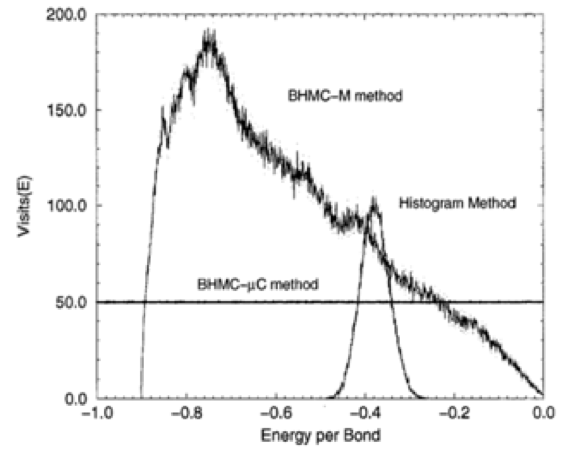
\includegraphics[height=170pt]{pics/en_bond}
 % \captionof{figure}{}
  \label{fig:en_bond}
\end{minipage}\hfill
\begin{minipage}{.49\textwidth}
  \centering
  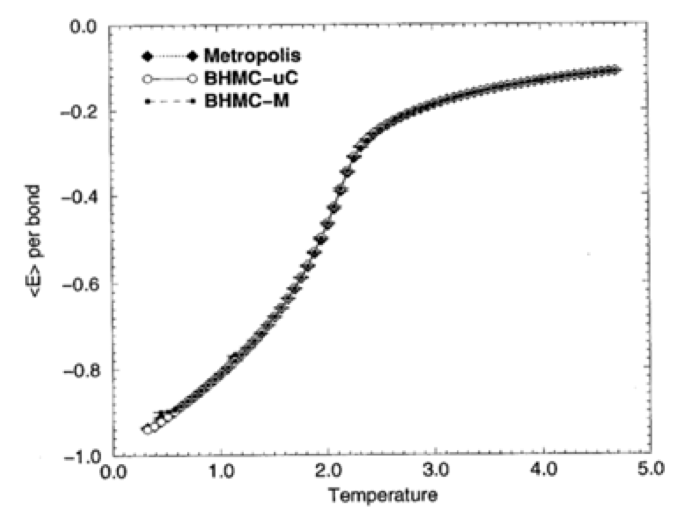
\includegraphics[height=170pt]{pics/e_xy}
  %\captionof{figure}{Number of visits done in the phase space against the energy.}
  \label{fig:e_xy}
\end{minipage}
\end{minipage}
\vspace{0.1cm}



\vspace{0.1cm}
\noindent
\noindent\begin{minipage}{\textwidth}
\begin{minipage}{.99\textwidth}
  \centering
  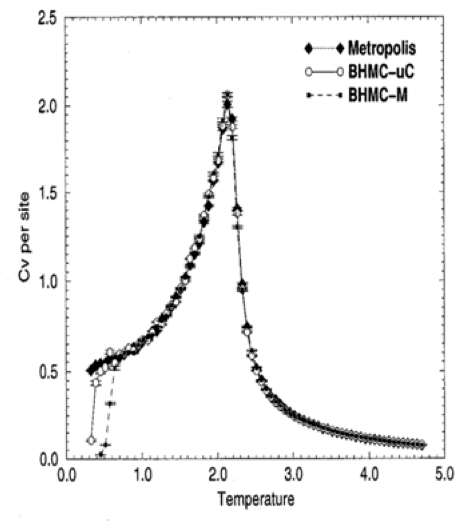
\includegraphics[height=260pt]{pics/cv_xy}
 % \captionof{figure}{}
  \label{fig:cv_xy}
\end{minipage}
\center
Figures: Broad Histogram method for the 3D XY model.
\end{minipage}



\subsection{Implementation of Cluster Algorithms}

\subsubsection*{Swendsen-Wang algorithm:}

The Swendsen-Wang algorithm is a refined Monte Carlo technique. For a certain configuration, we look through the bonds connecting the spins. Whenever two bonded sites  are in the same state, the two sites belong to the same cluster with probability $p\equiv 1-e^{-\beta J}$. Once the clusters are determined, they can be flipped using any of the dynamics mentioned above. The basic procedure is as follows:
\begin{itemize}
\item Occupy the bonds with probability $p\equiv 1-e^{-\beta J}$ if sites are in the same state.
\item Identify the clusters with the Hoshen-Kopelman algorithm.
\item Flip the clusters with probability 0.5 for Ising or choose always a new state for $q>2$.
\item Repeat the procedure.
\end{itemize}

\vspace{0.2cm}

\noindent\begin{minipage}{\textwidth}
\begin{minipage}{.98\textwidth}
  \centering
  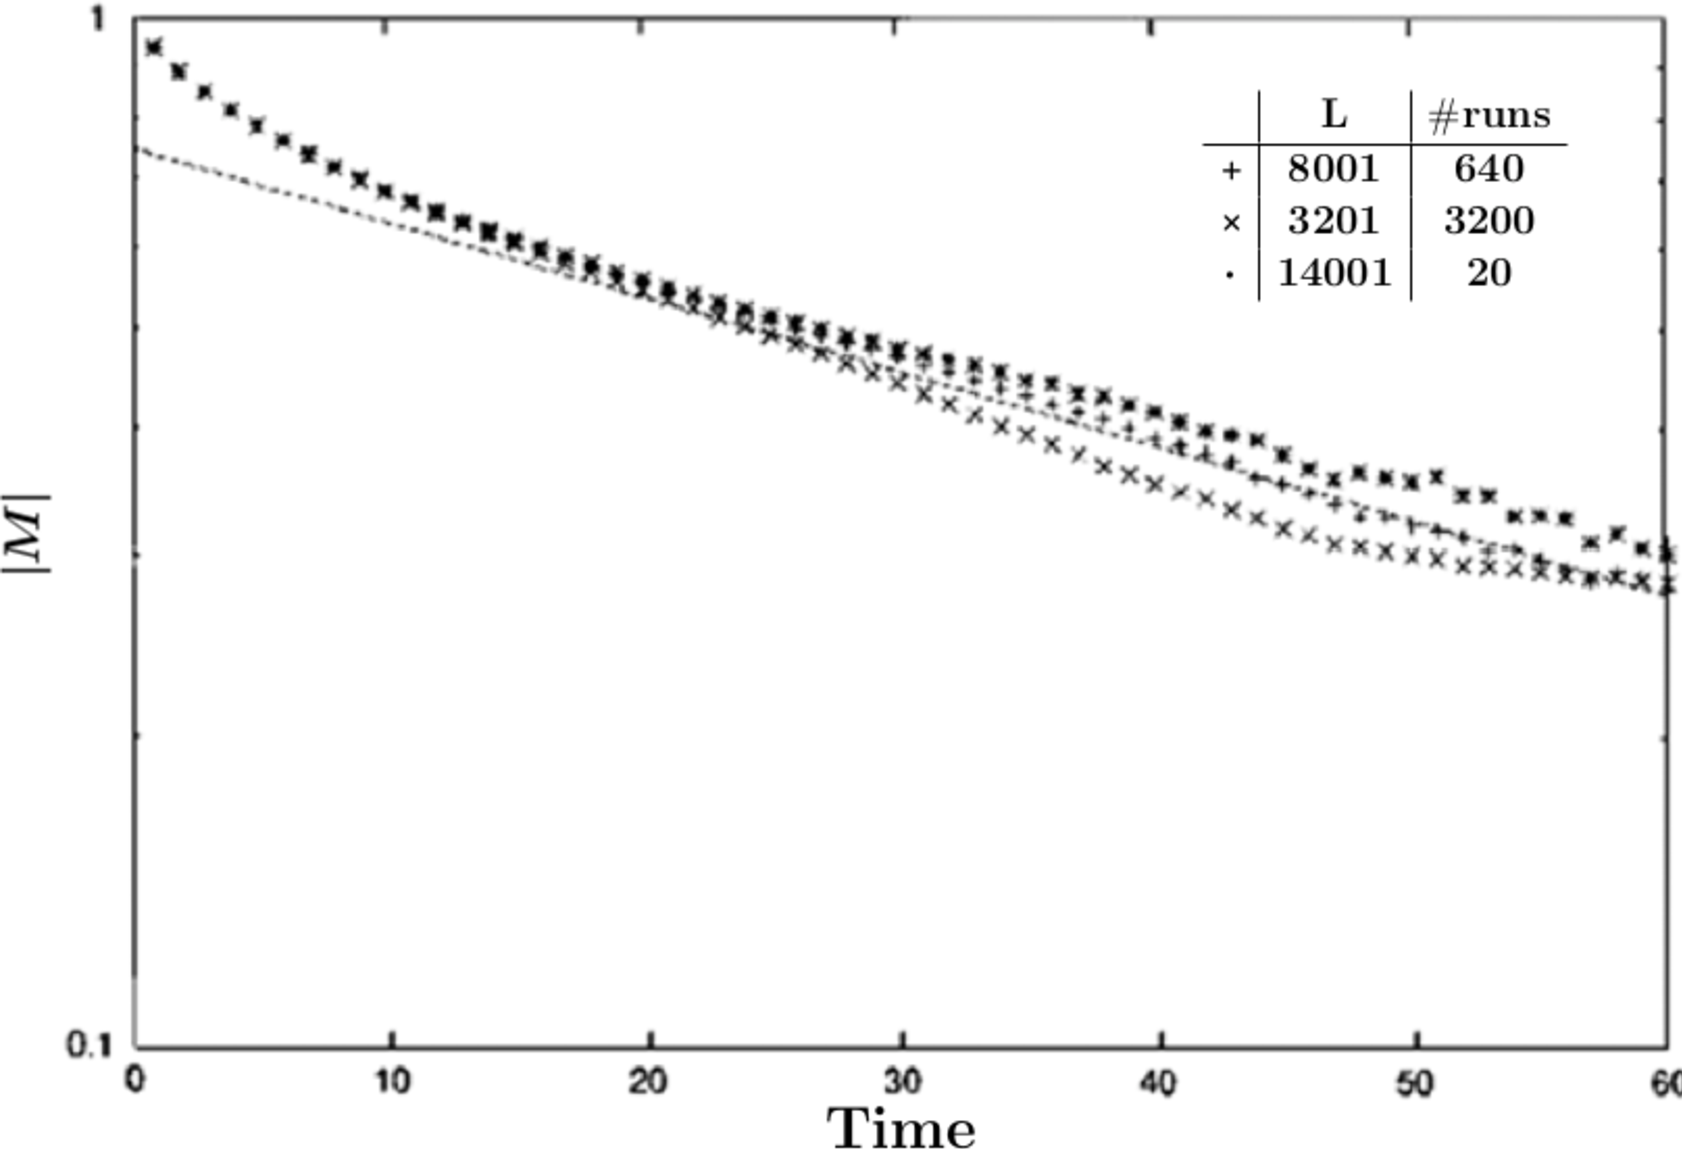
\includegraphics[width = 0.8\textwidth]{pics/critical_slowing_down_swendsen}
  \captionof{figure}{Critical slowing down for the Swendsen-Wang algorithm.}
  \label{fig:critical_slowing_down_swendsen}
\end{minipage}
\end{minipage}

\subsubsection*{Wolff algorithm:}
In this variant only one cluster is flipped per step using the \emph{Leath algorithm}:

\begin{itemize}
\item Choose a site randomly.
\item If neighboring sites are in the same state, add them to the cluster with probability $p\equiv 1-e^{-\beta J}$.
\item Repeat this for any site on the boundaries of the cluster, until all the bonds of the cluster have been checked exactly once.
\item Choose any new state for the cluster.
\item Repeat the procedure.
\end{itemize}



\section{Histogram Methods}

Histogram methods go back to \citet{salzburg}. To reduce the computational cost, one can compute a certain quantity at a given temperature and then extrapolate the result to other temperatures. This is only possible if the temperature dependence is known. In the case of canonical variables the dependence is given by the Boltzmann factor. As a start, the partition function is reformulated as a sum over all possible energies instead of over all possible configurations:
\begin{equation}
Q\kl{T} = \frac{1}{Z_T}\sum_E{Q\kl{E} p_T\kl{E}}\text{\hspace{0.2cm}with } Z_T=\sum_E{p_T\kl{E}}
\label{eq:part_fun_over_energy}
\end{equation}
where $p_T\kl{E} \equiv g\kl{E} e^{-\frac{E}{k_BT}}$ with $g\kl{E}$ being the \emph{density of states} (i.e. the number of states with energy $E$). This takes into account the fact that more configurations can have the same energy. The goal is to compute the quantity $Q$ at another temperature $T^*$:  $Q\kl{T^*} = \frac{1}{Z_T^*}\sum_E{Q\kl{E} p_T^*\kl{E}}$. The density of states contains all the information needed. Using the definition of $g\kl{E}$ yields 
$$p_{T^*}\kl{E}=g\kl{E}e^{-\frac{E}{k_BT^*}} \underbrace{=}_{\text{def. of $g\kl{E}$}}  p_T\kl{E}exp\ekl{-\frac{E}{k_BT^*}+\frac{E}{k_BT}}
$$
and with $f_{T,T^*}\kl{E}\equiv exp\ekl{-\frac{E}{k_BT^*}+\frac{E}{k_BT}} $ one finally obtains
\begin{equation}
Q\kl{T^*} = \frac  { \sum_E {Q\kl{E} p_T\kl{E} f_{T,T^*}\kl{E} }}   {  \sum_E  p_T\kl{E} f_{T,T^*}\kl{E} }.
\label{eq:histo_average}
\end{equation}
We have now obtained an expression for the quantity $Q$ at the temperature $T^*$ without having to measure any distribution at temperature T, since $f_{T,T^*}$ are known scalars. The drawback of this method is that the values of $Q\kl{E}$ are sampled around the maximum of $p_T\kl{E}$, which  converges to a delta distribution for large systems. This means that if $T$ and $T^*$ are not very close, the statistics are very poor, and results will be inaccurate or  even wrong. One possible solution consists of interpolating data from several temperatures (multi-canonical method) but this involves calculations for many temperatures, which is also not efficient for large systems. Another solution to this problem has been presented in \citet{oliveira} and will be also treated in this chapter.
\subsection{Broad Histogram Method}
The aim of the broad histogram method (BHMC) is to directly calculate the density of states. It obtains the function $g(E)$ through a stochastic process. The density of states increases very steeply (exponentially) with energy $E$, since the number of possible configurations increases with higher energy. A plain random walk through phase space would also have the problem that it would explore only the regions with high energies. To explore all the regions equally (with respect to the energy) we can create a Markov chain in which the number of processes that increase the energy by $\Delta E$ (we shall call this number $N_{up}$) and the number of processes that decrease the energy ($N_{down}$) fulfill an equivalent condition to detailed balance to reach a homogeneous steady state:

\begin{equation}
g\kl{E+\Delta E} N_{down}\kl{E+\Delta E} = g\kl{E} N_{up}\kl{E}.
\label{eq:detailed_balance_broad_histo}
\end{equation}
The motion (in phase space) towards higher energies can then be penalized with Metropolis-like dynamics:
\begin{itemize}
\item Choose a new configuration
\item If the new energy is lower, accept the move
\item If the new energy is higher then accept with probability $\frac{N_{down}\kl{E+\Delta E}}{N_{up}\kl{E}}$
\end{itemize}
However, we haven't obtained the function $g\kl{E}$ yet. Therefore we will take the logarithm of Eq. \eqref{eq:detailed_balance_broad_histo} and divide by $\Delta E$


$$
\log \ekl{g\kl{E+\Delta E} } - \log \ekl{g\kl{E} } = - \log \ekl{N_{up}\kl{E} }  - \log \ekl{N_{down}\kl{E+\Delta E} } 
$$
\begin{equation}
\Rightarrow
\pder{\log \ekl{g\kl{E} } }{E} = \frac{1}{\Delta E}\log \ekl{\frac{N_{up}\kl{E}}{N_{down}\kl{E+\Delta E}} }  
\end{equation}
which we can numerically integrate to obtain $g\kl{E}$. Estimates of $N_{up}$ and $N_{down}$ can be obtained by checking if a change of state at each site would increase or decrease the energy. 



\vspace{0.1cm}
\noindent
\begin{minipage}{\textwidth}
\begin{minipage}{.48\textwidth}
  \centering
  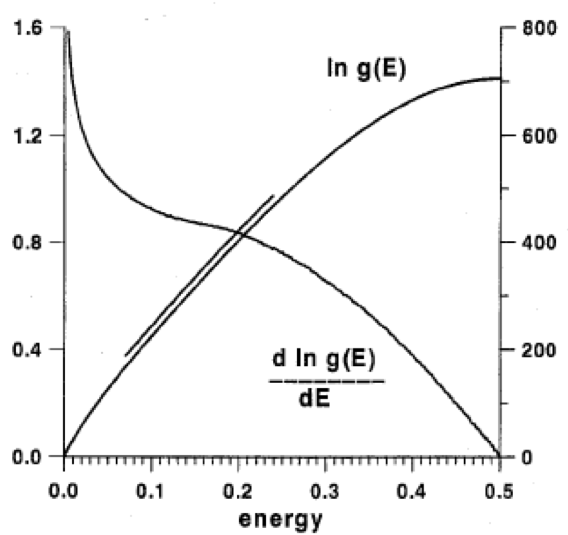
\includegraphics[width = \textwidth]{pics/broad_histo_1}
  \captionof{figure}{Example for the density of states for the Ising model}
  \label{fig:broad_histo_1}
\end{minipage}\hfill
\begin{minipage}{.48\textwidth}
  \centering
  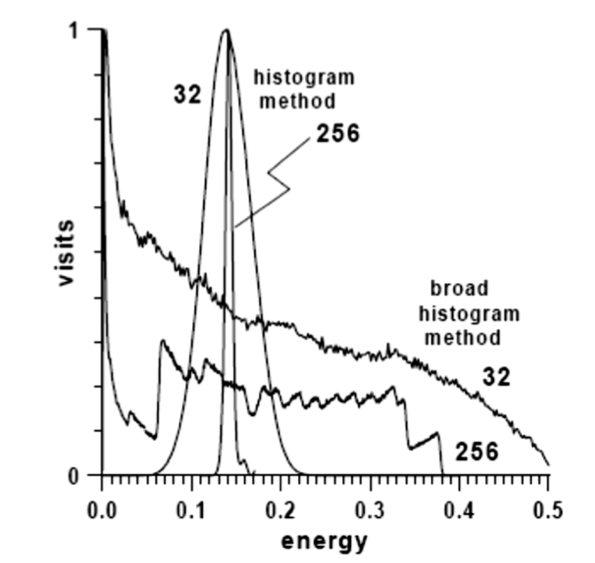
\includegraphics[width = \textwidth]{pics/broad_histo_2}
  \captionof{figure}{Number of visits done in the phase space against the energy.}
  \label{fig:broad_histo_2}
\end{minipage}
\end{minipage}
\vspace{0.1cm}




\vspace{0.1cm}
\noindent
\begin{minipage}{\textwidth}
\begin{minipage}{.48\textwidth}
While moving through phase space one can not only accumulate the values of $N_{up}$ and $N_{down}$, but also keep the values for any quantity $Q\kl{E}$. Finally one can compute
$$
Q\kl{T} = \frac  {\sum_E {Q\kl{E}g\kl{E}e^{-\frac{E}{k_BT}}}  }  {\sum_E {g\kl{E}e^{-\frac{E}{k_BT}}} }
$$
Knowing $g\kl{E}$ one can now calculate quantities at any temperature.
\end{minipage}\hfill
\begin{minipage}{.48\textwidth}
  \centering
  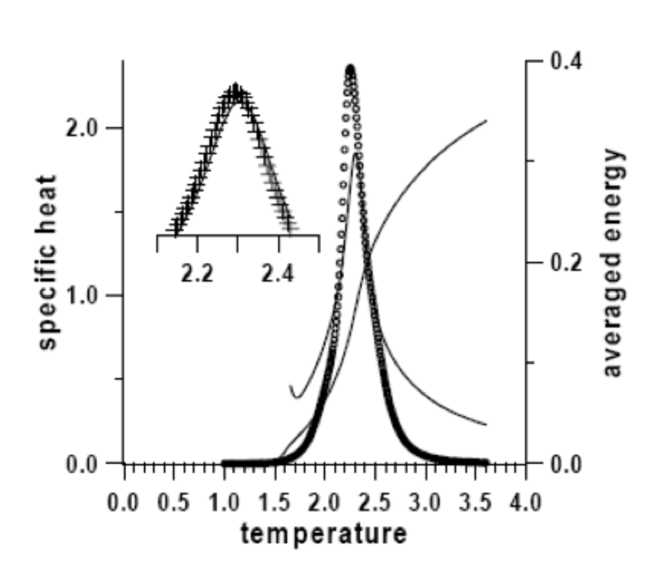
\includegraphics[height=140pt]{pics/broad_histo_3}
 \captionof{figure}{\small The continuous line is the analytic solution of the specific heat for a 32x32 lattice. The crosses represents the result of the BHMC and the circles are the result for the usual histogram.}
  \label{fig:broad_histo_3}
\end{minipage}
\end{minipage}
\vspace{0.1cm}




\subsection{Flat Histogram Method}

This is another method, proposed by Wang, to obtain a flat distribution of visits in energy space. The basic algorithm works as follows:
\begin{itemize}
\item Start with $g\kl{E}=1$ and set $f\equiv E$.
\item Make MC update with $p(E)=1/g(E)$.
\item If the attempt is successful at $E$: $g(E)=f\cdot g(E)$.
\item Obtain a histogram of the energies $H(E)$.
\item If $H(E)$ is flat enough, then $f\equiv \sqrt{f}$.
\item Stop when $f\le 10^{-8}$.
\end{itemize}

Note that choosing the probability as $1/g(E)$ in the second step implies that for higher configuration density at energy $E$, the choosing probability decreases. Therefore the method tends to go towards energies with fewer configurations. At this point the function has to be corrected by updating the value of $g$ and the energy $E$. Once a histogram has been obtained one can increase the precision by decreasing $f$, e.g. by dividing it by two. The ``flatness'' of the histogram can be measured as the ratio of the minimum to the maximum value. For further details, see the \emph{Wang-Landau} algorithm.

\subsection{Umbrella sampling}

This technique was developed and proposed in \citet{torrie}. The aim is to overcome the problem of the lack in ergodicity for certain energy landscapes. As an example, in the Ising model the system could have difficulties in jumping from a positive to a negative magnetization (or vice versa) if the system is very large. The basic idea is to multiply transition probabilities with a function that is large at the free energy barrier and later remove this correction in the averaging step.
\begin{equation}
\tilde{p} \kl{C} = \frac{w\kl{C} e^{-\frac{E\kl{C}}{k_BT}}}{\sum_C{w\kl{C} e^{-\frac{E\kl{C}}{k_BT}}}}
\text{ \hspace{0.1cm} with \hspace{0.1cm} }
\avkl{A} = \frac{\avkl{A/w}_w}{\avkl{1/w}_w}.
\label{eq:torrie}
\end{equation}

\vspace{0.2cm}
\noindent
Summarizing, some of the most common techniques related to the histogram methods are

\begin{itemize}
\item Wang-Landau method 
\item Multiple histogram method
\item Multicanonical MC
\item Flat Histogram method
\item Umbrella sampling
\end{itemize}








\section{Renormalization Group}

In this section, we won't be able to go very deeply into the theory of the subject due to its strong mathematical nature. We will therefore only skim through the main concepts and present some numerical results, for more details see \citet{renorm_leeuwen}.

We will make use of symmetries of the physical system to improve our simulations. Usually, the more information there is available about a system, the better certain quantities can be evaluated. Close to the criticality, changes in the scale of the system can be used to better extrapolate the values to an infinite system. Close to the critical point, one of the most important properties is the invariance under conformal transformations. This also implies the invariance under changes of scale (dilation invariance). Mind that this is only true around $T_c$. To increase mathematical precision one has to define exactly what it means to \emph{change scale}. In the case of geometrical objects, the meaning is somewhat intuitive. A good example is the density in fractals, which does not change under scale transformations (remember the sand-box method in \citet{comp_phys}). However, we wikk also treat systems with different energy and spin configurations as well as different Hamiltonians. One possibility is to look at the free energy density, and its invariance. To renormalize a system means to change its scale by a factor $l$: $\tilde{L}= L/l$.  This can be done either in position, or in momentum (Fourier) space.

\subsection{Real Space Renormalization}




If the system is invariant under a certain transformation, in theory one is able to iterate this transformation infinitely often without changing the quantities in the system\footnote{[...]\emph{We can construct certain transformations on the Hamiltonian of the system for which the critical point is a fixed point. Meaning that observables do not change, no matter how many times we apply these transformations.} \citep{wilson_renorm}}. In other words, the critical point is a \emph{fixed point} for this transformation. In order to put the concept of renormalization in a mathematical framework we will give two concrete examples (renormalization of the free energy and decimation of the 1D Ising model). After that, in sec. \ref{subsec:generalization}, we will generalize the concept and present the implementation of renormalization with MC in sec \ref{subsec:MCRG}. 


\subsubsection*{Renormalization and free energy}
We consider the free energy density of a system, and require it to stays invariant under scale transformations. Since the free energy is an \emph{extensive} quantity\footnote{\emph{Extensive} quantities change with the size of the system, like the volume or the total mass of a gas. \emph{Intensive} quantities are not dependent on the system size, e.g., the energy density or the temperature.}, we have to renormalize the quantity itself to the system size. With $\tilde F$ being the renormalized free energy,
\begin{equation}
\tilde{F}\kl{\tilde{\epsilon},\tilde{H}}=l^{-d} F\kl{\epsilon, H}\text{ with }\epsilon\equiv T-T_c.
\end{equation}
We then make use of the scaling law close to the critical point:
$$
F\kl{\epsilon,H} = l^d F\kl{l^{y_T}\epsilon, l^{y_H}H}
$$
$$
\Rightarrow 
\tilde{F}\kl{\tilde{\epsilon},\tilde{H}} = l^d F\kl{l^{y_T}\epsilon, l^{y_H}H}
$$
\begin{equation}
\Rightarrow 
\tilde{\epsilon} = l^{y_T}\epsilon\text{, }\tilde{H} = l^{y_H}H.
\end{equation}

Since renormalization also affects the correlation length $\xi\propto \abs{T-T_c}^{-\nu}= \abs{\epsilon}^{-\nu}$ we can relate the critical exponent $\nu$ to $y_T$:
$$
\tilde{\epsilon}^{-\nu}\propto \tilde{\xi} = \frac{\xi}{l}
$$
$$
\Rightarrow
\tilde{\epsilon} =\frac{\epsilon}{l^{-\frac{1}{\nu}}} =l^{\frac{1}{\nu}}\epsilon=l^{y_T}\epsilon
$$
$$
\Rightarrow
y_T=\frac{1}{\nu}.
$$
The critical point is a fixed point of the transformation: at $T_c$, $\epsilon=0$, and whatever the value of the scaling factor, $\epsilon$ does not change.

\subsubsection*{Majority rule}


An easy example that can be regarded as renormalization of a spin systems is the \emph{majority rule}. One considers local groups of spins $\sigma_i$, and instead of considering them all separately taking a mean over that local group of spins: $\tilde{\sigma}_{\tilde{i}} =\text{sign}\kl{\sum_{\text{region}}\sigma_i}$ (see Fig. \ref{fig:majority_rule}). Attention must be paid on how the transformation is done. In a one dimensional lattice with up/down spins for example it would be an error to apply this transformation on an even number of spins, since the sign is then not well defined for all the possible situations. The fact that one deals with system of a finite size is also something that has to be taken into account: one can renormalize up to a certain scale, before finite size effects are visible.



\noindent
\begin{minipage}{\textwidth}
  \centering
  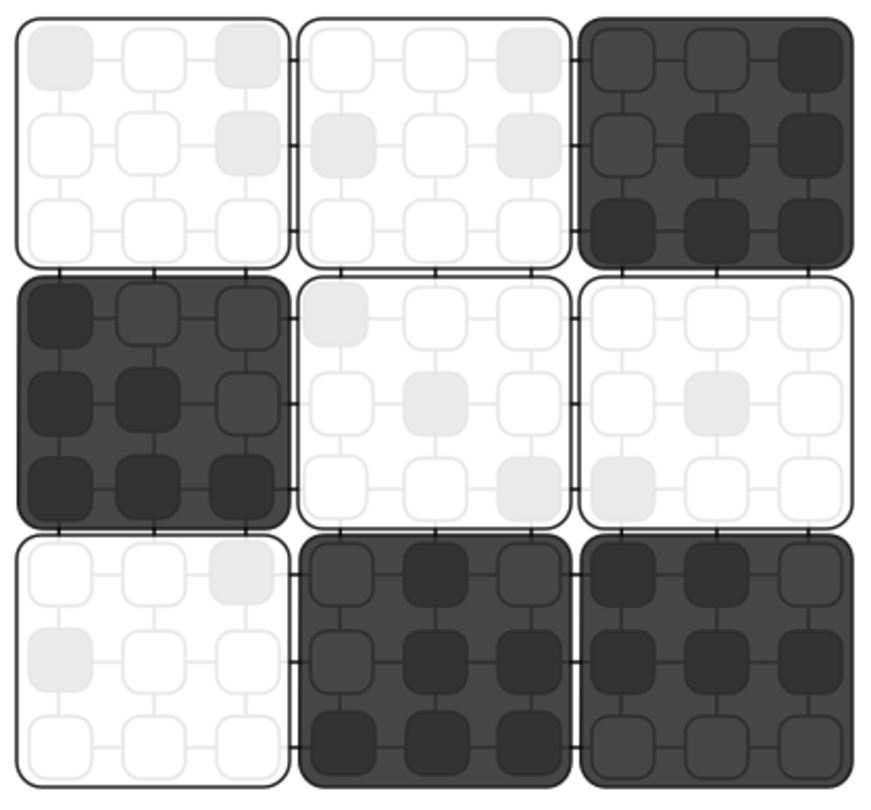
\includegraphics[width=0.5\textwidth]{pics/majority_rule}
  \captionof{figure}{Majority rule for a 2D Ising model. The spins are grouped into larger regions and averaged. If the majority of the spins is in a certain state, that region is considered as a single spin in that state.}
  \label{fig:majority_rule}
\end{minipage}




\subsubsection*{Decimation of 1D Ising Model}


Another possible rule is \emph{decimation} (see Fig. \ref{fig:decimation}). In decimation one just eliminates certain spins, generally in a regular pattern. 
\begin{figure}[h!]
  \centering
  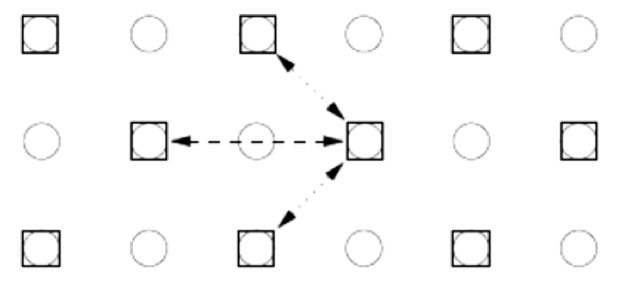
\includegraphics[height=90pt]{pics/decimation}
  \captionof{figure}{Decimation of spins: every second spin in every direction is ignored.}
  \label{fig:decimation}
\end{figure}
\vspace{0.2cm}



As already mentioned, we will consider a one dimensional Ising chain as a practical example. The spins that only interact with their nearest neighbors:

\vspace{0.2cm}

\noindent
\begin{minipage}{\textwidth}
  \centering
  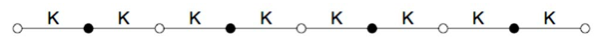
\includegraphics[height=35pt]{pics/1d_decimation}
 % \captionof{figure}{}
  \label{fig:1d_decimation}
\end{minipage}

\vspace{0.2cm}

To see explicitly what happens with the system, we calculate the partition function $Z$. We will split the partition function into two terms: one for the even sites and one for the odd sites. With $K=-\frac{J}{K_BT}$  and using

\begin{align*}
A &= \sum_{s_{2n+1}=\pm 1}{  e^  {K\kl   {  s_{2n}s_{2n+1}  + s_{2n+1} s_{2n+2}     }  } }\\
&=e^  {K\kl   {  s_{2n}+s_{2n+2}    }  }  + e^  {-K\kl   {  s_{2n}+s_{2n+2}    }  } \\
&=\text{cosh}\ekl{K\kl   {  s_{2n}+s_{2n+2}    } }
\end{align*}

we get
\begin{align*}
\mathcal{Z} &= \sum_{s_{2i}=\pm 1}{  \prod_{2i}{   \ekl{ {  
\sum_{s_{2i+1}=\pm 1}{  \prod_{2i+1}{e^  {K\kl   {  s_{2i}s_{2i+1}  + s_{2i+1} s_{2i+2}  }     }  } }  }} } }  \\
&=\sum_{s_{2i}=\pm 1}{  \prod_{2i}{  \mkl{2 \text{cosh}\ekl{K\kl{s_{2i}+s_{2i+2}}}} } }  \\
&=\sum_{s_{2i}=\pm 1}{  \prod_{2i}{  z\kl{K} e^{K' s_{2i}s_{2i+2} } } }  \\
&=\ekl{z\kl{K}}^{\frac{N}{2}}\sum_{s_{2i}=\pm 1}{  \prod_{2i}{   e^{K' s_{2i}s_{2i+2} } } }  
\end{align*}
There are only two possible states, and we can compute $z\kl{K}e^{K's_{2i}s_{2i+2}}= 2\text{cosh}\ekl{K\kl{ s_{2i}+s_{2i+2} }} $ explicitly:

\begin{equation}
z\kl{K}e^{K's_{2i}s_{2i+2}} =\begin{cases}
  2\text{cosh}\ekl{2K}  & \text{for }s_{2i}=s_{2i+2}\\
  2  & \text{for }s_{2i}=-s_{2i+2}
\end{cases}
\label{eq:condition_renorm}
\end{equation}
By dividing and multiplying the two cases we get
$$
e^{2K'} =  \text{cosh}\ekl{2K}  \text{ and } z^2\kl{K} =  4\text{cosh}\ekl{2K} 
$$
$$
\Rightarrow  K' =  \frac{1}{2}\text{ln}\kl{   \text{cosh}\ekl{2K}   }. 
$$
We have now obtained a rule after which the coupling constant $K$ (which contains the temperature and the spin coupling constant $J$) changes under scaling. In summary, we:
\begin{itemize}
\item chose the scaling rule (decimation).
\item imposed the free energy to be constant
\item computed the consequences on the coupling constant $J$
\end{itemize}



 Generally, when renormalizing a system, there are two steps that one has to undertake:
\begin{itemize}
\item Decide which scale to change (e.g., the length of the system, the spins, etc.).
\item Evaluate the consequences for the system (e.g., for the Hamiltonian, the free energy, etc.).
\end{itemize}




\subsection{Generalization}
\label{subsec:generalization}

In the above example it was possible to fulfill the condition of constant free energy with just one coupling constant. Luckily, the transformation rule for the coupling constant $K$ was enough to fulfill all the conditions expressed by eq. \eqref{eq:condition_renorm}. Generally this is not the case, and more coupling constants (e.g., next nearest neighbors) are needed to close the system of equations. We therefore have to construct a renormalized Hamiltonian made up of renormalized coupling constants which generally contain many possible interactions:


\begin{equation}
\tilde{H} = \sum_{\alpha=1}^M{\tilde{K_{\alpha}} \tilde{O}_{\alpha}} 
\text{ with }
\tilde{O}_{\alpha} =  \sum_{i}{\prod_{k\in \epsilon_\alpha}{\tilde{\sigma}_{i+k}}} 
\end{equation}
and with the renormalization rules
$$
\tilde{K}_{\alpha}\kl{K_1,...,K_M},  \text{ with } \alpha \in \mkl{1,...,M}.
$$
Note that using only $M$ interaction terms  instead of an infinite number is a truncation, and in fact a systematic error. The accuracy of this method will depend on the number of iterations that we want to take into account. At $T_c$ we have a fixed point: $\tilde{K}_{\alpha}\kl{K_1^*,...,K_M^*}=K^*_\alpha$. A first ansatz to solve this problem is the linearization of the transformation. We do this calculating the Jacobian $T_{\alpha,\beta} = \pder{\tilde{K}_\alpha}{K_\beta}$:

\begin{equation}
 \tilde{K}_\alpha - K_\alpha^* = \sum_\beta { \left .T_{\alpha, \beta}\right|_{K^*}\kl{K_\beta - K_\beta^*}}
 \label{eq:lin_trafo}
\end{equation}


\vspace{0.1cm}
\noindent
\begin{minipage}{\textwidth}
\begin{minipage}{.48\textwidth}
 We can now construct a flow chart of the coupling constant and obtain values for $\tilde{K}$ for each vector $K=\kl{K_1,...,K_M}$. At $T_c$ (where $K=K^*$), we will have a fix point. Fig. \ref{fig:renorm_flow} shows a flow diagram of a renormalization group transformation. It can already be seen that the flow is stable in some directions (the ones in which the system tends to the fixed point) and unstable in others (the ones that lead the system to go away from the fixed point). 
 \end{minipage}\hfill
\begin{minipage}{.48\textwidth}
  \centering
  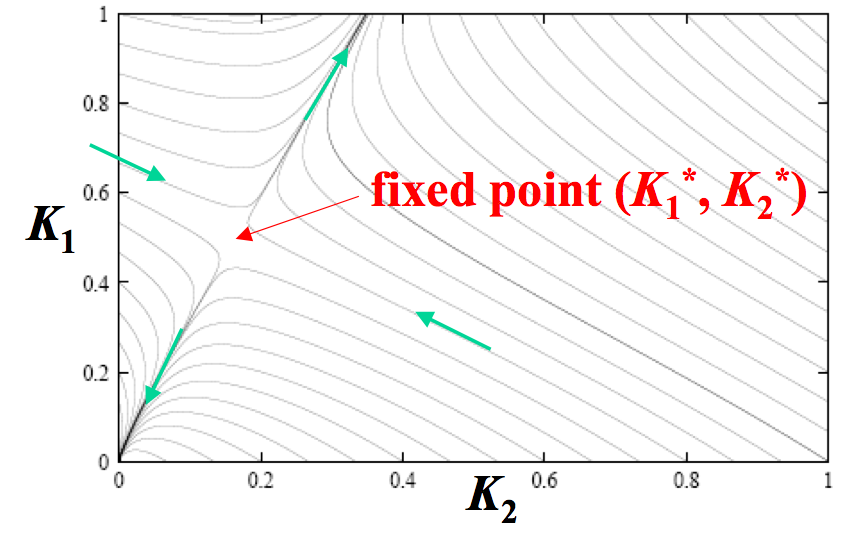
\includegraphics[height=160pt]{pics/renorm_flow}
  \captionof{figure}{Flow diagram of a renormalization transformation.}
  \label{fig:renorm_flow}
\end{minipage}
\end{minipage}

\vspace{0.2cm}


To analyze the behavior of the system close to criticality, we will consider the eigenvalues $\lambda_1,...,\lambda_M$ and the eigenvectors $\phi_1,...,\phi_M$ of the linearized transformation \ref{eq:lin_trafo}. From linear algebra we know that $\tilde{\phi_\alpha}=\lambda_\alpha\phi_\alpha$. Clearly, if $\lambda_\alpha>1$ we have an unstable situation (the distance from $\vec{K}*$ increases at every iteration of the transformation). The biggest eigenvalue will be the dominating one (which is the temperature exponent in the Ising model). We can identify the scaling field $\tilde{\epsilon}=l^{y_T}\epsilon$ with the eigenvector of the transformation, and the scaling factor with eigenvalue $\lambda_T = l^{y_T}$,

$$
\Rightarrow \nu = \frac{1}{y_T}=\frac{\text{ln}\ekl{l}}{\text{ln}\ekl{\lambda_T}}.
$$
This means that we can now calculate critical exponents using the scaling behavior of the system, if the scaling factor $l$ is known. 





\subsection{Monte Carlo Renormalization Group}
\label{subsec:MCRG}

The implementation of real space renormalization with Monte Carlo techniques was first proposed by  \citet{ma_renorm} and then reformulated by \citet{swendsen_renorm}. Since we are dealing with generalized Hamiltonians with a lot of interaction terms, we will calculate the thermal average using the operators $O_\alpha$.

\begin{equation}
\avkl{O_{\alpha}} =
\frac    {\sum_\alpha {O_\alpha e^{\sum_\beta {K_\beta O_\beta}} }  }   {\sum_\alpha {e^{\sum_\beta {K_\beta O_\beta}}}  } =
\pder {F}{K_\alpha}
\label{eq:op_av}
\end{equation}
where $F=\text{ln}\ekl{Z}$ is the free energy. Using the fluctuation-dissipation theorem one can also numerically calculate the response functions:
\begin{align*}
\chi_{\alpha,\beta} &\equiv \pder{\avkl{O_\alpha}}{K_\beta} = \avkl{O_\alpha O_\beta} -\avkl{O_\alpha }\avkl{ O_\beta}\\
\tilde{\chi}_{\alpha,\beta} &\equiv \pder{\avkl{\tilde{O}_\alpha}}{K_\beta} = \avkl{\tilde{O}_\alpha O_\beta} -\avkl{\tilde{O}_\alpha }\avkl{ O_\beta}
\end{align*}
Using the chain rule,  one can calculate with equation \eqref{eq:op_av} that



$$
\tilde{\chi}_{\alpha,\beta} \equiv \pder{\avkl{\tilde{O}_\alpha}}{K_\beta} =
\sum_\gamma {     \pder{\tilde{K}_\gamma}{K_\beta}    \pder{\avkl{\tilde{O}_\alpha^{\kl{n}}}}{K_\gamma}    }  =
\sum_\gamma  {   T_{\gamma, \beta}  \chi_{\alpha,\gamma}^{\kl{n+1}}  }.
$$
Thus we can obtain $T_{\gamma, \beta}$ from the correlation functions by solving a set of M coupled linear equations. We can iterate this method, in order to get systematically better values, if we are at the point $K=K^*$.

\vspace{0.1cm}
\noindent
\begin{minipage}{\textwidth}
\begin{minipage}{.98\textwidth}
  \centering
  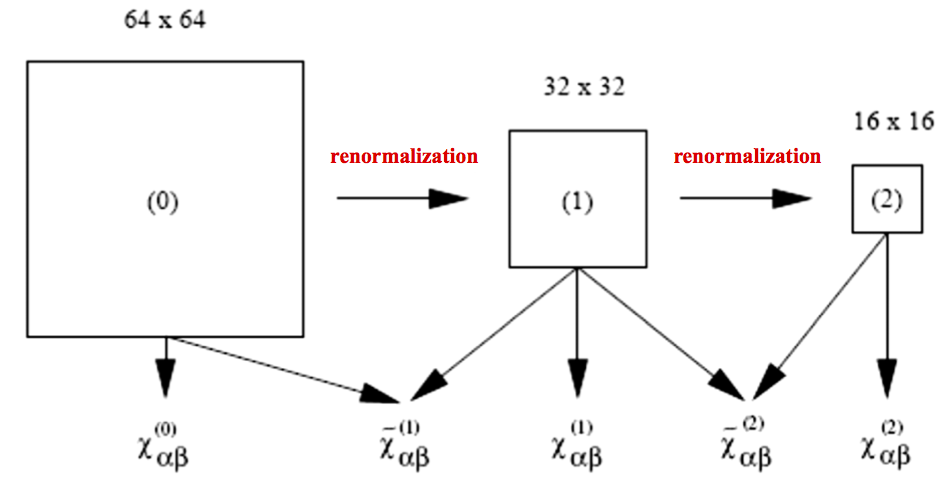
\includegraphics[height=210pt]{pics/mc_renorm}
  \captionof{figure}{Scheme of the MCRG strategy.}
  \label{fig:mc_renorm}
\end{minipage}
\end{minipage}
\vspace{0.1cm}



\vspace{0.1cm}
\noindent
\begin{minipage}{\textwidth}
\begin{minipage}{.98\textwidth}
  \centering
  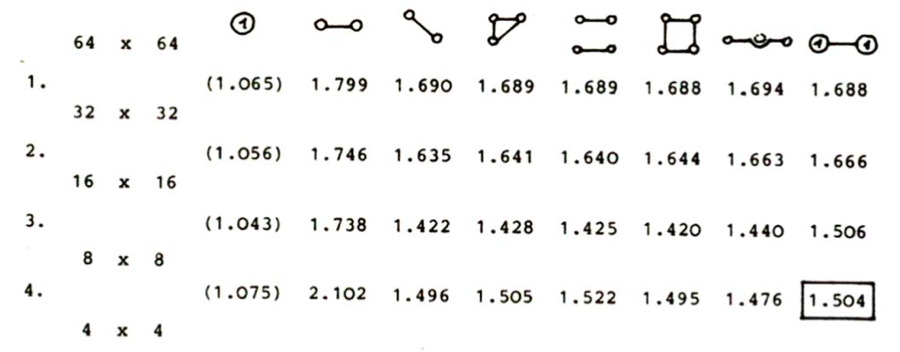
\includegraphics[height=170pt]{pics/nu4_potts}
  \captionof{figure}{$\nu$ for a 4-state Potts model in 2D. Note the convergence.}
  \label{fig:nu4_potts}
\end{minipage}
\end{minipage}
\vspace{0.1cm}



\subsubsection*{Errors in MCRG}

There are many error sources in this technique, that originate from the fact that we are using a combination of several tricks to calculate our results, of which one should be aware of:

\begin{itemize}
\item Statistical errors
\item Truncation of the Hamiltonian to the M$^{th}$ order.
\item Finite number of scaling iterations
\item Finite Size effects
\item No precise knowledge of $K^*$
\end{itemize}


















%------------------------------------------------------------------------------------------------------------------------------------------


\chapter{Parallelization}
\label{chap:parallelization}

In this short Chapter we will briefly discuss the main methods for making computations faster in a very general way. Parallelization can lead to an improvement of the computation time of up to entire orders of magnitude! The easiest way to parallelize is by \emph{farming}: repeating the same calculations on many different computers/processors with different data. This can be very easy to program in situations like Monte Carlo, where one has to repeat the exact same sequence of operations as many times as possible. Of course, this is mostly not regarded as smart parallelization.  Already with some very basic knowledge of computer architecture there is the possibility of drastically improving the efficiency of the programs.  Two ways to parallelize, which imply a little deeper understanding of how a computer works, are presented in the chapter (\textbf{multi-spin coding} and \textbf{vectorization}). The chapter is obviously not exhaustive, and for the interested reader dedicated lectures are recommended.


\section{Multi Spin Coding}
\label{sec:multi_spin}

Multi spin coding is a technique to reduce the computational time of a program. It is very useful whenever dealing with single bit variables or integers limited to a certain value. The idea is based on the fact that on a 64 bit system, not all the bits are used for storing and/or for computations. In the case of the Ising model, we are dealing with spins that can only assume two values $\sigma \in \mkl{\pm 1}$. This means that storing and calculating our site values into 64 bit integers is not only a waste of memory, but also a waste of computation time since most of the bits are not carrying any information. In a cubic lattice, the local field can only assume values $h_i \in\mkl{0, \pm 2, \pm 4, \pm 6} $, for a total of $7$ possible values. 3 bits\footnote{In binary code you can represent up to 8 different numbers with 3 digits} would then be enough to cover all possible local field values of any site $\sigma(i)$, while 61 bits remain unused. If we contemplate an integer variable E, with bit values $\delta \in \mkl{0,1}$,
$$
E_j = (\delta_1,...,\delta_{64})
$$
it is possible to use every three digits for the local field of a site i
\begin{equation}
E_j = (\delta_1,\underbrace{\delta_{2},\delta_{3},\delta_{4}}_{\sigma(i+20)},...,\underbrace{\delta_{62},\delta_{63},\delta_{64}}_{\sigma(1)})
\end{equation} 
And for the values of the spin on the sites we can use another integer N:
\begin{equation}
N_j = (\delta_1,...,\underbrace{0,0,\delta_{3i-2}}_{\sigma(i)},...,\underbrace{0,0,\delta_{1}}_{\sigma(1)})
\end{equation} where the value of $\delta_{3i-2}$ defines the $i^{th}$ spin. This way, only one bit remains unused, instead of 63 (or 31, depending on the computer architecture). The price that one has to pay is that we must be carefulabout how we organize the storage of the variables in the words. This is because neighboring variables should not be stored in the same word.  As mentioned before, besides a purely memory storage question, the main advantage is a much faster calculation. For this we will make use of bitwise logical functions XOR, AND and OR ($\oplus, \wedge$ and $\lor$). First, to extract the information about one site out of an integer, we will define the \emph{mask}: $7 \equiv (0,...,0,1,1,1)$. This can be used to fetch the value out of the last three digits of an integer $N_j$, as defined before.
\begin{equation}
7\wedge N_j = (0,...,0,1,1,1) \wedge_{bitwise} (\delta_1,...,\delta_{62},\delta_{63},\delta_{64}) = (0,...0,\delta_{62},\delta_{63},\delta_{64})
\label{eq:fetch}
\end{equation}
With the circular right shift operator (\emph{ror}) or the circular left shift operator (\emph{lor}) one can act a clockwise (or counter-clockwise) permutation of the bits stored in an integer variable
\begin{equation}
ror\ekl{(\delta_1,\delta_2,\delta_3,\delta_4,\delta_5),2} = (\delta_4,\delta_5,\delta_1,\delta_2,\delta_3)
\label{eq:ror}
\end{equation}


Combining the two operations defined in equations \eqref{eq:fetch} and \eqref{eq:ror} allows us to fetch all the 21 sites or energy values stored in an integer. Similarly for the calculation of the energy, only one cycle is needed to calculate the energy of 21 sites:
\begin{equation}
E_j =N_j \oplus N_{right}  + N_j \oplus N_{left} +,...+,N_j \oplus N_{down}  
\end{equation} 
For an example of implementation in C/C++, see \ref{code:multi_spin}.













\section{Vectorization}

\subsubsection*{Multiple instruction - single data:}

Vectorization means organizing the routines in such a way that many operations can be done simultaneously. Vectorization only works in the innermost loops. As an example

\small
\begin{lstlisting}[frame=single]

i_max = 10000;
for(i=1; i<=i_max; i++){

	A(i) = B(i) * (C(i) + D(i));

}
\end{lstlisting}
\normalsize
In the loop, one has to do several operations: fetch the values of the vectors A,B,C,D, multiply them, adding etc. ... The aim is to parallelize all these operations in a pipe. This is usually already implemented in the compilers, so that the user does not have to care about it. In more complicated routines this may have to be implemented directly. The bad features for vectorization of a routine include

\begin{itemize}
\item Short loops.
\item Conditional branchings like if-statements.
\item Indirect addressing.
\end{itemize}

If the loop is smaller than the ``assembly line'' then there's no need to bother programming in a vectorized way (i.e. if $i_max$ in the upper example would be 4 or 5). Another problem is that the instructions must be repetitive without interruptions or exceptions like if-statements. There are ways to handle some cases in which a distinction is needed, but this is often a problem. An example would be replacing 
\small
\begin{lstlisting}[frame=single]
if(P(i)>z){
	s = -s;
}
\end{lstlisting}
\normalsize
by
 \small
\begin{lstlisting}[frame=single]
s = s*sign(z-P(i));
\end{lstlisting}
\normalsize


In order for vectorization to be maximally exploited, one has to make sure that the inner loop is the largest. One can, for example, transform a n-dimensional system in a one dimensional system using helical boundary conditions and appropriate indexing. Other important elements of an efficient vectorized routine are

\begin{itemize}
\item Make update in inner loop, i.e. no loops inside this loop.
\item Use a vectorized random number generator.
\item Split up loops that cannot be vectorized.
\end{itemize}



\subsubsection*{SIMD vs MIMD:}

There are many types of parallelization, but one can roughly divide them into two groups according to the flexibility of the process and accessibility of your memory access: \emph{Single Instruction - Multiple Data} (SIMD) and \emph{Multiple Instruction - Multiple Data}. In the first case one applies the same set of instructions to all the data. In the second one, different instructions are applied to different data, with the drawback that the routines loose simplicity. There are \emph{shared memory} computers which have the advantage that they are really flexible in the organization of the data structure and \emph{distributed memory} computers which are much easier to build and program. Finally, there is the possibility of combining a great number of processors, each of them with very basic features or a smaller number of more powerful processors (\emph{coarse graining} vs \emph{fine graining}). For each combination there exist different solutions with different programming philosophies. 

\vspace{0.3cm}

$
\centering
\begin{array}{ccc}
\text{SIMD}  & \leftrightarrow  & \text{MIMD}\\
 \hline
 \text{shared memory}  & \leftrightarrow   & \text{distributed memory}\\
 \text{coarse grained}  & \leftrightarrow   & \text{fine grained}\\ 
\end{array}
$

\vspace{0.3cm}





\subsubsection*{MC parallelization:}

Monte Carlo on regular lattices is well suited for parallelization because of a number of reasons:

\begin{itemize}
\item Local processes that do not involve the whole system (nearest neighbors).
\item Domain composition is possible (sub-lattices).
\item Use standard domain decomposition and distribute using in MPI.
\item Use logical mask to extract one sub-lattice.
\item Use periodic shift (CSHIFT) to get neighbors for periodic boundary conditions.
\end{itemize}

There are many options for dividing a system  into domains. Depending on the situations it can be more convenient to increase the domains or reducing the interfaces between the domains in case that the processes need to work independently (e.g., in the case of distributed memory). It is also possible to dynamically change the size of the domains and the position of the interfaces. For an example of parallelization, see Section \ref{code:parallel_pi}.





\noindent
\begin{minipage}{\textwidth}
\begin{minipage}{.98\textwidth}
  \centering
  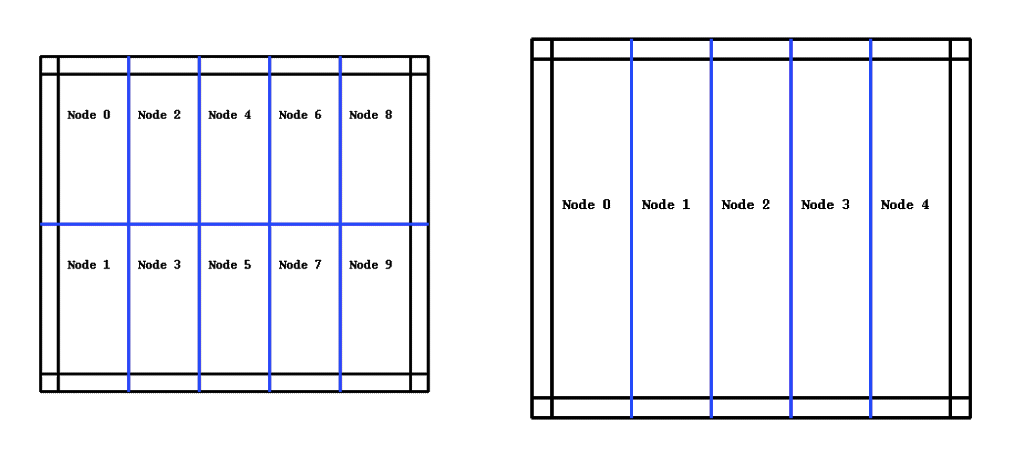
\includegraphics[height=200pt]{pics/node1}
  \captionof{figure}{Domain decomposition of a square lattice.}
  \label{fig:node1}
\end{minipage}%
\hfill
\begin{minipage}{.98\textwidth}
  \centering
  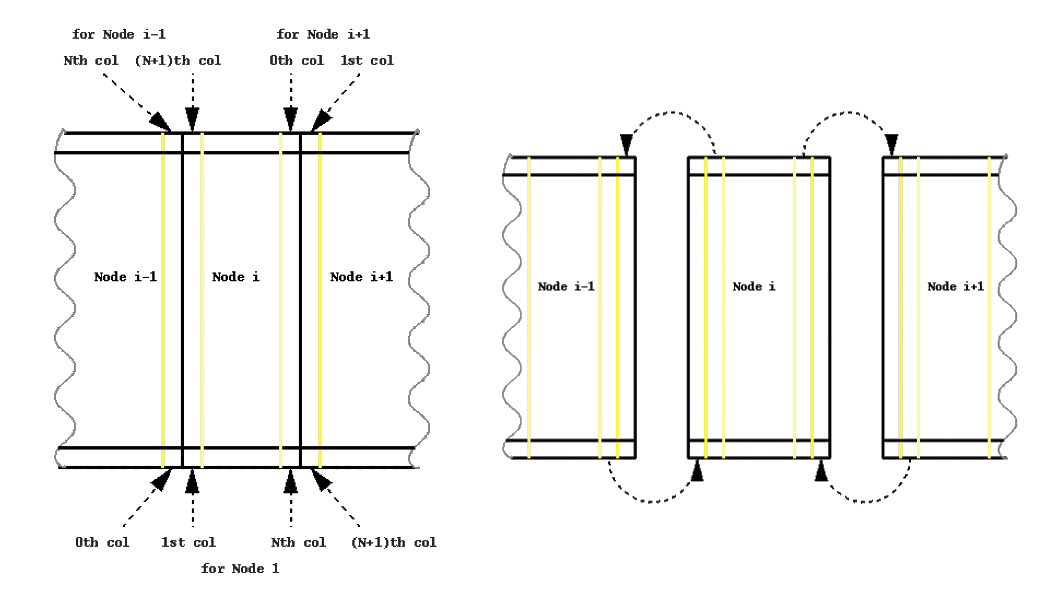
\includegraphics[height=200pt]{pics/node2}
  \captionof{figure}{Different interface setups for domain decomposition of a square lattice}
  \label{fig:node2}
\end{minipage}
\end{minipage}
\vspace{0.1cm}






\subsubsection*{Message Passing Instruction:}

To parallelize a routine one has to use specific programming languages created specifically for parallelizing or embed special libraries in which the parallelization has been implemented in such a way that it can be summoned in standard programming languages such as C++. An interesting example is CUDA (Compute Unified Device Architecture), a parallel computing platform and programming model created by NVIDIA and implemented by the graphics processing units (graphic cards) that they produce. Graphic cards are capable of very fast computation of easy operations, and that can be used in some cases to do scientific computing. \emph{Message Passing Instruction} (MPI) is a standardized and portable message-passing system. This means that instructions can be passed by the user within programs written in languages such as Java or C++. See Section \ref{code:mpi} for basic examples of MPI coding.



\subsubsection*{Amdahl's law:}

The bottleneck of parallelization is the communication between processors. Processors are not isolated units that completely work on their own, and the more one slices the system into domains, the more communication between processors is needed. This is generally not efficient and usually slows down the parallelization.


\vspace{0.1cm}
\noindent
\noindent\begin{minipage}{\textwidth}
\begin{minipage}{.98\textwidth}
  \centering
  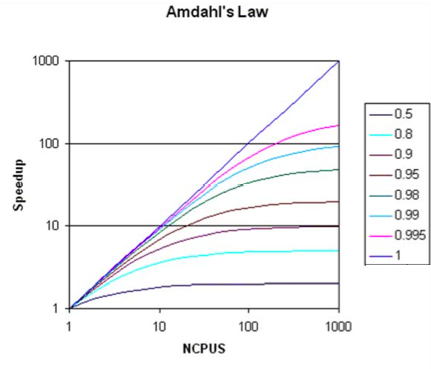
\includegraphics[height=250pt]{pics/amdahl}
  \captionof{figure}{Efficiency of Parallelization. On the right the fraction of parallelized time to total time.}
  \label{fig:amdahl}
\end{minipage}
\end{minipage}
\vspace{0.1cm}












%------------------------------------------------------------------------------------------------------------------------------------------
\chapter{Molecular Dynamics}

\small
After having introduced the problem set, we start with some straightforward methods for solving Newton's equations (\textbf{Verlet} and \textbf{Leap-frog}). The onfollowing parts (\textbf{Lagrange multipliers} and \textbf{long range potentials methods}) make use of more refined mathematical tools to simulate composed or long range interacting particles. A completely different approach to the many-body system is given by \textbf{event driven programming}. This section will conclude the chapter introducing some basic concepts regarding \textbf{inelasticity}. These mentioned methods are of course not the only ones for simulating complex and dynamic systems, but the most intuitive and direct approaches to the problem. This is why \textbf{contact dynamics} and, for the situations in which the complete knowledge of the motion of single particles is not relevant, statistical methods for the simulations of macroscopical quantities are introduced in separate chapters. For further readings,  \citet{sim_liq} is recommended. It contains most of the topics treated in this chapter in a more detailed fashion and gives further references. 

\normalsize
\section{Introduction}

In this chapter we will discuss methods to simulate the motion in many-body systems. We will start describing classical systems (with Newton's equations of motion) and finish with an introduction to ab-initio simulations. Although the mathematical tools are much older\footnote{Numerical methods are almost as old as mathematics itself. Simple calculations such as linear interpolation and square roots approximation were developed a few thousands of years ago (e.g., the Babylonian clay tablet). More refined methods in differential analysis started to become of great interest with the rise of physical science in the $17^{th}$ century. E.g., \emph{Newton's method} or the \emph{Euler Method} that was described by Euler in 1768 and has been certainly known for long time. Even \emph{Runge-Kutta} methods, that are still used today for very precise calculations (for example in celestial mechanics) were developed around 1900.}, the first molecular dynamics (MD) computer simulations were performed in the 1950s. Even if the mathematics is relatively simple and straightforward, it was not possible to do the calculations without computers. This is why, as for Monte Carlo methods, this field started developing in those particular years. Many of the techniques contained in this chapter form the basis of modern commercial softwares. Nowadays, engineering and industry mostly rely on computer simulations for any design and implementation. MD is used in a variety of fields, some examples are:


\begin{itemize}
\item Simulation of atoms and molecules
\item Gravitational interactions
\item Flows dynamics
\item Biopolymers
\item Granular materials
\item Dislocations, voids, quasi-particles
\item Electrons (Car-Parrinello)
\item Explosions
\end{itemize}

\vspace{0.5cm}
\noindent
One of the pioneers of this field is Bernie Alder \citep{alder_first}. He was one of the first to explicitly solve the classical equations of motion using conservation of energy, momentum and invariance under translation and rotation. Using generalized coordinates and momenta of particles in a system where each particle has $\alpha$ degrees of freedom:
$$
\vec{q}_i = \kl{q^1_i,...,q^\alpha_i} 
\hspace{0.2cm} \text{and} \hspace{0.2cm}
\vec{p}_i = \kl{p^1_i,...,p^\alpha_i},
$$
the totality of the system can be described by

$$
Q = \kl{\vec{q}_1,...,\vec{q}_N} 
\hspace{0.2cm} \text{and} \hspace{0.2cm}
P= \kl{\vec{p}_1,...,\vec{p}_N} 
$$
using the Hamiltonian $\mathcal{H}\kl{P,Q} = K\kl{P} + V\kl{Q}$ with $K\kl{P}= \sum_i{  \sum_{k}{  \frac{\kl{p^k_i}^2}{2 m_i}  }  }$ being the kinetic energy and $V$ the potential energy. The evolution of the system is governed by the potential, since it represents all the information about the physical reality that we are simulating (e.g., attractive or repulsive electromagnetic potential). We can expand the potential energy 

$$
V\kl{Q}  = 
\sum_i{V_1\kl{q_i}} +
\sum_i{   \sum_{j> i} { V_2\kl{q_i,q_j}   }} +
\sum_i{   \sum_{j> i} {    \sum_{k > j} {     V_3\kl{q_i,q_j,q_k}     }  }}   + ...
$$


Typically we don't consider all the interactions between more than two (and in some special case, three) particles and we rather treat the different particle-particle interactions using an effective potential:

$$
v^{\text{eff}}_2\kl{q_i,q_j} =  v^{\text{attr}}\kl{r} + v^{\text{rep}}\kl{r}
\hspace{0.2cm} \text{with} \hspace{0.2cm}
r=\abs{\vec{q}_i - \vec{q}_j}
$$
considering (for now) only potentials that depend on distance, not particle orientation. Analytically, the simplest potential is the hard core potential

$$
v^{rep}\kl{r}=\begin{cases}
  \infty,  & \text{for } r<\sigma\\
  0, & \text{for } r\ge\sigma.
\end{cases}
$$
This potential is not well suited for numerical simulations, since the force is infinite at $r=\sigma$. Therefore the potential has to be smoothed and adapted for use in numerical simulations. Depending on the chosen potential, the dynamics will be different, and the computation can be easier or more cumbersome. For example, for long range potentials (like $\propto \frac{1}{r}$) we will have to take into account that the energy diverges at infinity, and we will have to deal with this problem since this kind of potentials are very important in physics.

\section{Equations of Motion}

\subsubsection*{Repulsive and attractive potentials:}
The first order Taylor approximation of a symmetric  attractive or repulsive potential is given by an elastic potential. For two particles with radii $R_1$ and $R_2$, the potential is given by

$$
v^{rep}\kl{r}=\begin{cases}
  \frac{k}{2}\kl{R-r}^2,  & \text{for } r<R\\
  0, & \text{for } r>R
\end{cases}
\hspace{0.4cm} \text{with} \hspace{0.2cm}
R= R_1 + R_2,
$$
where $k$ is the elastic spring constant.

\vspace{0.1cm}

\begin{figure}[h!]
  \centering
  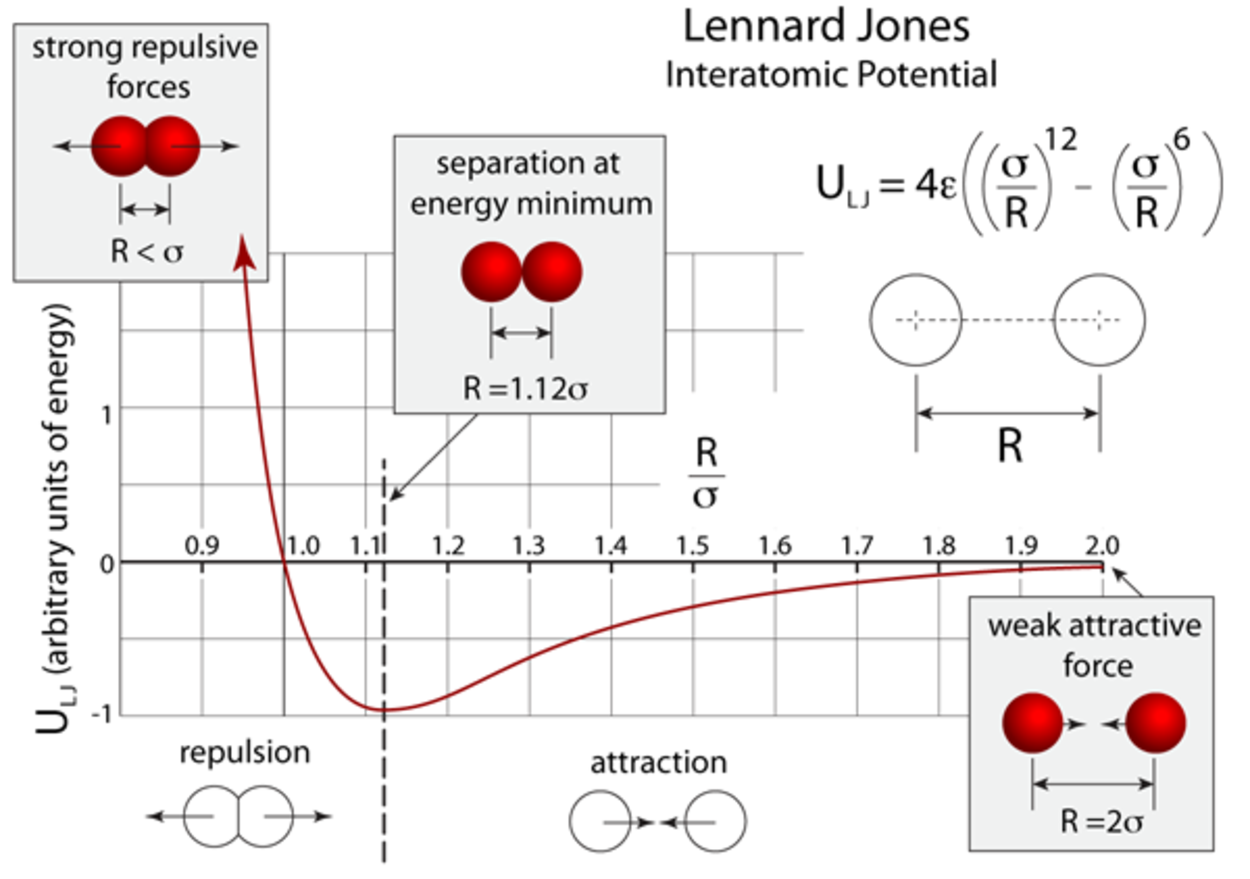
\includegraphics[width=0.8\textwidth]{pics/Lennard_Jones}
  \captionof{figure}{Lennard Jones potential \citep{atoms_in_motion}}
  \label{fig:lennard jones}
\end{figure}

Another very important form of potential typically used to describe the interaction between molecules is the \emph{Lennard Jones} potential (see fig.\ref{fig:lennard jones}). Here $\epsilon$ denotes the attractive energy and $\sigma$ is the interaction range in some arbitrary units. It is a mathematically simple model that approximates the spherical symmetric interaction between a pair of neutral atoms or molecules quite well.


\subsubsection*{Equation of motion:}
Once the interaction potential has been defined we can easily derive the equations of motion using the Hamilton equations:

$$
\dot{\vec{q}}_i^{\,k} =  \pder{\mathcal{H}}{\vec{p}_i^{\,k}},
\hspace{0.2cm}
\dot{ \vec{p}}_i^{\,k} = - \pder{\mathcal{H}}{\vec{q}_i^{\,k}},
\hspace{0.2cm} \text{with} \hspace{0.2cm}
k\in\mkl{1,...,\alpha}
\hspace{0.2cm} \text{and} \hspace{0.2cm}
i\in\mkl{1,...,N}.
$$
In the standard representation ($\vec{q}=\vec{x}$ and $\vec{p}=\vec{v}=\frac{\vec{p}}{m}$) we obtain 

\begin{equation}
\dot{\vec{p}}_i = - \nabla V\kl{Q} =f_i
\hspace{0.2cm} \text{and} \hspace{0.2cm}
m_i \ddot{\vec{x}}_i = f_i = \sum_j {f_{i,j}},
\label{newt_MD_eq}
\end{equation}

where ${f_{i,j}}$ is the force exerted by particle $j$ on particle $i$.

Those are the equations of motion to solve, which can be done by applying various numerical integration techniques (some of them already know from \citet{comp_phys}). When computing the motion of the particles, we should also estimate the precision needed and achieved by our algorithms. As an example of a numerical error, when $\Delta t$ is too large (relatively to the particles' speed), the large integration step causes numerical errors. Intuitively, for too large time steps, particles can pass through other particles' range of interaction without feeling any influence. We therefore need an estimation of the appropriate time step and of the integration error. Such a measure is the \textit{contact time}.

\subsection{Contact time:}
\label{subsec:contact_time}

Since we are only interested in a spherically symmetric interaction that solely depends on distance, we may also reduce our problem to one dimension. Using the equations for energy
$$
E= \frac{1}{2} m\dot{r}^2 + V\kl{r} = \text{constant}
$$ 
and radial velocity
$$
\der{r}{t} = \ekl{\frac{2}{m} \kl{E-V\kl{r}}}^{\frac{1}{2}},
$$
we can derive the contact time

\begin{equation}
t_c \equiv 2\int_0^{\frac{1}{2}t_c} {\text{dt}} = 
2\int_{r_{min}}^{r_{max}} {\der{t}{r}\text{dr}} =
2\int_{r_{min}}^{r_{max}} {    \ekl{\frac{2}{m} \kl{E-V\kl{r}}}^{-\frac{1}{2}}  \text{dr}}.
\label{eq:contact_time}
\end{equation}
$t_c$ can be now used to determine the appropriate time step of the simulation. The time integration of the equations of motion can be done using different schemes:
\begin{itemize}
\item Euler method
\item Runge Kutta method
\item Predictor-Corrector method
\item Verlet method
\item Leap-frog method
\end{itemize}
Here, we will only discuss the last two, which have been developed especially for Newton's equations.

















\section{Verlet Method}

This integration method was developed by Loup Verlet \citep{verlet} to solve the Newtonian equations in a many-body system. The procedure is simple and related to forward Euler integration. Using a Taylor expansion in (real!) time steps $\Delta t$ 

$$
\vec{x}\kl{t+\Delta t} = \vec{x}\kl{t} + \Delta t \vec{v}\kl{t} + \frac{1}{2}\Delta t^2 \dot{\vec{v}}+ ...
$$
$$
\vec{x}\kl{t-\Delta t} = \vec{x}\kl{t} - \Delta t \vec{v}\kl{t} + \frac{1}{2}\Delta t^2 \dot{\vec{v}}+ ...
$$
and adding the two expressions, one obtains
\begin{equation}
\vec{x}\kl{t+ \Delta t} = 2 \vec{x}\kl{t}- \vec{x}\kl{t-\Delta t} +\Delta t^2 \ddot{\vec{x}}\kl{t}.
\label{eq:verlet}
\end{equation}
Using Newton's equation, we can evaluate $\ddot{\vec{x}}\kl{t}$ as
$$
\ddot{\vec{x}}_i\kl{t} = \frac{1}{m_i} \sum_j{f_{i,j}\kl{t}}
\hspace{0.2cm} \text{with} \hspace{0.2cm} 
f_{i,j}\kl{t} = - \nabla V\kl{r_{i,j} \kl{t}},
$$
which we can insert in Eq. \eqref{eq:verlet}. Using $\Delta t \lesssim \frac{t_c}{10}$ (see Sec. \ref{subsec:contact_time}), we obtain the new position of the particle. 

Some general remarks about the Verlet method:
\begin{itemize}
\item Two time steps need to be stored ($t$ and $t-\Delta t$).
\item Velocities can be computed with $\frac{\vec{x\kl{t+\Delta t}} -\vec{x\kl{t-\Delta t}}}{2\Delta t}$.
\item The error of a single iteration is of order $\propto \Delta t^4$, i.e. it is globally a third order algorithm.
\item The numbers which are added are very different in magnitude ($\propto \Delta t^0$ and $\propto\Delta t^2$).
\item Improvable by systematical inclusion of higher orders (very inefficient).
\item The method is time reversible, which allows to estimate the error accumulation by reversing the process and comparing it to the initial conditions.
\end{itemize}



\section{Leap-frog Method}


In this case we will consider velocities at intermediate steps, and proceed similarly as in the forward Euler integration. 

$$
\vec{v}\kl{t+\frac{1}{2}\Delta t} =\vec{v}\kl{t-\frac{1}{2}\Delta t}  + \Delta t \cdot \ddot{\vec{x}}\kl{t}
$$
\begin{equation}
\vec{x}\kl{t+\Delta t} =\vec{x}\kl{t}  + \Delta t \cdot  \vec{v}\kl{t+\frac{1}{2}\Delta t}
\label{eq:leap}
\end{equation}
The leap-frog method has the same order of accuracy as the Verlet method, however both methods differ in the order in which the variables are integrated (see Fig \ref{fig:leap_verlet}).

The analogies and differences between the Leap-frog method

$$
\dot{\vec{v}}\kl{t+\Delta t} =\frac{f \kl{\vec{x}\kl{t}} }{m}
$$
$$
\vec{v}\kl{t+\Delta t} = \vec{v}\kl{t} + \Delta t  \cdot  \dot{\vec{v}}\kl{t+\Delta t}
$$
$$
\vec{x}\kl{t+\Delta t} = \vec{x}\kl{t} + \Delta t  \cdot \vec{v}\kl{t+\Delta t}
$$
and the more classical forward Euler integration
$$
\dot{\vec{v}}\kl{t+\Delta t} =\frac{f \kl{\vec{x}\kl{t}} }{m}
$$
$$
\vec{x}\kl{t+\Delta t} = \vec{x}\kl{t} + \Delta t  \cdot \vec{v}\kl{t}
$$
$$
\vec{v}\kl{t+\Delta t} = \vec{v}\kl{t} + \Delta t  \cdot \dot{\vec{v}}\kl{t+\Delta t}
$$
are clear: both rely on explicit forward integration. The update of the variables is then done in a different order. In the Leap-frog method the position is not updated using the previous velocity, as it is done in the usual Euler method.



\vspace{0.1cm}
\noindent
\begin{minipage}{\textwidth}
\begin{minipage}{.98\textwidth}
  \centering
  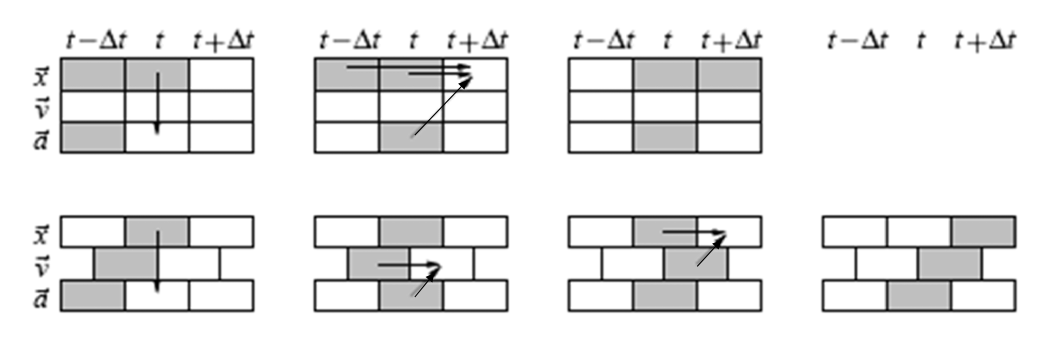
\includegraphics[width=0.95\textwidth]{pics/leap_verlet}
  \captionof{figure}{Comparison of Verlet (upper row) and Leap-frog (lower row) method.}
  \label{fig:leap_verlet}
\end{minipage}
\end{minipage}
\vspace{0.1cm}

Verlet and Leap-frog both use micro-canonical calculations in which energy is conserved. Therefore, for sufficiently small $\Delta t$, energy is usually conserved on average during a simulation. The fluctuations are due to round-off errors. Large fluctuations in energy are usually a hint for either the time step being too large or a bug in the code. The fluctuations of the energy can also be used to estimate the accuracy of the method. 

\vspace{0.1cm}
\noindent
\begin{minipage}{\textwidth}
\begin{minipage}{.98\textwidth}
  \centering
  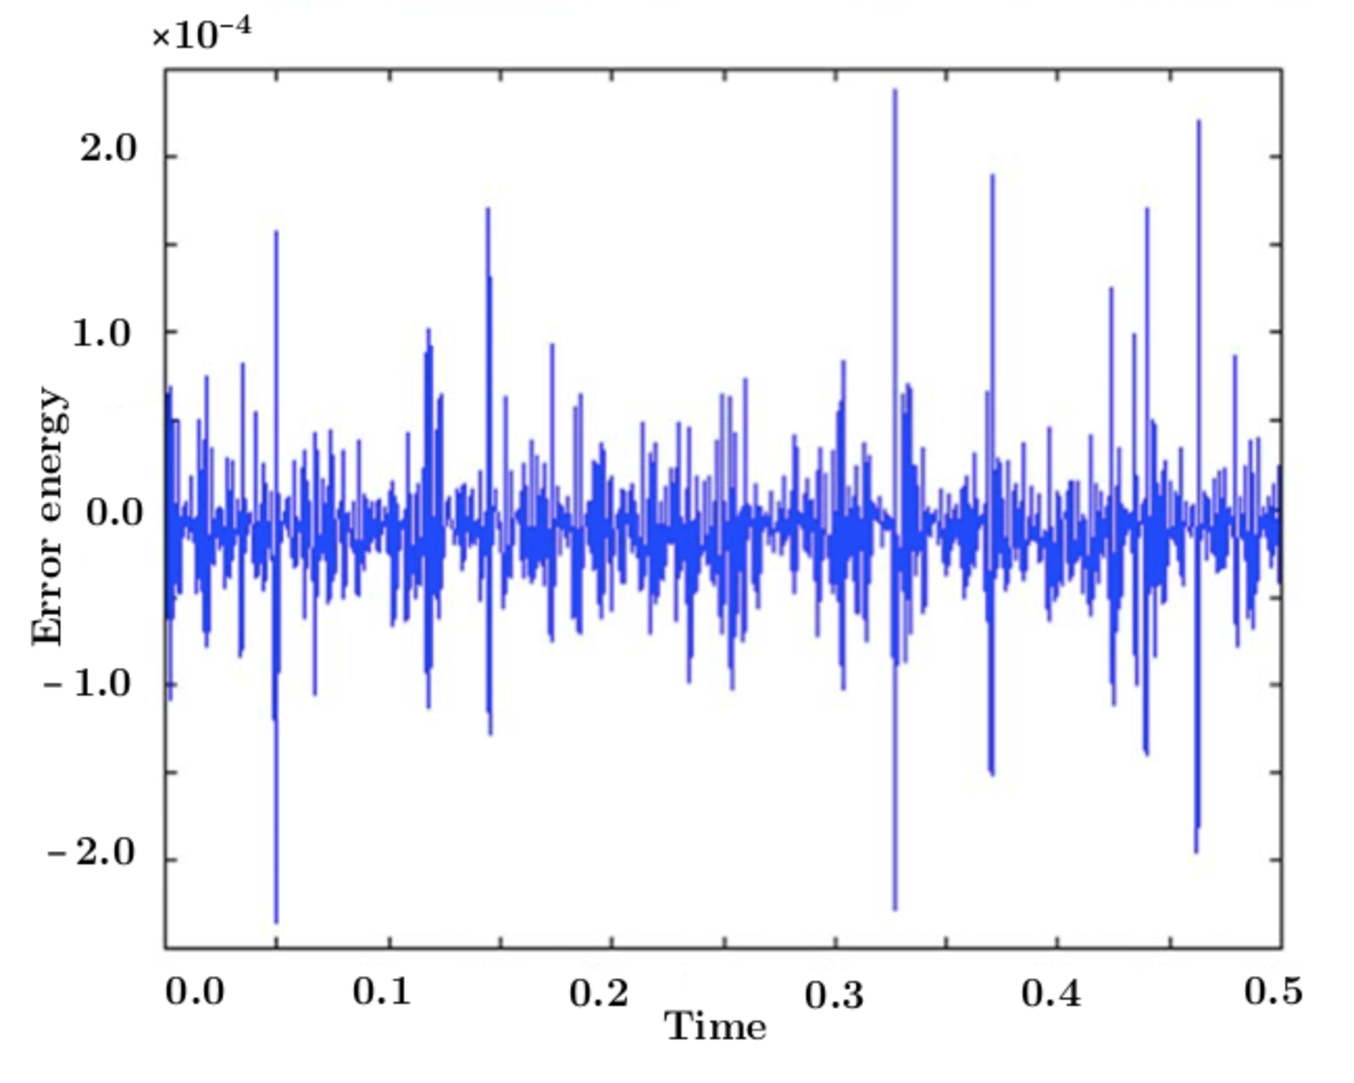
\includegraphics[height=250pt]{pics/energy_leap}
  \captionof{figure}{Energy in the Leap-frog method}
  \label{fig:energy_leap}
\end{minipage}
\end{minipage}
\vspace{0.1cm}

Since these methods are (mathematically speaking) completely time reversible, one can look at the change in the initial configuration after having simulated forward and then backward in time. The difference between the two configurations can be taken as a measure for the error of the method. 

Another approach consists in taking two initial configurations that  differ only slightly in the velocity or the position of a particle, and to observe the difference in time evolution of the two systems. Initially, both systems should behave similarly, but for larger simulation times, the systems will diverge (see Fig \ref{fig:divergence_leap}). The slope of $\log{\Delta E}$ (where $\Delta E$ is the energy difference between both systems) is an indicator of the precision of the method. The slope is called the \emph{Lyapunov exponent}, and it describes the divergence of the simulated trajectory from the true one. More generally, the Lyapunov exponents are related to chaos phenomena which we will not further discuss here. Symplectic integrators by contrast, have the remarkable property to estimate the true trajectory the better the larger the simulation time is. Moreover they preserve the total energy exactly \citep{yoshida}. This allows to simulate Hamiltonian systems such as the three-body problem very efficiently \citep{nagler}.

\begin{figure}[h!]
  \centering
  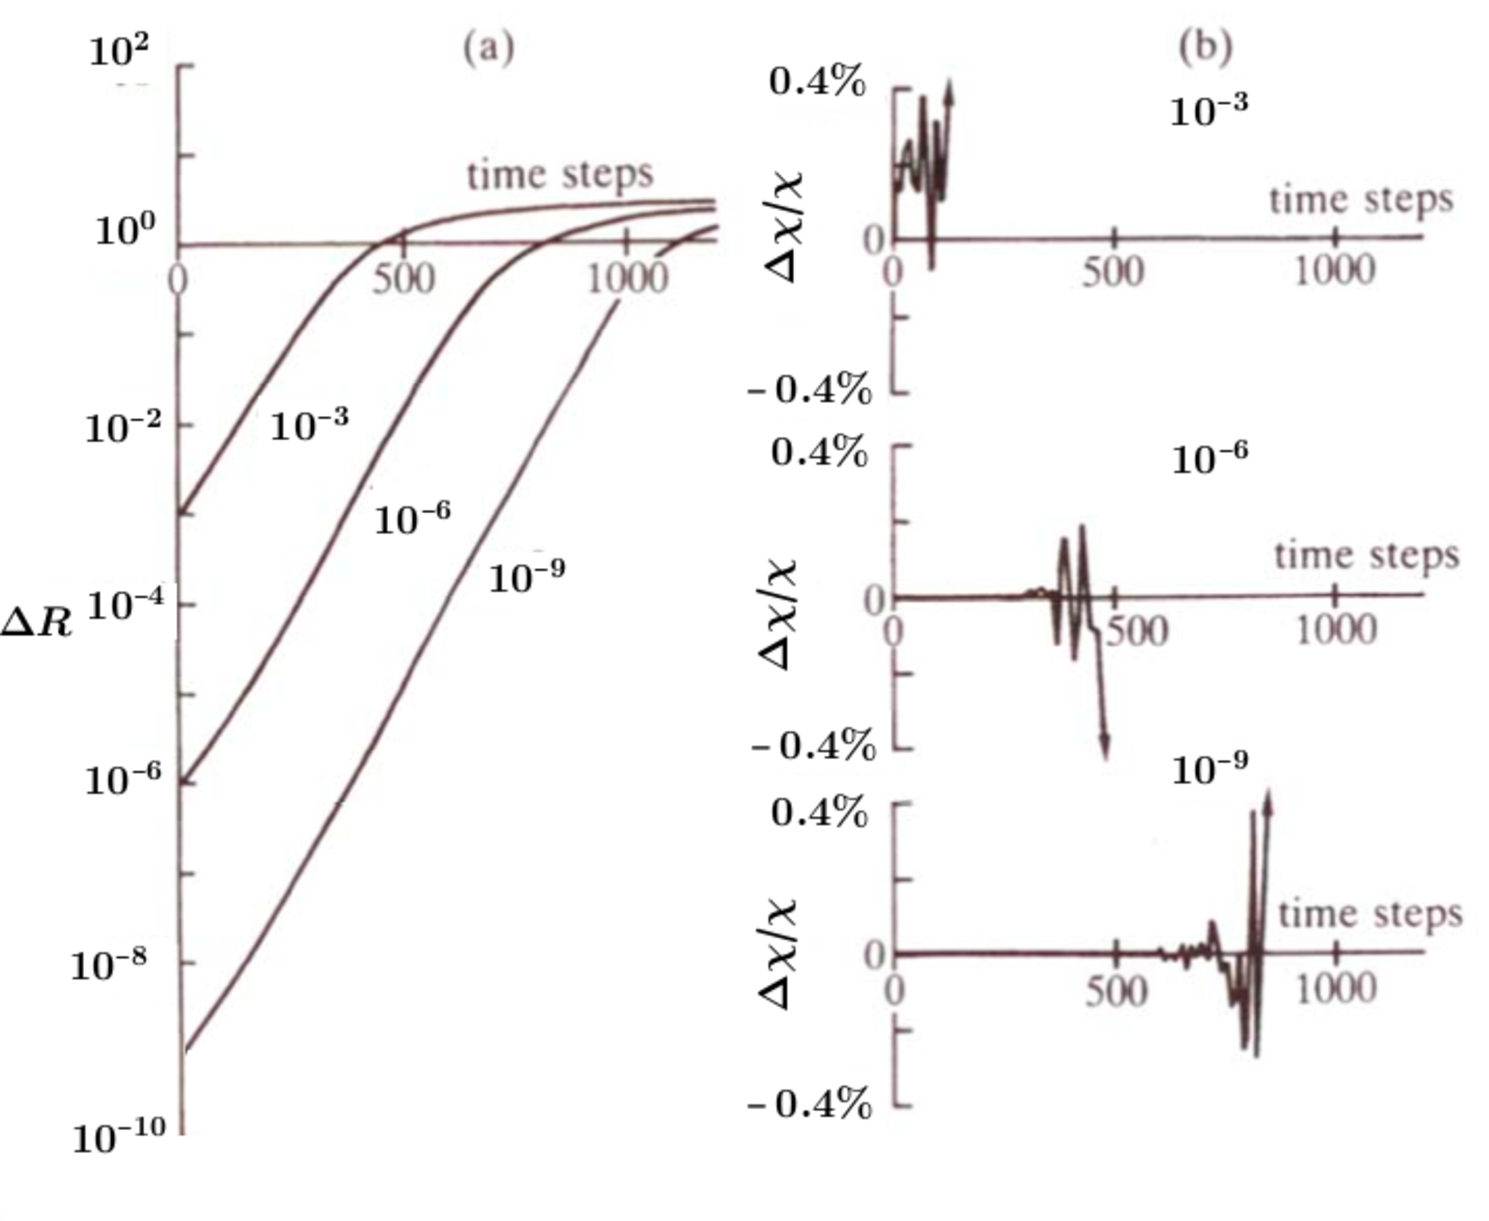
\includegraphics[width=0.6\textwidth]{pics/divergence_leap}
  \captionof{figure}{Comparison of the time development in systems with similar initial configurations. In each system one particle has been placed with an initial position shifted by $\Delta r$. The time evolution of the divergence of the trajectories has been depicted in the right panel, $a$. In the left panel, $b$, the time evolution of the relative energy difference in the the systems.}
  \label{fig:divergence_leap}
\end{figure}

\begin{figure}[h!]
  \centering
  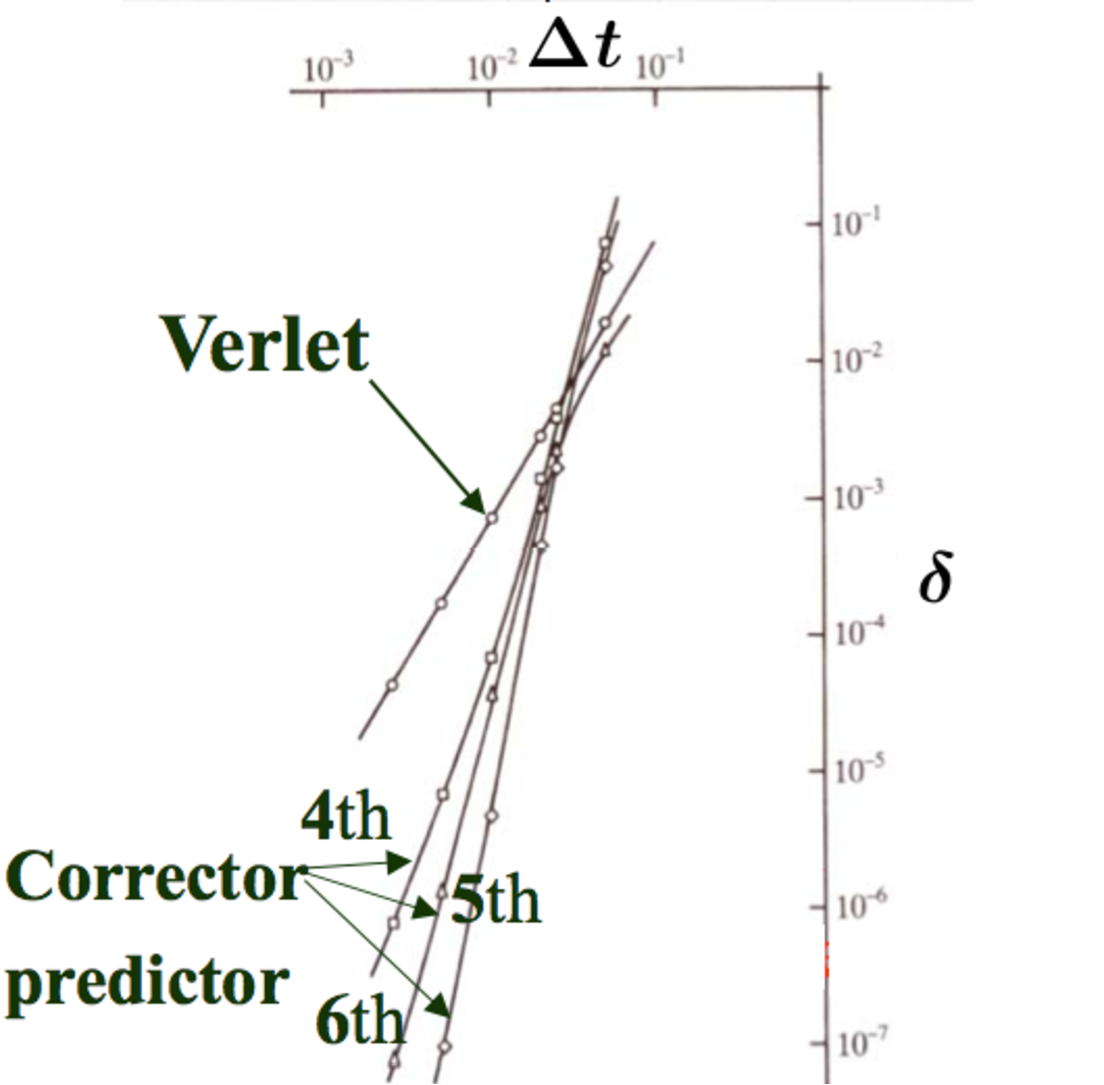
\includegraphics[width=0.5\textwidth]{pics/comp_verlet}
  \captionof{figure}{Comparison of the precision in the Verlet method and the predictor-corrector method of various order.}
  \label{fig:comp_verlet}
\end{figure}



\section{Optimization}

The systems used in MD simulations are usually composed of a large amount of particles. This represents a severe problem, as the computation of all possible pair interactions is very time consuming. e.g. the computation of the force from the potential. If the potential is a function of $\propto r^{y}$ and $y$ is an even number, one can omit the square root to compute the distance between the particles, as the exponent will cancel the square root.

If the potential is not a simple function and its calculation would imply a lot of tedious calculations, one can discretize the potential and sort the values in a look up table. The values can be recalled once the distance of the particle is calculated. The discretization should be chosen in such a way that no important feature is lost. For further precision one can linearly interpolate the bins and correct the values of the look-up table (Newton-Gregory interpolation).

In the case of short range potentials one could think of introducing a cut-off at a distance where the potential is negligible. Mind that this is a problem for $r^{-1}$ potentials since their contribution at very large distances is still not negligible. One can consider the idea of defining a new potential, shifted by a constant, such that it reaches exactly zero at the cut off. This won't affect the forces since any constant disappears when taking the gradient of the potential. Another idea is to interpolate the cut off with a linear (or quadratic) function that reaches zero in a finite distance. Mind that the function is continuous but not smooth at the connection. A careful programmer should be aware of this and address related troublesome situations with caution. Already the first derivative of the potential (i.e. the force) will present a discontinuity, and the second derivative even a divergence where the potential has been interpolated.
 
BLABLA for MADIS, read till here!!

\subsection{Verlet Tables}

\vspace{0.1cm}
\noindent
\begin{minipage}{\textwidth}
\begin{minipage}{.55\textwidth}



In order to reduce the amount of computations one can omit the computation of particle-particle interactions when they are negligible, therefore only particles that are in a certain range have to be considered. One approach to implement such a neighbourhood search is a \emph{Verlet table}, where only the particles in a certain range are stored. As the particles move with time, the table has to be updated regularly, with the updating time being dependent on the implementation of the Verlet table.




\end{minipage}\hfill
\begin{minipage}{.4\textwidth}
  \centering
  \includegraphics[width=\textwidth]{pics/verlet_table}
  \captionof{figure}{In the verlet tables the particles are stored according to their distance from another particle.}
  \label{fig:verlet_table}
\end{minipage}
\end{minipage}
\vspace{0.1cm}


\subsection{Linked Cell Method}

Another method is the \emph{linked cell method} \citep{art}.

\vspace{0.1cm}
\noindent
\begin{minipage}{1.05\textwidth}
\begin{minipage}{.6\textwidth}
In this method, the domain is discretised using a regular grid with grid spacing of, e.g., $\frac{r_c}{2}<M<r_c$, where $r_c$ is the range of the potential (or the cut-off range). We can now identify the cell in which each particle is located. Due to our choice of $M$, only the interaction to particles in a finite number of cells has to be computed, as particles in further cells will not interact with the respective particle. In d dimensions  there are $3^d$ cells of interest (See Fig \ref{fig:linked_cells}). On average we will have to test $N3^d \frac{N}{M^d}$ particles, many of which will not interact with the particle due to their distance. The advantage is that the update of cell populations can be done very efficiently. 
\end{minipage}\hfill
\begin{minipage}{.38\textwidth}
  \centering
  \includegraphics[width=\textwidth]{pics/linked_cells}
  \captionof{figure}{The cells that contribute to the interaction are shaded.}
  \label{fig:linked_cells}
\end{minipage}
\end{minipage}
\vspace{0.1cm}

To look up which particle is in which cell during the computation, one stores in a vector \emph{FIRST} of length $\kl{\frac{L}{M}}^d$ ($L$ is the system size) for each cell $j$ the index of the (arbitrary) first particle in the cell. If the cell is empty, then \emph{FIRST}$\ekl{j}=0$. In a second vector \emph{LIST} of length $N$, the indices of the next particle in the same cell can be stored. If the particle $i$ is the last one in a cell, then \emph{LIST}$\ekl{i}=0$. See \ref{code:linked_cells} for an example on how to program a loop in C to go through all particles in a cell. When a particle changes the cell, \emph{FIRST} and \emph{LIST} can be updated locally, so that no loop over all particles is needed to update the configuration. The algorithm is thus of order $O\kl{N}$.

Additionally, this method is well suited for parallelization. One just has to us the grid to divide the system into domains, which are then each handled by a processor. Cells on the borders can be sent to the neighboring processors using MPI (see Fig. \ref{fig:linked_parallelization}).


\vspace{0.2cm}
\noindent
\begin{minipage}{\textwidth}
\begin{minipage}{\textwidth}
  \centering
  \includegraphics[width=.85\textwidth]{pics/linked_parallelization}
  \captionof{figure}{The System is divided into domains that are treated separately. Each domain is handled by a single processor unit and information can be exchanged using MPI.}
  \label{fig:linked_parallelization}
\end{minipage}
\end{minipage}
\vspace{0.1cm}












\section{Dynamics of Composed Particles}


In nature it is easy to find systems in which the interactions also depends on the size and the shape of the particles (e.g. molecules, crystals, landslides...). To approximate the motion, the interaction and the development of such systems one has to consider the shape and the composition of its composing particles. We will therefore start with the model of rigid bodies, and then relax the condition of rigidity a bit. This implies the following important consideration: it would be an oversight if we would simulate at energies at which the bonds that compose the particles are destroyed. 


\vspace{0.1cm}
\noindent
\begin{minipage}{\textwidth}
\begin{minipage}{.6\textwidth}%
Given the assumption that the bonds are stable in the simulated energy regime, there is a wide range of situations in which these methods are very useful. As an example, at room temperature the  air molecules are not going to break up in their components. The atoms that compose the molecules will also not break up if not in very special situations (ionization in the higher atmosphere or on stars' surfaces, particle accelerators, etc.). As a practical example, consider a water molecule ($H_2O$). In this case, the distance and angles between the atoms are fixed.
 \end{minipage}%
\hfill
\begin{minipage}{.4\textwidth}%
  \centering
  \includegraphics[width=\textwidth]{pics/water}
  %\captionof{figure}{Comparison of the precision in the Verlet method and the predictor-corrector of various order.}
  \label{fig:water}
\end{minipage}
\end{minipage}
\vspace{0.1cm}

There are two main methods applied to such a situation:
\begin{itemize}
\item Lagrange multipliers 
\item Rigid body approximation (good for arbitrary shapes)
\end{itemize}



\subsection{Lagrange multipliers}

\citet{lagrange} were one of the first to propose an extra force term in the equations of motion to impose the constraints given by a speficic shape of the composed particle (e.g. a molecule):

\begin{equation}
m_i\ddot{\vec{x}}_i = \underbrace{f_i}_{\text{external interaction}} + \underbrace{\vec{g}_i}_{\text{internal constraints}}
\end{equation}

We can impose constraining forces that will enforce the geometric arrangement of the molecules, e.g. certain distances $d_{1,2}$ and $d_{2,3}$ between atoms. We can define a potential: such that the constraint forces are proportional to the difference of the actual and the desired distance of the particles:

\begin{align}
\chi_{1,2} &\equiv r^2_{1,2} -d^2_{1,2} \overset{\text{at rest}}{=} 0 \label{eq:chi1}\\
\chi_{2,3} &\equiv r^2_{2,3} -d^2_{2,3} \overset{\text{rest}}{=} 0 \label{eq:chi2}
\end{align}

The equality to zero only holds if the particles have a distance ($r_{ij}$)  equal to the chosen rest position $d_{ij}$. With $r_{ij}\equiv \abs{\vec{r}_{i,j}}$, $\vec{r}_{i,j} \equiv \vec{x}_{i}  -\vec{x}_{j} $ one can obtain
\begin{equation}
\vec{g}_k = \frac{\lambda_{1,2} }{2} \vec{\nabla} _{\vec{x}_k} \chi_{1,2}+
                   \frac{\lambda_{2,3} }{2} \vec{\nabla} _{\vec{x}_k} \chi_{2,3}
\label{eq:g_multip}
\end{equation}
and define the Lagrange multipliers, $\lambda_{1,2}$ and $\lambda_{2,3}$, yet to be determined. We will compute these multipliers by imposing the constraints. The force is then obtained by the gradient of the potential (\eqref{eq:g_multip}):
 \begin{equation}
 \Rightarrow \vec{g}_1 = \lambda_{1,2} \vec{r}_{1,2}, \hspace{0.4cm} 
\vec{g}_2 = \lambda_{2,3} \vec{r}_{2,3} - \lambda_{1,2} \vec{r}_{1,2}, \hspace{0.4cm} 
\vec{g}_3 = - \lambda_{2,3} \vec{r}_{2,3}.
\label{eq:lagrange_forces}
\end{equation}
 This is simply a linear spring with a  yet to be determined spring constant $\lambda$. To obtain the values of $\lambda$, the Verlet algorithm is executed in two steps: first we will compute the positions of the atoms without constraint:
 $$
\tilde{\vec{x}}_i \kl{t+\Delta t} = 2\vec{x}_i  - \vec{x}_i\kl{t-\Delta t} + \Delta t ^2 \frac{f_i}{m_i} 
$$ 
and then we correct the value using the constraints:
$$
\vec{x}_i \kl{t+\Delta t} = \tilde{\vec{x}}_i \kl{t+\Delta t} + \Delta t ^2 \frac{\vec{g}_i}{m_i} 
$$
We can insert \eqref{eq:lagrange_forces} into this last expression to find the updated positions:

\begin{align}
\vec{x}_1 \kl{t+\Delta t} &= \tilde{\vec{x}}_1 \kl{t+\Delta t} + \Delta t ^2 \frac{\lambda_{1,2}}{m_2} \vec{r}_{2,3}\kl{t} \label{eq:blub1}\\
\vec{x}_2 \kl{t+\Delta t} &= \tilde{\vec{x}}_2 \kl{t+\Delta t} + \Delta t ^2 \frac{\lambda_{2,3}}{m_1} \vec{r}_{1,2}\kl{t} -  \Delta t ^2 \frac{\lambda_{1,2}}{m_2} \vec{r}_{1,2}\kl{t} \label{eq:blub2} \\
\vec{x}_3 \kl{t+\Delta t} &= \tilde{\vec{x}}_3 \kl{t+\Delta t} + \Delta t ^2 \frac{\lambda_{2,3}}{m_3} \vec{r}_{2,3}\kl{t}\label{eq:blub3}
\end{align}
With these expressions, we can obtain now $\lambda_{1,2}$ and $\lambda_{2,3}$ by inserting \eqref{eq:blub1}, \eqref{eq:blub2} and \eqref{eq:blub3} into the constraint condition:

$$
\abs{\vec{x}_1 \kl{t+\Delta t} - \vec{x}_2 \kl{t+\Delta t}}^2 = d_{1,2}
$$
$$
\abs{\vec{x}_2 \kl{t+\Delta t} - \vec{x}_3 \kl{t+\Delta t}}^2 = d_{2,3}
$$
$$
\Rightarrow
$$

$$
\abs{      \tilde{ \vec{x}}_1 \kl{t+\Delta t} -\tilde{  \vec{x}}_2 \kl{t+\Delta t} + \Delta t^2 \lambda_{1,2} \kl{\frac{1}{m_1} +\frac{1}{m_2}}\vec{r}_{1,2}\kl{t}  - \Delta t^2 \frac{\lambda_{2,3}}{m_2 \vec{r}_{2,3}\kl{t}}        }^2 = d_{1,2}
$$
$$
\abs{      \tilde{  \vec{x}}_2 \kl{t+\Delta t} - \tilde{ \vec{x}}_3 \kl{t+\Delta t} + \Delta t^2 \lambda_{2,3} \kl{\frac{1}{m_2} +\frac{1}{m_3}}\vec{r}_{2,3}\kl{t}  - \Delta t^2 \frac{\lambda_{2,3}}{m_2 \vec{r}_{1,2}\kl{t}}        }^2 = d_{2,3}
$$
These expressions can be solved  for $\lambda_{1,2}$ and $\lambda_{2,3}$ and then used to calculate the next position $\vec{x}_i\kl{t+\Delta t}$. Depending on the precision needed one can ignore the higher order terms of $\Delta t$.


\subsection{Rigid Bodies}
In the case of a rigid body (an object in which the distances of the particles composing it remain constant), particle motion can be split into translation of the center of mass and rotation of the body around the center of mass
\begin{equation}
M\vec{x}_{cm} \equiv \sum_{i=1}^n{\vec{x}_im_i}
\hspace{0.4cm}\text{with}\hspace{0.4cm} 
M\equiv \sum_{i=1}^n{m_i}
\label{eq:center_of_mass}
\end{equation}

follows the equations of motion and the rotation is given by the torque,
\begin{equation}
M\ddot{\vec{x}}_{cm} = \sum_{i=1}^n{f_i} \equiv f_{com}
\hspace{0.4cm}\text{and}\hspace{0.4cm} 
\vec{T} \equiv \sum_{i=1}^n{     \vec{d}_i \times     f_i   }
\label{eq:cof_eom}
\end{equation}
with $\vec{d}_i \equiv \vec{x}_i - \vec{x}_{cm}$.

In two dimensions  the rotation axis always points in the direction of the normal vector of the plane. There are therefore only three degrees of freedom: two translational and one rotational. In three dimensions there are six degrees of freedom. We well first introduce the two-dimensional case and then generalize it to the three-dimensional case.

\subsubsection*{2D:}
In 2D,  the moment of inertia and the torque are given by

$$
I = \int\int_{A}{r^2 \rho \kl{r} \text{dA}}
\hspace{0.4cm}\text{and}\hspace{0.4cm} 
T = \int\int_{A}{f_t\kl{r} r \text{dA}}.
\label{eq:cof_eom}
$$
From Newton's equations one can derive the equation of motion for the rotation:
\begin{equation}
I\dot{\omega} = T.
\label{eq:eom_rot}
\end{equation}

We can calculate the time evolution of the rotation angle $\phi$ by applying the Verlet algorithm to the angle $\phi\kl{t}$:
$$
\phi\kl{t+\Delta t} = 2 \phi\kl{t} -\phi\kl{t-\Delta t} + \Delta t^2 \underbrace{ \frac{T\kl{t}}{I}}_{=\dot{\vec{\omega}}}
$$
 $$
\vec{x}\kl{t+\Delta t} = 2 \vec{x}\kl{t} -\vec{x}\kl{t-\Delta t} + \Delta t^2 M^{-1} \sum_{j\in A} {f_j\kl{t}}
 $$
 where the total torque can be calculated summing over all the torques acting on the body: $T\kl{t} = \sum_{j\in A} \ekl{    f^y_j\kl{t} d^x_j\kl{t} -  f^x_j\kl{t} d^y_j\kl{t}     }$. 
 

\subsubsection*{3D:}
If we expand our model to the third dimension, we will see that the computation is not as simple as on a plane where the torques and angular momenta always point in the same direction. As in classical mechanics we define the angular momentum as
$$
\vec{l} \equiv \sum_{i=1}^n{m_i\vec{d}_i \times \vec{v}_i} 
= \sum_{i=1}^n{m_i\vec{d}_i \times \kl{\vec{d}_i \times \vec{\omega}}} 
= \sum_{i=1}^n {m_i   \kl{\vec{d}_i    \kl{\vec{d}_i \vec{\omega}}   -\vec{d}_i^{\,\,2}\vec{\omega} }  }     
= \mat{I} \vec{\omega}.
$$
With this definition the equation of motion is
$$
\dot{\vec{l}} = \mat{I}\dot{\vec{\omega}} = \vec{T}
$$  
where $\mat{I}$ is the \emph{tensor of inertia}. The tensor of inertia describes the motion of rigid bodies and it can be generally written as
$$
\mat{I} = \sum _{i=1}^n {m_i \kl{  \vec{d}_i^{\,\,T}  \bigotimes    \vec{d}_i   -\vec{d}_i^{\,\,2} \vec{l}\,\,    }       }
$$
 This tensor can be brought into a diagonal form by transforming the coordinate system into a body-fixed coordinate system with origin in the center of mass and basis vectors pointing in the directions of the eigenvectors of the tensor. The basis transformation can be described by a matrix $\mat{A}$:
 \begin{equation}
\underbrace{ \vec{e}^{\,\,b} }_{b.c.s.}= \underbrace{ \mat{A}\vec{e}^{\,l} }_{l.c.s.}
\label{eq:transf_mat}
\end{equation}

 $$
\dot{\vec{l}}^{\,\,l} = \vec{T}^{\,l} 
\hspace{0.4cm} \Rightarrow \hspace{0.4cm}
\dot{\vec{l}}^{\,\,b} + \vec{\omega}^b\times\vec{l}^{\,\,b} = \mat{I} \dot{\vec{\omega}}^b + \vec{\omega}^b \times \vec{l}^{\,\,b} = \vec{T}^{\,b}
\hspace{0.4cm} \Leftrightarrow \hspace{0.4cm}
\mat{I} \dot{\vec{\omega}}^b  = \vec{T}^{\,b} - \vec{\omega}^b \times \vec{l}^{\,\,b}
$$

Without derivation, this can be then transformed into a system of equations

\begin{align}
\dot{\vec{\omega}}_x^b &= \frac{\vec{T}^b_x}{I_{xx}} + \kl{\frac{{I}_{yy}-{I}_{zz}}{{I}_{xx}}   } \vec{\omega}^b_y\vec{\omega}^b_z \\
\dot{\vec{\omega}}_y^b &= \frac{\vec{T}^b_y}{I_{yy}} + \kl{\frac{{I}_{zz}-{I}_{xx}}{{I}_{yy}}   } \vec{\omega}^b_z\vec{\omega}^b_x \\
\dot{\vec{\omega}}_z^b &= \frac{\vec{T}^b_z}{I_{zz}} + \kl{  \frac{{I}_{xx}-{I}_{yy}}{{I}_{zz}}   } \vec{\omega}^b_x\vec{\omega}^b_y
\end{align}
with the tensor of inertia being diagonal in the body frame: 
$$\mat{I} = \begin{pmatrix}
 I_{xx} & 0 & 0\\
 0 & I_{yy} & 0 \\
 0 & 0 & I_{zz}  
\end{pmatrix}. $$ 
As we can see, the diagonal form of the tensor of inertia comes with the cost of one added term. Together with Eq. \eqref{eq:transf_mat} we can compute the angular velocities:

$$
\vec{T}^{\,l} = \sum_{i=1}^n   {\vec{d}_i \times f_i} 
\hspace{0.4cm} \Rightarrow \hspace{0.4cm}
\vec{T}^b = \mat{A}\vec{T}^l
$$


\begin{align}
\vec{\omega}^b_x \kl{t+\Delta t}  &= \vec{\omega}^b_x \kl{t} + 
\Delta t \frac  {\vec{T}^b_x \kl{t} }{I_{xx}} + \Delta t \kl{\frac{{I}_{yy}-{I}_{zz}}{{I}_{xx}}   } \vec{\omega}^b_y\vec{\omega}^b_z \\
\vec{\omega}^b_y \kl{t+\Delta t} &= \vec{\omega}^b_y \kl{t} + 
\Delta t \frac  {\vec{T}^b_y \kl{t} }{I_{yy}} + \Delta t \kl{\frac{{I}_{zz}-{I}_{xx}}{{I}_{yy}}   } \vec{\omega}^b_z\vec{\omega}^b_x \\
\vec{\omega}^b_z \kl{t+\Delta t} &= \vec{\omega}^b_z \kl{t} + 
\Delta t \frac  {\vec{T}^b_z \kl{t} }{I_{zz}} + \Delta t \kl{\frac{{I}_{xx}-{I}_{yy}}{{I}_{zz}}   } \vec{\omega}^b_x\vec{\omega}^b_y
\end{align}
From these expressions  and Eq. \eqref{eq:transf_mat}  one can easily obtain the angular velocity in the laboratory frame:
$$
\vec{\omega}^l \kl{t+\Delta t} = \mat{A}^T \vec{\omega}^b\kl{t+\Delta t}.
$$
Since the particles are moving all the time, the transformation matrix in equation \eqref{eq:transf_mat} is not constant. We therefore have to find an efficient way to determine and update $\mat{A}$ at every step. This can be done using either Euler angles or quaternions. The following will be only a summary of the derivation, since these topics are generally treated in classical mechanics.



\subsubsection*{Euler angles:}
We will begin by defining the transformation matrix for a rotated frame of reference. We assume that the transformation matrix for a rotation around the Euler angles is already known. There are a huge number of different conventions. One way to represent an arbitrary rotation is through the following combination of rotations:
$$
\mat{A} = 
\begin{pmatrix}
 \cos{\Psi}  & -\sin{\Psi} & 0 \\
 \sin{\Psi} & \cos{\Psi} &0\\
 0 & 0 & 1   
\end{pmatrix} 
\cdot
\begin{pmatrix}
 1 & 0 & 0 \\
0 & \cos{\Theta} & -\sin{\Theta} \\
 0 & \sin{\Theta} & \cos{\Theta}  
 \end{pmatrix} 
\cdot
\begin{pmatrix}
 \cos{\Phi} & -\sin{\Phi} & 0  \\
 \sin{\Phi} & \cos{\Phi}  & 0  \\
 0 & 0 & 1  
\end{pmatrix} 
$$
\begin{equation}
.
 \label{eq:horr_mat}
\end{equation}

$$
= 
\begin{pmatrix}
 \cos{\Phi} \cos{\Psi}  -\sin{\Phi}\sin{\Psi}-\cos{\Theta}   & \sin{\Phi}\cos{\Psi} + \cos{\Phi}\cos{\Theta}\sin{\Psi} & \sin{\Theta}\sin{\Psi}\\
 -\cos{\Phi}\sin{\Psi} +\sin{\Phi}\cos{\Theta}\cos{\Psi} & -\sin{\Phi}\sin{\Psi} + \cos{\Phi}\cos{\Theta}\cos{\Psi} & \sin{\Theta}\cos{\Psi} \\
 \sin{\Phi}\sin{\Theta} & -\cos{\Phi}\sin{\Theta} & \cos{\Theta}
% \label{eq:horr_mat}
\end{pmatrix} .
$$

We can see from here that an arbitrary rotation can assume a very nasty form which is everything but well suited for an efficient implementation. sin and cos are, computationally speaking, very expensive operations. One has to keep in mind that this operation has to be performed for every particle and every time step, making this approach prohibitive for what concerns the time consumption. One can also find relations to the angular velocities
\begin{align}
\dot{\Phi} &= -\omega^l_x \frac{\sin{\Phi}\cos{\Theta}}{\sin{\Theta}} + \omega^l_y \frac{\cos{\Phi}\cos{\Theta}}{\sin{\Theta}} + \omega^l_z  \\
\dot{\Theta} &= -\omega^l_x\cos{\Theta} + \omega^l_y \sin{\Phi}  \\
\dot{\Phi} &= \omega^l_x \frac{\sin{\Phi}}{\sin{\Theta}} - \omega^l_y \frac{\cos{\Phi}}{\sin{\Theta}} 
\label{eq:ang_veloc}
\end{align}
which again are not very suitable for computation. Furthermore, one can see that this representation also has singularities, since we are dividing by $\sin{\Theta}$. We therefore have to find alternative expressions for the rotational motion.

\subsubsection*{Quaternions:}
Daniel Evans, a professor in Canberra, Australia, came up with a trick to optimize the computation of rotational velocities \citep{evans1,evans2}. This is a rather algebraic approach, which is not at all intuitive, and we will only discuss the main steps of the method here. 

Quaternions are a generalization of complex numbers, where four basis vectors span a four-dimensional space. By defining

\begin{align}
q_0 &\equiv \text{cos}\ekl{\frac{\Theta}{2}}  \text{cos}\ekl{\frac{\Phi+\Psi}{2}} \\
q_1 &\equiv \text{sin}\ekl{\frac{\Theta}{2}}  \text{cos}\ekl{\frac{\Phi-\Psi}{2}} \\
q_2 &\equiv \text{sin}\ekl{\frac{\Theta}{2}}  \text{sin}\ekl{\frac{\Phi-\Psi}{2}} \\
q_3 &\equiv \text{cos}\ekl{\frac{\Theta}{2}}  \text{sin}\ekl{\frac{\Phi+\Psi}{2}} 
\label{eq:quaternions}
\end{align}
with $0<q_i<1$ and $\sum_i q_i =1$, we can represent the angles in dependence of a set of quaternions $q_i$. Note that the euclidean norm of $\vec{q}$ equals unity, therefore there are in fact only three degrees of freedom. Skipping the derivation, one can show that


$$
\mat{A}= 
\begin{pmatrix}
 q_0^2 + q_1^2 -q_2^2 -q_3^2  & 2\kl{q_1q_2+q_0q_3}  & 2\kl{q_1q_3-q_0q_2} \\
 2\kl{q_1q_2-q_0q_3}  & q_0^2 -q_1^2 +q_2^2 -q_3^2 &  2\kl{q_2q_3+q_0q_1} \\
  2\kl{q_1q_3+q_0q_2} &  2\kl{q_2q_3+q_0q_1}  & q_0^2 -q_1^2 -q_2^2 +q_3^2
\end{pmatrix} 
$$
We now have a closed form to represent our rotation, without having to calculate any multiples of $\sin{x}$ and $\cos{x}$. This is by order of magnitudes faster than the expression in \eqref{eq:horr_mat}. It is then a matter of algebra showing that


$$
\begin{pmatrix}
 \dot{q}_0\\
 \dot{q}_1\\
  \dot{q}_2\\
   \dot{q}_3
   \end{pmatrix} 
= \frac{1}{2}
\begin{pmatrix}
 q_0 & - q_1 &  -q_2 & -q_3 \\
 q_1 &   q_0 &  -q_3 &  q_2 \\
 q_2 &   q_3 &   q_0 & -q_1 \\
 q_3 & - q_2 &   q_1 &  q_0 
\end{pmatrix} 
\cdot
\begin{pmatrix}
 0\\
\omega^b_x\\
\omega^b_y\\
\omega^b_z\\
   \end{pmatrix} 
$$
Since the world of quaternions and the normal euclidean space are connected by a diffeomorphism, there is always the possibility of calculating the values of the Euler angles if needed (e.g. for a plot):

\begin{align}
\Phi &= \text{arctan}\ekl{ \frac{2\kl{q_0q_1+q_2q_3}}{ 1- 2\kl{q_1^2+q_2^2}}  }  \\
\Theta &= \text{arcsin}\ekl{ 2\kl{q_0q_2-q_1q_3} }  \\
\Psi &= \text{arctan}\ekl{ \frac{2\kl{q_0q_3+q_1q_2}}{ 1- 2\kl{q_2^2+q_3^2}}  }  
\label{eq:quaternions_back}
\end{align}

Mind that there is no need of calculating the Euler angles at each integration step. We can run our simulation completely with the sole use of the quaternion representation of our rigid body motion. Thus the strategy to follow is

\begin{itemize}
\item Calculate torque $T\kl{t}$ in the body frame.
\item Obtain $\omega^b\kl{t+\Delta t}$ (in quaternion representation).
\item Integrate the equation of motions (remaining in the quaternion representation).
\end{itemize}
















\section{Simulating Shapes}


A very important issue in computational physics is dealing with particles and objects of arbitrary shapes interacting with each other. There are many possible solutions for this problem, depending on the shapes that one wants to simulate. In some very special cases, like ellipsoidal particles, it is possible to find analytic solutions for the equations of motion.



\subsection{Ellipsoidal particles}

The general parametrisation of two ellipses (see Fig. \ref{fig:ellipses}) in 2D is given by the equations

\begin{align*}
\kl{\frac{x-x_a}{a_1}}^2 + \kl{\frac{y-y_a}{a_2}}^2 &= 1\\
\kl{\frac{x-x_b}{b_1}}^2 + \kl{\frac{y-y_b}{b_2}}^2 &= 1
\end{align*}


Perram and Wertheim \citep{perram} proposed to take the overlap of the shapes as a measure for the interaction. To calculate the overlap one can transform the ellipses into circles using an appropriate metric \citep{comp_phys}. We can generalize an ellipse with the functional 
\begin{equation}
G_A\kl{\vec{r}} = \kl{\vec{r}-\vec{r}_a}^{\,T} \mat{A} \kl{\vec{r}-\vec{r}_a}
\label{eq:ellipse_func}
\end{equation}

which is smaller than one inside the ellipse, larger then one outside and exactly one on the ellipse:

\begin{equation}
G_A\kl{\vec{r}} =\begin{cases}
  <1,  & \text{if } \vec{r} \text{ is inside the ellipse}\\
  \,\,\,\,\,\,1,  & \text{if } \vec{r} \text{ is on the ellipse}\\
  >1,  & \text{if } \vec{r} \text{ is outside the ellipse}
\end{cases}
\end{equation}



\vspace{0.1cm}
\noindent
\begin{minipage}{\textwidth}
\begin{minipage}{.85\textwidth}
  \centering
  \includegraphics[width=.85\textwidth]{pics/ellipses.jpg}
  \captionof{figure}{Parameters for the characterization of two ellipses.}
  \label{fig:ellipses}
\end{minipage}
\hfill
\begin{minipage}{.001\textwidth}
 \end{minipage}
\end{minipage}
\vspace{0.1cm}

We can now define a new joint functional for the two ellipses that is weighted with a parameter $\lambda$ that interpolates between the two centers of the ellipses defined with \eqref{eq:ellipse_func}. $\lambda$ goes from 0 to 1, and in the extrema the functional signs the centre of the first or the second ellipse respectively.

\begin{equation}
G\kl{\vec{r},\lambda} = \lambda G_A\kl{\vec{r}}  + \kl{1-\lambda} G_B\kl{\vec{r}} 
\end{equation}

For every $\lambda$ we have a surface, and for every $\lambda$ we are interested in the minimum of the surface. To find the minimum we have to minimize the functional:
\begin{equation*}
\nabla_{\vec{r}}\,G\kl{\vec{r},\lambda} = 0.
\end{equation*}
which yields
\begin{equation}
\vec{r}_m \kl{\lambda} = \kl{\lambda \mat{A} + \kl{1-\lambda} \mat{B}}^{-1} \kl{\lambda\mat{A}\vec{r}_a + \kl{1-\lambda}\mat{B}\vec{r}_b}.
\end{equation}
If we start from $\lambda=0$ and arrive to $\lambda=1$ we will get a path from the center of the first ellipse to the other. We can rewrite the path defining $\vec{r}_{ab}\equiv \vec{r}_b-\vec{r}_a$ and obtain

$$
\vec{r}_m \kl{\lambda} = \vec{r}_a +\kl{1-\lambda} \mat{A}^{-1} \ekl{  \kl{1-\lambda} \mat{A}^{-1} + \lambda \mat{B}^{-1}  }^{-1} \vec{r}_{ab}
$$
\begin{equation}
\vec{r}_m \kl{\lambda} = \vec{r}_b -\kl{1-\lambda} \mat{B}^{-1} \ekl{  \kl{1-\lambda} \mat{A}^{-1} + \lambda \mat{B}^{-1}  }^{-1} \vec{r}_{ab}
\label{eq:min_path}
\end{equation}

These paths are very handy: if the value of the functional along the path between the centers always smaller than 1, we know that we did not have to leave the ellipses, hence they overlap. We can define an \emph{overlap function} 
\begin{equation}
S\kl{\lambda} \equiv G\kl{\vec{r\kl{\lambda}},\lambda} 
\end{equation}
and if we insert \eqref{eq:min_path} we get
\begin{equation}
S\kl{\lambda} = \lambda \kl{1-\lambda} \vec{r}_{ab}^{\,T}\ekl{  \kl{1-\lambda}\mat{A}^{-1}+ \lambda \mat{B}^{-1}   }^{-1}\vec{r}_{ab}
\end{equation}
This now is the height of the minimal path that connects the two centers. As already mentioned, we are interested if the path ever assumes values larger than 1. If we maximize $S$, we will be able to tell if the ellipses are overlapping or not:


\begin{equation}
S\kl{\lambda_{\text{max}}} =\begin{cases}
  <1,  & \text{if the ellipses overlap}\\
  \,\,\,\,\,\,1,  & \text{if the ellipses touch}\\
  <1,  & \text{if the ellipses are separated}
\end{cases}
\end{equation}

With this knowledge we can also calculate the contact point, if the ellipses are stiff and we have to avoid the overlap through an (in)elastic collision. We set $S\kl{\lambda_{\text{max}}}$ to unity and find the contact point using \eqref{eq:min_path}. 


Ellipses can be generalized to so-called \emph{superellipsoids} \citep{superellipsoids} and the macroscopic effects of these generalizations are all but trivial \citep{mms}. Industrial engineering, fluiddynamics in biology (e.g. blood cells) and many other fields often rely on simulations of macroscopic particles, often ellipsoidal, and this is why this techniques have such a big resonance today.


We saw that even for the simplest generalization of spheres, it was already necessary to develop complex analytical methods. This significantly increase the computational complexity and the time consumption of the programs. For this reason, it is necessary to develop new approaches to handle objects of arbitrary shapes.
%13b -21min



\subsection{Polygons}


A particular class of macroscopic particles are those that can be described by polygons (e.g. rocks, sand grains, etc.).  In this case, a better measure for the repulsive forces is the overlap area (\emph{Cauchy elasticity}). The advantage of simple polygons is that the overlap area can be computed using simple geometries (e.g. dividing the area into triangles). However, between polygons there can be many different types of contacts, and in 3D the classification and the identification of all the types of contacts can be very cumbersome (see Fig. \ref{fig:poly_contact}).



\vspace{0.1cm}
\noindent
\begin{minipage}{\textwidth}
\begin{minipage}{.85\textwidth}
  \centering
  \includegraphics[width=.75\textwidth]{pics/poly_contact.jpeg}
 % \captionof{figure}{BLABLA.}
 % \label{fig:poly_contact}
\end{minipage}
\begin{minipage}{.85\textwidth}
  \centering
  \includegraphics[width=.75\textwidth]{pics/poly_contact2.jpeg}
  \captionof{figure}{Possible overlaps of 2D Polygons.}
  \label{fig:poly_contact}
\end{minipage}
\end{minipage}
\vspace{0.1cm}







\vspace{0.1cm}
\noindent
\begin{minipage}{\textwidth}
\begin{minipage}{0.35\textwidth}
Additional complexities arise when the overlap area does not represent the actual overlap of the polygons (see Fig. \ref{fig:poly_contact4}, upper row) or discontinuities can appear while particles move into another (see Fig. \ref{fig:poly_contact4}, lower row). Furthermore, rotation of particles need additional treatment, as the torque strongly depends on the shape of the particles.
\end{minipage}
\begin{minipage}{0.65\textwidth}
\begin{minipage}{.85\textwidth}
  \centering
  \includegraphics[width=.75\textwidth]{pics/poly_contact3.jpeg}
 % \captionof{figure}{BLABLA.}
 % \label{fig:poly_contact}
\end{minipage}
\begin{minipage}{.85\textwidth}
  \centering
  \includegraphics[width=.75\textwidth]{pics/poly_contact4.jpeg}
  \captionof{figure}{Possible issues with discontinuities.}
  \label{fig:poly_contact4}
\end{minipage}
\end{minipage}
\end{minipage}
\vspace{0.1cm}

Due to the mentioned reasons, the simulation of object composed of polygons can be tricky. In 3D, as always, things become horrible and the computation time for a large number of polyhedra increases enourmosly. 






\subsection{Spheropolygons}

% 13b -13


\vspace{0.2cm}
\noindent
\begin{minipage}{\textwidth}
\begin{minipage}{0.38\textwidth}
Another class of methods that are more efficient than the mere division into polygons  relies on \emph{spheropolygons} \citep{spheropolygons}. This technique was invented by Fernando Alonso-Marroquin, who uses the \emph{Minkowski cow} for demonstrative purpose. This particular shape is obtained by sweeping a disk around a polygon of multiple and arbitrary edges that resemble the shape of a cow (see Fig. \ref{fig:minkowski_cow}).
\end{minipage}
\hfill
\begin{minipage}{.58\textwidth}
  \centering
  \includegraphics[width=.75\textwidth]{pics/minkowski_cow.jpeg}
  \captionof{figure}{Decomposition of a Minkowski cow into spheres}
  \label{fig:minkowski_cow}
\end{minipage}
\end{minipage}
\vspace{0.1cm}

The take-home message is that the shape can be arbitrary. Once the shape is decomposed into spheres one only has to compute the contact between all the pairs of spheres that compose the edges and vertices of the shape which is easier than considering arbitrary shaped polygons.  There are of course a number of constraints when approximating the shapes in such a way. For example, too large spheres would smear out the original shape excessively and would even yield wrong results. Imagine that the spheres at the edges were larger than the distance between the hooves or the distance between the tale and the rest of the cow. Substantial features of the shape would be lost. For further videos and information, see \cite{spheropolygons2}.


\vspace{1.5cm}
Nowadays, There are many other techniques to describe arbitrary shaped objects. Many attempts to create more effective implementations are developed by engineers, phycisists and mathematicians. An important example is the field of \emph{mathematical morphology} \citep{serra} developed by Jean Serra in the 1960s. The techniques of Marroquin are related to the so called \emph{dilation techniques} but there are also other methods like the \emph{erosion technique}. We will not go deeper into the variety of existing methods since their mathematical frameworks reach a point in which technicalities monopolizes entire lectures and even courses, such as \emph{Computational Science and Engineering}.















\section{Long Range Potentials}

If a potential decays slower than (or exactly as) $\propto r^{-1}$, the energy integral does not converge. This means that there is no way of cutting the potential at some arbitrary point since this will drastically modify the energy (and therefore the physics) of the problem. The $\frac{1}{r}$ dependency is very common in  physics (e.g. gravitational or electrostatic potential). We will therefore discuss some approaches for dealing with such potentials. We will see three important methods that differs from another in many aspects:

\begin{itemize}
\item Ewald summation
\item Particle-Mesh methods (PM, PPPM \& APPPM)
\item Reaction field method
\end{itemize}

\subsection{Ewald Summation}

Paul Ewald\footnote{Paul Ewald was professor in Stuttgart, Germany, also active during the period antecedent to the second world war. He was elected rector in 1932. However, due to increasing difficulties with the \emph{Dozentenbund} (the professors' association) that was affiliated to the National Socialist party in Germany he had to resigned his position in the spring of 1933. He continued his activities, until Wilhelm Stortz, the new rector, asked Ewald to leave the university. For further reading, see \citet{ewald_interview}} developed the method here presented in a time in which computers were not yet invented. The starting point is how to deal with particles with long range interaction and finite systems sizes. Until now we used periodic boundary conditions for finite system sizes. 

\noindent
\begin{minipage}{\textwidth}
\begin{minipage}{.48\textwidth}
This was only possible because the correlation between the system sides decayed very fast with increasing distance. In the case of long range potentials, the particles are no longer uncorrelated since they are able to interact even at large distances. What we can do is to periodically repeat our system by attaching its own image at its borders. We will consider those repeated system as really existing, and we have to calculate the interaction of the particles in our field of interest with all the other particles in the system. Every cell can be characterized by a vector that goes from the origin of the central system of interest to the origin of the outer cell.
 \end{minipage}\hfill
\begin{minipage}{.48\textwidth}
  \centering
  \includegraphics[width=.9\textwidth]{pics/ewald}
  \captionof{figure}{In the Ewald summation, the system is repeated  on each side of itself.}
  \label{fig:ewald}
\end{minipage}
\end{minipage}
\vspace{0.1cm}

\noindent
The resulting potential is thus the sum of all interactions with the particles in the cells, summed over the number of cells that we have
\begin{equation}
V= \frac{1}{2} \sum _{\vec{n}} {     \sum_{i,j}^N {z_i z_j \abs{\vec{r}_{i,j} + \vec{n}}^{-1}}    },
\label{eq:ewald}
\end{equation} 
excluding the summation for  $i=j$ in the case of $\vec{n} = 0$. The Ewald sum is only conditionally converging and converges very slowly. Since Ewald never touched a computer, the terms over which he intended to take the sum ($\vec{n}$) are of infinite number. What one has to do in reality is to truncate the sum at some point and try to estimate the error. Because of the nature of the algorithm, it is only used for few-particles systems. In \citet{dixon} there are several improvements that one can make in order to improve convergence. One possible technique consists of screening the charges out with a Gaussian distribution
$$
\rho_i\kl{r} = \frac{z_i \kappa^3}{\pi^{\frac{3}{2}}} \text{exp}\ekl{\kappa^2r^2}
$$ 
with some arbitrary smearing factor $\kappa$.
After having introduced the screening charges one has to cancel their total effect using charges of opposite sign.

\vspace{0.1cm}
\noindent
\begin{minipage}{\textwidth}
\begin{minipage}{.98\textwidth}
  \centering
  \includegraphics[width=0.85\textwidth]{pics/ewald_screening}
  \captionof{figure}{Screening of charges.}
  \label{fig:ewald_screening}
\end{minipage}
\end{minipage}
\vspace{0.1cm}

This way, the result is a very complicated sum that converges faster:
$$
V=\frac{1}{2} \sum_{i,j}   \kl  {   \sum_{\vec{n}} z_iz_j \frac {\text{erfc}\kl{\kappa \abs{\vec{r}_{i,j}+\vec{n}}}}{\abs{\vec{r}_{i,j} + \vec{n}}}  +  \frac{1}{\pi L^3} \sum_{\vec{k}\ne 0} z_iz_j \frac{4\pi^2}{k^2} \text{exp}\ekl{\frac{-k^2}{4\kappa^2}} \text{cos}\ekl{\vec{k}\vec{r}_{i,j}}    } -\frac{\kappa}{\sqrt{\pi}} \sum_i z^2_i
$$ with the \emph{error function} $\text{erfc}\kl{x} \equiv \frac{2}{\sqrt{\pi}} \int_x^\infty \text{exp}\ekl{-t^2}\text{dt}$. These formulaes are mentioned here only to show that the Ewald sum is a conceptually easy idea with a lot of implementation difficulties. It can be applied only under certain condition and we therefore break the discussion at this point.




\subsection{Particle Mesh Method}

\vspace{0.1cm}
\noindent
\begin{minipage}{\textwidth}
\begin{minipage}{.58\textwidth}
This method, invented by Eastwood and Hockney \citep{hockney,hockney_book}, is not very well suited for inhomogeneous distributions of particles. The concept is similar to what has been done in \citet{comp_phys} for solving the Poisson equation. We discretize the system using a mesh. In addition, we will now distribute the values of the density of masses confined in the cells on their vertices, in a way that is yet to be discussed. Through the discretized mass distribution we will be able to calculate the potential through \emph{Fast Fourier Transform} (FFT).
 \end{minipage}\hfill
\begin{minipage}{.38\textwidth}
  \centering
  \includegraphics[width=\textwidth]{pics/particle_mesh}
  %\captionof{figure}{Comparison of the precision in the Verlet method and the predictor-corrector of various order.}
  \label{fig:particle_mesh}
\end{minipage}
\end{minipage}
\vspace{0.011cm}

\noindent
Once the potential is known, we can calculate the force exerted on the particles by interpolating the potential on the vertices. It is intuitive that the accuracy of the results depends on the following criteria:
\begin{itemize}
\item Errors should vanish for large distances between the particles.
\item Momentum should always be conserved (from $\vec{F}_{i,j}=-\vec{F}_{j,i}$).
\item Charges on the mesh and the interpolated forces should vary smoothly.
\end{itemize}
The method is not very efficient (unless one is able to adapt it) and time consuming for
\begin{itemize}
\item Inhomogeneous distribution of masses.
\item Strong correlations, like bound states in molecules.
\item Deviation from the point-like object approximation (e.g. tidal effects).
\item Complex geometries of the system.
\end{itemize} 
In these cases one might consider using the $P^3M$ or $AP^3M$ algorithms. These are presented later on in this chapter. Note that this method is very well behaved for gravitational interaction, which is in fact a force that is contributing even at large distances. Furthermore, gravitational interacting systems are characterized by overall low mass density (smooth variations in the potential) concentrated in pointlike coordinates more or less homogeneously distributed. That is indeed generally the case over very large regions of outer space. 

\subsubsection*{Implementation:}
Once we discretized our system we have more than one way to assign values at the vertices:

\begin{itemize}
\item Nearest Grid Point: consider the particle as on the nearest grid point.
\item Cloud in Cell: Distribute the total mass on the vertices of the cell proportionally to the inverse of the distance to the vertices.
\end{itemize}

In the case of CiC distribution of the charges one approach can be to assign the following density to the vertices of a cell containing a particle with coordinates $(x,y)$:

\begin{align*}
\rho_{i,j} &= q(x_{i+1}-x)(y_{i+1}-y) \\
\rho_{i+1,j} &= q(x-x_{i})(y_{i+1}-y) \\
\rho_{i,j+1} &= q(x_{i+1}-x)(y-y_{i}) \\
\rho_{i+1,j+1} &= q(x-x_{i})(y-y_{i}) 
\end{align*}
Note that the sum of the four vertices simply gives $q$.


From electrodynamics we know that the potential at a certain point $\vec{r}$ is given by the convolution of the density $\rho\kl{\vec{r}}$ and the green's function for the potential (e.g. $g\kl{\vec{r}}= \frac{G}{\abs{\kl{r}}}$ for the gravitational potential):

\begin{equation}
\phi\kl{\vec{r}} = \int \rho \kl{\vec{r}\,'}g\kl{\vec{r}-\vec{r}\,'}\text{d}\vec{r}\,'.
\end{equation}
In Fourier space this transforms to a simple multiplication, and there is no need of integration:

\begin{equation}
\tilde{\phi}\kl{\vec{k}} = \tilde{\rho} \kl{\vec{k}'}\tilde{g}\kl{\vec{k}-\vec{k}'}
\end{equation}
Having the the field at every point, one can calculate the force at every vertex of the mesh and then interpolate  the forces on the corners of the mesh to find the force that is exerted by the field on a particle.


As already mentioned, the PM algorithm is  not very well suited for inhomogeneous distributions of particles, strong correlations like bound states or complex geometries. In these cases one can use  the P$^3$M, the AP$^3$M, tree codes or multiple expansions. One important application of this can be found in astrophysics, where the spatial distribution of stars and galaxies is very heterogeneous. A very good reference for further reading is \citet{pfalzner}.

\subsubsection*{P\textsuperscript{3}M (Particle-Particle Particle Mesh):}

For particles with close neighbours we can decompose the force acting on it into two terms:
\begin{equation}
\vec{F} = \vec{F}_s + \vec{F}_l,
\end{equation}
where the first term denotes short distance interactions and the second term  long distance interactions. This approach has the drawback that the long-range potential field has to be computed for each particle, as the contributions to the potential field are not constant. We still have not solved the problem of heterogeneity, since most of the grid points are empty and this results in a big waste of computation time.

\subsubsection*{AP\textsuperscript{3}M (Adaptive Particle-Particle Particle Mesh):}

We will adapt the mesh to the particles density by using an adaptive mesh with fine resolution where particle density is higher. 

\vspace{0.1cm}
\noindent
\begin{minipage}{\textwidth}
\begin{minipage}{.58\textwidth}
As an example, one can refine a cell as long as there are more particles than a certain accepted quantity (see Fig. \ref{fig:quad_tree}). The book-keeping of these structures can be realized using trees that similar to the linked cell algorithms. The advantage of this method is that we are not tied anymore to a fixed geometry and that we can deal with inhomogeneous distributions. In these methods the most expensive part (from a computational point of view) is the Fourier transformation. There are a number of refinements that one can take and the computation of the FFT could cover an entire course on itself. Being a very important field of study, more information about the Fourier transformation can be easily found in literature and on-line (e.g. \citet{fourier}).
 \end{minipage}\hfill
\begin{minipage}{.4\textwidth}
  \centering
  \includegraphics[width=\textwidth]{pics/quad_tree}
  \captionof{figure}{A mesh adapted to the local differences in particle density.}
  \label{fig:quad_tree}
\end{minipage}
\end{minipage}

\vspace{0.1cm}
The clusters can then be treated as \emph{quasi-particles}. They form hierarchical structures that can be organized into quad trees. The bookkeeping of the structures is still a very active field of research. The advance in the simulation of many-body systems often depends on the development of this technique. As to date, it is possible to simulate the interaction of $\propto 10^{11}$ stars.

\noindent
\begin{minipage}{\textwidth}
  \centering
  \includegraphics[width=.8\textwidth]{pics/stars}
  \captionof{figure}{Many-particle systems simulations in the last decades. Note that the number of simulated particles is scaled logarithmically. This is in accordance to the observation made by Gordon E. Moore in 1965. Moore noted that the quantity of processed information was doubled approximately every two years. For the interested reader, the considerations made by Amdahl and Gustafson regarding computation and parallelization are worth of a check.}
  \label{fig:stars}
\end{minipage}

\subsection{Reaction Field Method}
In the case of more complex interactions (e.g. composed molecules or non-point-like particles) a good solution is to ignore the complexity of distant particles and only take into account their mean effect while calculating explicitly the interaction with close particles. The concept finds its root in the work of Onsager in his work on the dielectric constant \citep{onsa_reaction} but it was introduced as an explicit computational technique in the 70s \citep{reaction1,reaction2}.

\vspace{0.1cm}
\noindent
\begin{minipage}{\textwidth}
\begin{minipage}{.5\textwidth}
This method is mostly used for the simulation of dipole-dipole interactions. We will consider the field of a cavity $N_i$ generated by the dipole moments $\vec{\mu}_j$ of the particles inside the cavity of radius $r_c$:
\begin{equation}
E_i = \frac{2(\epsilon_s-1)}{2(\epsilon_s+1)}\frac{1}{r^3_c}\sum_{j\in N_i}{\vec{\mu}_j}= \text{``reaction field''}
\end{equation}
and treat the effect of all the particles outside as if they where a homogeneous distribution of dielectricum. The resulting total force on the particle $i$ is then:
\vspace{0.2cm}
\begin{equation}
\vec{F}_i = \sum_{j\in N_i}{\vec{F}_{i,j}+E_i\times\mu_i}.
\end{equation}
\end{minipage}\hfill
\begin{minipage}{.45\textwidth}
  \centering
  \includegraphics[width=\textwidth]{pics/reaction_field}
  \captionof{figure}{Only the interaction with particles nearby is considered. The rest of the system is summarized in a background field.}
  \label{fig:reaction_field}
\end{minipage}
\end{minipage}
\vspace{0.1cm}




\vspace{0.2cm}
\noindent
\begin{minipage}{\textwidth}
\begin{minipage}{.45\textwidth}
As the particles are moving, the number of particles inside the cavity will not remain constant. This will cause a jump in forces since the influence is weakened instantaneously. To avoid this effect one can introduce a weighting factor to the contribution of the particle that depends on its distance (see fig.\ref{fig:attenuation}).:
\begin{equation}
g(r_j)=\begin{cases}
  1,  & \text{for }r_j<r_t\\
  \frac{r_c-r_j}{r_c-r_t}, & \text{for }r_t \le r_j \le r_c \\
	0 , & \text{for }r_c < r_j
\end{cases}
\end{equation}

\end{minipage}\hfill
\begin{minipage}{.5\textwidth}
  \centering
  \includegraphics[width=\textwidth]{pics/attenuation}
  \captionof{figure}{Attenuation of the effects of a particle leaving/entering the cavity through linear interpolation.}
  \label{fig:attenuation}
\end{minipage}
\end{minipage}
\vspace{0.1cm}













\section{Event Driven Programming}


In ``batch programming'', as the name suggests, a group of instructions is executed regardless of the physical situation and the events occurring during the simulations. As opposed to this, in an event driven program the simulation depends on what is actually happening in the simulated system\footnote{Note that this is not completely true, since it can also be the case for some particular routines based on batch programming, e.g. for adaptive time steps. This statement has to be taken as a loose classification of various programming philosophies rather than a strict rule.}. The flow is therefore interrupted by branching points and is ruled by conditional logic. These kinds of programs are generally difficult to parallelize due to their unpredictable nature. ``Unpredictable'', in the sense that the computations that the program executes strongly depend on the starting conditions of the problem and the evolution of the system. This is the reason why they typically are unpredictable. These general statement will become clearer with some concrete and intuitive examples.


\subsection{Elastic Collisions}

One of the first examples for event driven programming applied to molecular dynamics can be found in a publication by Alder  \citep{alder_spheres}. He considered rigid bodies of finite volume (like a set of billiard balls) which can be mathematically modeled by a hard core potential. This cannot be handled with the MD methods we learned, since the derivative of the potential diverges. In his simulation, Alder regarded the collisions between particles as instantaneous events without any further interaction between the particles but the collisions. This way, one can avoid the calculation of the forces, and only treat the momentum exchange during the collision. Mind that three body problems are neglected in the continuum mechanics of hard spheres and the calculations can therefore be solved analytically in some cases. We will start by describing the simplest of all cases: friction-free interaction of spheres with uniform density distribution.

Assuming that the collisions are instantaneous events with no influence on the dynamics before and after the impact, the system evolves undisturbed during the time in which no collision happens, $t_c$. The calculation of the uniform motion of the particles is relatively inexpensive, as it is the elastic collision of the particles involved in the impact. The expensive part of the program is the calculation of the time when the next collision occurs, since one has to go through all pairs of particles.

\vspace{0.1cm}
\noindent
\begin{minipage}{\textwidth}
\begin{minipage}{.001\textwidth}
 \end{minipage}\hfill
\begin{minipage}{.99\textwidth}
  \centering
  \includegraphics[width=.85\textwidth]{pics/2Dcollision}
  \captionof{figure}{Parameters for the collision event of two elastic disks.}
  \label{fig:2Dcollision}
\end{minipage}
\end{minipage}
\vspace{0.1cm}

In 2D, we can consider the collision of two disks $i$ and $j$. The \emph{collision angle} is defined as the angle betwee the connecting vector $\vec{r}_{i,j} \equiv \vec{r}_i-\vec{r}_j$ and the relative velocity $\vec{v}_{i,j} \equiv \vec{v}_i-\vec{v}_j$ (see Fig. \ref{fig:2Dcollision}). For the beginning, we will neglect the rotation since we are in a frictionless regime. The time $t_{i,j}$ at which the next collision between the particle $i$ and the particle $j$ would occur can be calculated using the formulae of uniform motion. From the vector connecting the centers of the particles
\begin{equation}
\abs{\vec{r}_{i,j}} \equiv \vec{r}_j-\vec{r}_i
\end{equation}
we can impose a certain length ($ \abs{R}_j+\abs{R}_i$) at the contact time and from their relative velocity ${v}_{i,j}$, the contact time of two particles can be calculated by solving 
\begin{equation}
{v}_{i,j}^2{t}_{i,j}^2 + 2\kl{\vec{r}_{i,j}^0 \vec{v}_{i,j}^2}{t}_{i,j} + \kl{{r}_{i,j}^0}^2 -\kl{ \vec{R}_i+\vec{R}_j}^2=0.
\label{eq:first_contact} 
\end{equation}
Mind that \eqref{eq:first_contact} only has valid solutions if the trajectories of the particles $i$ and $j$ do cross. The time $t_c$ when the next collision occurs in the system is then the minimum over all pairs $i,j$:

\begin{equation}
t_c=\underset{i,j}{\text{min}}\ekl{t_{i,j}}
\end{equation}

It is also possible to add simple external forces like the one induced by a gravitational or electromagnetic field. The main issue with this method is that the loop is very time consuming since it is of order $N^2$. For every step, one has to go through two minimization problems: first one has to find for each particle $i$ which will be the first particle $j$ that will collide with $i$ and calculate the collision time $t_{i,j}$.  If the system is very densely packed, there is no need to do the calculations for particle that are separated by large distances (large relatively to their mean free path). For this, the knowledge of the distance between each pair of particles is needed and the calculation would be very expensive. Instead of looking at the distances between particles one can divide the system into sectors and treat the sectors separately. The crossing of the particles through the sector boundaries has to be treated as a collision.
A further way of acelerating the algorithm is given by the \emph{Lubachevsky method}.




\subsection{Lubachevsky method}

Instead of going through all the pairs, one can create a list of events for each particle. In the list the events are stored keeping record of the time and particles involved in the previous and in the next  collision. After that an the particles are ordered depending on their next collision time. There will always be two particles for every collision time. When the collision occurs one has to reorganize  the system and the list of events only for the new particle. The reordering of the event list takes a time in the order of $O\kl{\text{log}N}$. The advantages of this method are that it is not necessary to minimize all the collision times of all the pairs at every step, and that it is unnecessary to propagate the particles that will not collide. Only the position and velocity of the particle involved in the event have to be updated. The rearrangement of the event list can be done via tournament trees instead of going through all the particles.



\subsubsection*{Collision with perfect slip:}

In a first approximation we will neglect that the particles can also exchange momentum tangentially. Angular momentum is therefore irrelevant, and only linear momentum is exchanged. We can use momentum 

\begin{align}
{\vec{v}_i}^{\,\text{after}} &= {\vec{v}_{i}}^{\,\text{before}} + \frac{\vec{\Delta p}}{m_i} \\
{\vec{v}_j}^{\,\text{after}} &= {\vec{v}_{j}}^{\,\text{before}} - \frac{\vec{\Delta p}}{m_j}
\end{align}
and energy conservation
\begin{equation}
\frac{1}{2}m_i \kl{\vec{v}_i^{\,\text{before}}}^2 + \frac{1}{2}m_j \kl{\vec{v}_j^{\,\text{before}}}^2 
=
\frac{1}{2}m_i \kl{\vec{v}_i^{\,\text{after}}}^2 + \frac{1}{2}m_j \kl{\vec{v}_j^{\,\text{after}}}^2 
\end{equation}
and we obtain the exchanged momentum: 
\begin{equation}
\vec{\Delta p} = -2 m_{\text{eff}} \ekl{\kl{\vec{v}_i^{\,\text{before}}-\vec{v}_j^{\,\text{before}}}\cdot\vec{n}}\vec{n}
\end{equation}
with $m_{eff}=\frac{m_i m_j}{m_i+m_j}$ being the \emph{effective mass}. If $m_i=m_j$ the collision event boils down to the simple relation
\begin{align}
{\vec{v}_i}^{\,\text{after}} &= {\vec{v}_{i}}^{\,\text{before}} - {\vec{v}_{ij}}^{\,n}\cdot\vec{n} \\
{\vec{v}_j}^{\,\text{after}} &= {\vec{v}_{j}}^{\,\text{before}} + {\vec{v}_{ij}}^{\,n}\cdot\vec{n}
\end{align}
The values can be stored once in a look-up table such that there is no need of calculating the correction to the velocities at every collision.








\subsubsection*{Collision with rotation:}

If particles collide with a nonzero tangengial velocity they can exchange angular momentum due to friction. This, together with linear and angular momentum conservation has to be taken into account. As known from classical physics, the equation of motion for rotations holds:


\begin{equation}
I\der{\vec{\omega}_i}{t} = \vec{r}\times\vec{f}_{i,j} = m\vec{r}\times\der{\vec{v}_i}{t},
\end{equation}
with the moment of inertia $I$. If we consider the collision between spheres having the same radius $R$, moment of inertia $I$ and mass $m$ the exchange of angular momentum is given by

\begin{align*}
I\kl{\vec{\omega}_i\,'-\vec{\omega}_i} &= -R m \kl{\vec{v}_i\,'-\vec{v}_i}\times\vec{n}\\
I\kl{\vec{\omega}_j\,'-\vec{\omega}_j} &=  R m \kl{\vec{v}_j\,'-\vec{v}_j}\times\vec{n}
\end{align*}
with the primed velocities being the ones after the collision. Together with the conservation of linear momentum

\begin{equation*}
\vec{v}_i'+\vec{v}_j\,' = \vec{v}_i+\vec{v}_j,
\end{equation*}

one obtains the rule for calculating the new angular velocity after the collision: 

\begin{equation}
\vec{\omega}_i\,'-\vec{\omega}_i = \vec{\omega}_j\,'-\vec{\omega}_j = \frac{R m}{I} \kl{\vec{\vec{v}}_i\,'-\vec{\vec{v}}_i} \times \vec{n}
\label{eq:ang_vel_diff}
\end{equation}

We can decompose the relative velocity $\vec{u}$ of the particles into normal ($\vec{u}^{\,n}$) and tangential ($\vec{u}^{\,t}$) velocity. Mind that we are not interested in the relative velocities of the centers of mass of the particles. What is important for the transfer of angular momentum is the relative velocity of the particles' surfaces at the contact point.
 
\begin{align*}
\vec{u}_{i,j}^{\,n} &= \kl{\vec{u}_{i,j} \vec{n}} \vec{n}  \\
\vec{u}_{i,j}^{\,t} &= \vec{u}_{i,j} \times \vec{n} = \ekl{\kl{\vec{v}_{i}-\vec{v}_{j}} - R\kl{\vec{\omega}_{i}+\vec{\omega}_{j}}}\times\vec{n}
\end{align*}

We can now introduce an artificial parameter that describes the general slip condition:

\begin{equation}
\vec{u}_{i,j}^{\,t}\,' = e_t \vec{u}_{i,j}^{\,t} 
\label{eq:slipc}
\end{equation}


The perfect slip collision is recovered by setting  $e_t=1$, which means that no rotation energy is transferred from one particle to the other, or the extreme case in which there is no slip at all: $e_t=0$. Energy conservation of the system holds only if $e_t=1$, for $ e_t<1$ energy is dissipated. In case of negative coefficient we speak of \emph{superelasticity}.

If we compute the difference of the relative tangential velocities before and after the slip we get

\begin{align*}
\vec{u}_{i,j}^{\,t}-\vec{u}_{i,j}^{\,t}\,' 
&=
\ekl{\kl{\vec{v}_{i}-\vec{v}_{j}} - R\kl{\vec{\omega}_{i}+\vec{\omega}_{j}}}\times\vec{n}
-
\ekl{\kl{\vec{v}_{i}'-\vec{v}_{j}'} - R\kl{\vec{\omega}_{i}'+\vec{\omega}_{j}'}}\times\vec{n}\\
&=
\ekl{\kl{\vec{v}_{i}'-\vec{v}_{i}-\vec{v}_{j}'+\vec{v}_{j}} - R\kl{\vec{\omega}_{i}'-\vec{\omega}_{i} + \vec{\omega}_{j}'-\vec{\omega}_{j}  }}\times\vec{n}\\
\end{align*}
And using \eqref{eq:ang_vel_diff} we get an expression without angular velocities:

\begin{align*}
\vec{u}_{i,j}^{\,t}-\vec{u}_{i,j}^{\,t}\,' 
&=
\kl{1-e_t}\vec{u}_{i,j}^{\,t} \\
&=-\ekl{2\kl{\vec{v}_{i}'-\vec{v}_{i}} + 2q \kl{\vec{v}_{i}'-\vec{v}_{i}} }\times\vec{n}
\end{align*}
\vspace{-0.5cm}
\begin{equation}
\Rightarrow
\hspace{0.2cm} 
\vec{v}_{i}^{\,t}\,' = \vec{v}_{i}^{\,t} - \frac{\kl{1-e_t} \vec{u}_{i,j}^{\,t} }{2\kl{1+q}}, 
\hspace{0.3cm}
\text{with }
q\equiv\frac{mR^2}{I}
\end{equation}
Analogously one finds that
\begin{align}
\vec{v}_{j}^{\,t}\,' &= \vec{v}_{j}^{\,t} + \frac{\kl{1-e_t} \vec{u}_{i,j}^{\,t} }{2\kl{1+q}} \\
\vec{\omega}_{i}^{\,t}\,' &= \vec{\omega}_{i}^{\,t} - \frac{\kl{1-e_t} \vec{u}_{i,j}^{\,t}\times\vec{n} }{2R\kl{1+q^{-1} }} \\
\vec{\omega}_{j}^{\,t}\,' &= \vec{\omega}_{j}^{\,t} + \frac{\kl{1-e_t} \vec{u}_{i,j}^{\,t}\times\vec{n} }{2R\kl{1+q^{-1} }} 
\end{align}

Using conservation of energy, angular and linear momentum we can compute the change in the momentum:
\begin{equation}
\vec{\Delta p} = - 2 m_{\text{eff}} \ekl{ \kl{\vec{v}_{i,j} \vec{n} }\vec{n} + \frac{I}{I+m_{\text{eff}}R^2}  \kl{\vec{v}_{i,j} \vec{s} }\vec{s}  }
\end{equation}

\subsection{Inelastic Collisions}


When particles interact and collide there is always some loss of kinetic enery due to plasticity, deformation, friction, thermal dissipation etc. An example can be a rubber ball that bounces against the floor and does not reach the same height after the collision. Instead of calculating explicitely the loss of kinetic energy due to all the interactions one can introduce an artificial parameter, the \emph{restitution coefficient} to describe the mentioned effects. The coefficient is defined as the ratio of the energy before and after the event, and it can describe multiple physical effects. E.g., the capability of a dice throw to generate random numbers crucially dependson the restitution coefficients \citep{nagler_dice}. In the case of a bouncing ball these include friction with the air, deformation of the ball, heating, etc.:
\begin{equation}
r = \frac{E^{\text{after}}}{E^{\text{before}}} = \kl{\frac{v^{\text{after}}}{v^{\text{before}}}}^2
\end{equation}
As we did before, we can also separate normal and tangential energy transfer, and assign a restitution coefficient to each of them:
\begin{align}
e_n &= \sqrt{r_n} = \frac{v_n^{\text{after}}}{v_n^{\text{before}}}\\
e_t &= \sqrt{r_t} = \frac{v_t^{\text{after}}}{v_t^{\text{before}}}
\end{align}
These coefficients are strongly dependent on the material, the shape of the particles, the energies involved in the events, the angle of impact and other factors. Usually, they are determined experimentally.








As we did before, we can calculate the normal component of the relative velocity the particles at their contact point:
\begin{equation}
\vec{u}_{i,j}^{\,n} =  \kl{\vec{u}_{i,j}\vec{n}} \vec{n} = \ekl{\kl{\vec{v}_{i}-\vec{v}_{j}}\vec{n}}\cdot\vec{n}
\end{equation}
This will be the velocity affected by the inelasticity. In the case of an inelastic collision, dissipation reduces the velocity which after that collision can be expressed by


\begin{equation}
\vec{u}_{i,j}^{\,n}\,' = e_n \vec{u}_{i,j}^{\,n}
\end{equation}
If $e_n$ is equal to 1, then there is no dissipation, if it is smaller we have dissipation effects. The last expression is the same as \eqref{eq:slipc}, and the calculations that follow are also the same. From the conservation of linear and angular momentum, we obtain the expressions for the velocities of each particle after the collision:

\begin{align}
\vec{v}_{i} \,' &= \vec{v}_{i} - \frac{\kl{1+e_n} }{2}\vec{u}_{i,j}^{\,n}\\
\vec{v}_{j} \,' &= \vec{v}_{j} + \frac{\kl{1+e_n} }{2}\vec{u}_{i,j}^{\,n}
\end{align}

In the case of perfect slip we get:

\begin{equation}
\vec{\Delta p}_{n} = -m_{\text{eff}}(1+e_n)\ekl{\kl{\vec{v}_{i}-\vec{v}_{j}}\cdot\vec{n}}\vec{n}
\end{equation}




Putting the results together, for $q\equiv\frac{m_{\text{eff}}R^2}{I_{\text{eff}}}$ we get the equations for the velocities after the collision:


\begin{align}
\vec{v}_{i} \,' &= \vec{v}_{i} - \frac{\kl{1+e_n}  }{2} \vec{u}_{i,j}^{\,n} -  \frac{\kl{1-e_t} \vec{u}_{i,j}^{\,t} }{2\kl{1+q}} \\ 
\vec{v}_{j} \,' &= \vec{v}_{j} + \frac{\kl{1+e_n}  }{2} \vec{u}_{i,j}^{\,n} +  \frac{\kl{1-e_t} \vec{u}_{i,j}^{\,t} }{2\kl{1+q}} \\ 
\vec{\omega}_{i}\,' &= \vec{\omega}_{i} - \frac{\kl{1-e_t} \vec{u}_{i,j}^{\,t}\times\vec{n} }{2R\kl{1+q^{-1} }} \\
\vec{\omega}_{j}\,' &= \vec{\omega}_{j} + \frac{\kl{1-e_t} \vec{u}_{i,j}^{\,t}\times\vec{n} }{2R\kl{1+q^{-1} }} 
\end{align}


Inelastic collisions are very important since in nature situations in which the dynamics of a system can be approximated with perfect elastic mechanics are very rare or practically non-existent. As a simple example for the importance of this subject in computational physics, we will present a phenomenon called \emph{inelastic collapse}. It describes how particle can form cluster if their interaction is not perfectly elastic. In regions of higher particle density, there will be more dissipation of kinetic energy and the particles will tend to slow down in average, thus increasing locally the density even more. Taking this into account, one can simulate the dynamics of galaxies. Without this effect, stars would not be clustered in the way they are in the universe.

\subsection{Inelastic Collapse and TC Model}
\label{sec:collapse}


As shown by McNamara \citep{inelastic_collapse1, inelastic_collapse2}, inelastic collision  can create finite time singularities. This effect can be of great importance in realistic situations like high density gases. If two particles are approaching and there is a third particle bouncing between them, it can be that the system reaches a singularity. 

To understand the effect with a simple model, we will just imagine a ball bouncing vertically on a hard surface. If one tries to compute the motion of an inelastic sphere bouncing on a plate with the model introduced, every time the sphere hits the plate there is the effect of the restitution coefficient to take into account.  Since the kinetic energy is dissipated, after every event the velocity is reduced by the restitution factor, hence the ball cannot reach the same height from which it was dropped. Thus the time between the events approaches zero. After a finite time, the ball comes to a rest, but the simulation would take infinite time to run. This happens because in the event driven model, the ball never stops its motion completely and per $\Delta t$ the event number increases. A similar problem is the famous \emph{Zenon Paradox} \citep{zeno}.


\begin{figure}[h!]
  \centering
  \includegraphics[width=.85\textwidth]{pics/hardpart_comp}
  \captionof{figure}{Comparison of soft particle (left) and hard particle (right) collision.}
  \label{fig:comp_tcmolde}
\end{figure}



\vspace{0.2cm}
If we try to calculate the total time that the ball takes to come at rest, we have to sum up over infinite events each separated by twice the time that the ball takes to hit the ground, $t_j$ (first the ball has to rise and then it falls). Since the height is directly proportional to the energy, also the height scales with the restitution factor at every bounce.  Due to this, at the $j^{th}$  bounce we will have a damping of the height proportional to  $r^j$. With Newtonian mechanics we can compute the time that the ball needs to cover that distance:



\begin{align*}
t_{tot} &= \sum_{j=1}^\infty {t_j}\\
&= 2 \sqrt{\frac{2 h^{\text{initial}}}{g}}  \sum_{j=1}^{\infty} {\sqrt{r^j}}\\
&= 2\sqrt{\frac{2 h^{\text{initial}}}{g}}\kl{\frac{1}{1-\sqrt{r}}-1}
\end{align*}

%10b -5min

The problem in the method lies in the assumption that the interactions are instantaneous. On the contrary, real collisions have a certain duration. Luding and McNamara \citep{ludingmcnamara} introduced a coefficient of restitution that is dependent of the time elapsed since the last event occurred. If the last collision for one of the event partners is less than $t_{\text{contact}}$, then the coefficient is set to one:
%(BLABLA  both??? fehler in folie 44, da heisst es "both particles") 
\begin{equation}
r^{i,j} =\begin{cases}
  r,  & \text{for } t^{i}>t_{\text{contact}} \text{ or } t^{j}>t_{\text{contact}}\\
  1, & \text{otherwise }.
\end{cases}
\end{equation}

Depending on the materials that one wants to simulate more complex dependencies can be used. If , for example, one has a very dense and viscous material 0 instead of 1 can be used. In this case the particles form clusters and stick together.

Comparing soft potential in molecular dynamics and the event driven hard particles (see Fig. \ref{fig:comp_tcmolde}) we see the main difference. In the first case the collision was discretized, while in event driven we have strict binary collision that are instantaneous. In molecular dynamics the condition is softened and multiple collision may occurr in the same time.
          





















%------------------------------------------------------------------------------------------------------------------------------------------
%\begin{comment}




\chapter{Inelastic Collisions in MD}


As we already saw in \ref{sec:collapse}, incelasticity is often not just a small unnecessary correction to a well-behaved and converging mathematical method. Many systems do not converge, if \textbf{dissipation} is not taken into account. From landslides to turbulent flow in aircraft engines, energy loss and dissipation are very often necessary for the simulations to be stable and useful for the practice. This is why in this chapter we will briefly go back to the MD methods we discussed before defining event driven programming and the two concepts will be slightly modified and adapted to solve this issue. After having treated simple models like \textbf{damped oscillators} and \textbf{plastic deformation}, \textbf{inelasticity} in the context of the \textbf{inelastic collapse} is treated on a very basic conceptual level. 

As a new approach to a particular class of situations, \textbf{Contact dynamics}, is introduced. As a brief repetition of concepts treated in ICP \citep{comp_phys} with some brief discussion of new methods, \textbf{particles in fluids} concludes the chapter.

\section{Damped Oscillator}
Inelasticity can be easily introduced in MD simulations that are not based on event driven algorithms. For this we will make use of a one dimensional damped oscillator. The equation of motion of the damped oscillator should be known from classical mechanics. Using the radial distance between two particles $r\equiv R_i +R_j -\abs{\vec{x}_i-\vec{x}_j}$ and the effective mass $m_{\text{eff}} = \frac{m_1m_2}{m_1 + m_2}$, the force between them is given by

\begin{equation}
 f = -kr -\gamma \dot{r}= m_{\text{eff}}\ddot{r}
\end{equation}

\vspace{0.3cm}
\noindent
the solution of which is 
\begin{equation}
r\kl{t} = \frac{v^{\text{before}}}{\omega} \sin\ekl{\omega t} \exp\ekl{-\delta t}
\end{equation}
where  $\omega = \sqrt{\omega_0^2 - \delta^2}$ is the oscillator frequency, $\omega_0 = \sqrt{\frac{k}{m_{\text{eff}}}}$ is the ground frequency of the undamped oscillator, and $\delta = \frac{\gamma}{2m_{\text{eff}}}$ is the damping factor. Whenever an oscillator is damped the frequency is shifted, thus the period is generally larger.

We can regard the collisions as a single cycle in a damped oscillator, where some energy is dissipated due to the damping. The period of the oscillator is made up by the approaching and repulsion phase. The collision (half of the approaching phase and repulsion respectively) lasts half the period of an oscillation, and when the particle bounces back it will not reach the same kinetic energy it had before the collision. We can therefore calculate the restitution coefficient if we compute the velocities before and after the impact:

\begin{equation}
 e_n = \frac{\dot{r}\kl{t+T}}{\dot{r}} = \exp\ekl{-\delta T} = \exp\ekl{- \frac{\gamma \pi}{\sqrt{  4 m_\text{eff} k - \gamma^2  }}} 
\end{equation}
Here we used that the particle takes half a period  to reach the closest point to the other particle: $T= \frac{\pi}{\omega}$ and plugged in the $\omega$ of the classical damped oscillator. From this relation we can compute the damping factor with the knowledge of the restitution coefficient:
\begin{equation}
\gamma = 2 \ln{\kl{e_n}} \sqrt{\frac{m_{\text{eff}}k}{\text{ln}^2\kl{e_n}+\pi^2}}
\end{equation}


An important assumption that has been made is that the restitution coefficient is constant throughout the complete interaction. For this reason, we can describe the dissipation with a viscous damping $\gamma$. This is not true for e.g. Hertzian Contact: when real spheres interact and their shape is altered. In every collision, some kinetic energy  is lost due to plasticity. The problem is that for spheres the amount of energy lost has a non trivial dependence on  the overlap. This implies also a dependency on the previous interactions and the collision history that already altered the spheres' shape. Thus the restitution coefficient is not constant and the aproach has to be corrected.






\section{Plastic Deformation}

Here we consider a very important case in mechanics and engineering: the irreversible change in the shape of an object after an interaction, \emph{plastic deformation} (see Fig. \ref{fig:plasticity1}). If the interaction is completely elastic then the plasticity is not important. However, in many fields, this is not very often the case. In engineering and industry, plastic deformation is a very important issue. 


\vspace{0.1cm}
\noindent
\begin{minipage}{.95\textwidth}
  \begin{minipage}{\textwidth}
    \centering
    \includegraphics[width=.85\textwidth]{pics/plasticity1.jpeg}
    \captionof{figure}{Completely elastic and plastic interactions. Note that the forces differ.}
    \label{fig:plasticity1}
  \end{minipage}
\hfill
  \begin{minipage}{0.05\textwidth}
\,
  \end{minipage}
\end{minipage}
\vspace{0.1cm}




The easiest approach to model plasticity is the one introduced by Walton and Braun \citep{walton}. They approximate the collision event as two separate interactions between springs, where the stiffness is different for the repulsion. This results in hysteretic and nonlinear behaviour. In particular, the interaction is dissipative and non elastic. Fig. \ref{fig:plasticity2} schematically depicts the process: first the objects approach following Hook's law and overlap up to $\delta_\text{max}$. During this time the objects are deformed and therefore repulsion occurs with a different spring constant such that the repulsive forces are gone before the overlap parameter has vanished.

 



\vspace{0.1cm}
\noindent
\begin{minipage}{\textwidth}
\begin{minipage}{\textwidth}
  \centering
  \includegraphics[width=.55\textwidth]{pics/deformation.jpeg}
  \captionof{figure}{Elastic approximation of an inelastic collision after \citet{walton}.}
  \label{fig:plasticity2}
\end{minipage}
\end{minipage}
\vspace{0.1cm}


Mind that the collision time is not symmetric, since loading lasts longer than unloading:
\begin{equation}
t_c = \frac{\pi}{2} \kl{ \sqrt{\frac{m_{i,j}}{k_1}} + \sqrt{\frac{m_{i,j}}{k_2}}  }.
\end{equation}
The dissipated energy can be calculated by integrating the area enclosed by the two curves. From this we obtain the restitution coefficient
\begin{equation}
r= \frac{E^{\text{after}}}{E^{\text{before}}} = \frac{k_1}{k_2}
\end{equation}




\section{Coulomb Friction and Discrete Element Method}


Another source of dissipation is friction. The energy loss in Coulomb friction is proportional to the normal force. The classic example of Coulomb friction is the slide on an inclined chute. As probably known from beginner's lectures there are to friction coefficients, the static and the dynamic coefficient. The first is valid if the object is not moving, it represents the force that one needs to bring the object into movement. The second coefficient represents the friction once the object is already moving. At a certain inclination angle, the \emph{friction angle}, the object will begin to slide down the chute. The tangent of the angle gives the static friction coefficient. An important fact, is that all the motion is independent on the contact area. Numerically the problem is very unpleasent since the friction coefficient $\mu$   is described by a function which is not continuous: for $v\ne 0$ the value is a constant ($\mu=\mu_d$), and for $v=0$ it assumes another value ($\mu= \mu_s$).



The first approach \citep{luding} is to distinguish between a small shear velocity below which one can implement static friction and above which one has to implement dynamic friction:

\begin{align*}
\Delta p_t &= m_{\text{eff}} \kl{e_t+1}\underbrace{\kl{\vec{v}_i^{\,\text{before}}-\vec{v}_j^{\,\text{before}}}}_{v_t}\vec{t} \hspace{0.5cm} \text{for }v_t << 1 \\
\Delta p_t &= \mu_d m_{\text{eff}} \kl{e_t+1}\kl{\vec{v}_i^{\,\text{before}}-\vec{v}_j^{\,\text{before}}}\vec{n} \hspace{0.5cm} \text{for }v_t >> 1 \\
\end{align*}


If one has a set of particles interacting via friction (e.g. sand or stones), the method proposed by Cundall  \citep{cundall} is nowadays a standard. This forward integration technique is widely used for engineering and in industry (e.g., the company founded by Cundall itself, \emph{Itasca}, is the leading provider of software that works on this method).


Similarly to the method mentioned before we introduce two terms for the strength, one for the static and one for the dynamic interaction. 

\begin{align}
f_t &= - \text{min}\ekl{\gamma v_t, \mu_d f_n} \text{sign} \ekl{v_t} \\
f_t &= - \text{min}\ekl{\abs{k_s\xi}, \mu_s f_n} \text{sign} \ekl{v_t}
\end{align}

The difference from the method used before is the behaviour of the particles if their velocities are very small. If the velocities are smaller than a certain value, then a spring is applied by introducing an elastic force with constant $k_s$. If $\abs{k_s\xi}> \mu_sf_n$, then the spring is removed and the particles are free to move with the static or dynamic friction coefficient depending on their velocity.  









\section{Contact Dynamics}


Up to now we have introduced two different types of approaches to molecular dynamics simulations: finite time steps integration and event driven algorithms. The first explicitely solves the equations of motion, while the second makes  use of some collision rules to predict the trajectories. Finite time steps integration methods are good for soft potentials or precise predictions of relatively small systems (e.g. the solar system), while event driven is suited for rigid bodies and large systems of particles with simple interaction (e.g., elastic and quasi instantaneous scattering). The drawbacks of event driven dynamics are that it is very inefficient for high densities (the particles keep colliding all the time) and it is completely useless for the simplest of all cases: contact of particles at rest. This is a very important issue since there are many cases in which one wants to simulate precise interactions of objects and particles that are constantly (or partially) in contact. An example for this are robotic actuators that are composed by few parts but have to reach high precision in spatial displacement or application of forces. Think about the employment of robotic actuators in surgery. None of the methods we discussed until now is suited for this, and therefore \emph{contact dynamics}.



Petr L\"otstedt was one of the first to conceive the field but he never put many of his ideas into practice. The one that really made the method famous, Jean Jacques Moreau, was a professor in numerical analysis specialized in elliptic equations. He taught in Montpellier, and after his retirement he started developing the programs on his own and worked almost until his death in the early 2014, at the age of 90  \citep{moreau_comm}. 


\vspace{.5cm}
The origin of contact dynamics lies in non-smooth mechanics. Originally formulated by Alberto Signorini, the \emph{ambiguous boundary condition problem} what is known today as the \emph{Signorini Problem} is a classic problem.  


\vspace{0.2cm}
\noindent
\begin{minipage}{\textwidth}
\begin{minipage}{0.48\textwidth}
The question is what shape an elastic body assumes if it is constrained by some rigid bodies. Of course, the objects are not allowed to overlap (except in very special situations). An example is a rubber object laying on a table. This gives rise to the Signorini Graph: If there is no overlap or contact between the surfaces of the objects, there are no  forces between them either. On the contrary, if there are any forces between the objects, then the distance between the surfaces is zero. This causes a discontinuity in the force, hence a problem for any simulation (Fig. \ref{fig:signorini}).
\end{minipage}
\hfill
\begin{minipage}{.5\textwidth}
  \centering
  \includegraphics[width=.75\textwidth]{pics/signorini.jpeg}
  \captionof{figure}{Signorini Graph}
  \label{fig:signorini}
\end{minipage}
\end{minipage}
\vspace{0.1cm}


\noindent
\begin{minipage}{\textwidth}
\begin{minipage}{0.48\textwidth}
Related to this problem is the \emph{Coulomb-Graph}. An example of this is the friction between two objects that are in contact. If the relative velocity is zero, there is no force, if the velocity assumes any value which is not zero, then the friction suddendly changes. As one can see, the problem can be reformulated with forces or velocities but the concept is the same.
\end{minipage}
\hfill
\begin{minipage}{.5\textwidth}
  \centering
  \includegraphics[width=.75\textwidth]{pics/signorini2.jpeg}
  \captionof{figure}{Coulomb Graph}
  \label{fig:signorini2}
\end{minipage}
\end{minipage}
\vspace{0.1cm}

\subsection{1D Contact}
As a start, we will first neglect friction between particles with relative velocity $v_s$ and only consider normal forces at contact. As we said in our assumptions, particles are not allowed to overlap. The costraint forces must therefore be imposed in such a way that they compensate all the forces that would make the particles overlap.  There are two issues of which one should be aware: first of all, the forces neither do act before the contact happens, nor they do once the distance after an overlap is restored. In fact there is never an overlap. The scheme must be therefore implicit, since we cannot calculate what forces are needed to restore the contact from an overlap. In our implicit Euler integration this would translate to:


\begin{align*}
\vec{v}_i \kl{t+\Delta t} &=  \vec{v}_i \kl{t} + \frac{1}{m_i} \underbrace{\vec{F}_i \kl{t+\Delta t}}_{\vec{F}_i^{\,\text{ext}} + \vec{R}_i^{\,\text{constr}}} \Delta t \\
\vspace{0.1cm}
\vec{r}_i \kl{t+\Delta t} &=  \vec{r}_i \kl{t} + \vec{v}_i \kl{t+\Delta t} \Delta t 
\end{align*}
The forces are a combination of the external and constraint forces.

The second issue is that the constraint forces do not act on the center of mass of the particle; they act locally at the contact point. Usually for rigid bodies one can calculate all the forces as acting at the center of mass. This is not the case anymore. We will therefore transform all the equations that we usually have for the center of mass to a new set of equations for the contact point and the contact variables.


As an example, we will examine the contact of two one-dimensional bodies. The matrix $H$ transforms the contact forces (that are local forces) into forces between the particles. The matrix $H^T$ does the same for the velocities:

\begin{equation*}
v_n^{\text{loc}} = v_2-V_1 = \ekl{-1,1} \cvec{v_1}{v_2} = H^T \cvec{v_1}{v_2}
\end{equation*}
\begin{equation}
\cvec{R_1}{R_2} = \cvec{-R_n^{\text{loc}}}{R_n^{\text{loc}}} =  \cvec{-1}{1} R_n^{\text{loc}} = HR_n^{\text{loc}}
\label{transf_h}
\end{equation}
These two coupled equations correspond to the usual Newton's equations. In vectorial form we have:



\begin{equation}
\frac{\text{d}}{\text{dt}}\cvec{R_1}{R_2} =\frac{1}{m} \kl{\cvec{-R_1}{R_2} +\cvec{F_1^{\text{ext}}}{F_2^{\text{ext}}}} 
\end{equation}
We now can insert the contact quantities using the transformation given in \eqref{transf_h} and we get

\begin{equation}
\der{v_n^{\text{loc}}}{t} = \kl{-1,1} \frac{1}{m}  \kl{\cvec{-1}{1} R_n^{\text{loc}} +\cvec{F_1^{\text{ext}}}{F_2^{\text{ext}}}} = \frac{1}{m_\text{eff}} R_n^{\text{loc}} +\underbrace{ \frac{1}{m} \kl{F_2^{\text{ext}}-F_1^{\text{ext}}}}_{\text{loc. ac. without contact forces}}
\end{equation}
This can be integrated using the implicit Euler integration:

\begin{equation}
\frac{v_n^{\text{loc}}\kl{t+\Delta t}- v_n^{\text{loc}}\kl{t}}{\Delta t}
=
\frac{1}{m_\text{eff}} R_n^{\text{loc}} \kl{t+\Delta t} + \frac{1}{m_{\text{eff}}} \kl{F_2^{\text{ext}}-F_1^{\text{ext}}}
\end{equation}




The problem with this equation is that it is implicit. We have thus two unknowns ($v_n^{\text{loc}}$  and $R_n^{\text{loc}}$). As in the Lagrange multipliers method, where we used the constraints to solve the equation, we will make use of the Signorini constraint. The problem can be solved by splitting the equation and computing the variables in two separate steps:


\begin{equation}
R_n^{\text{loc}}\kl{t+\Delta t}
=
\frac{v_n^{\text{loc}}\kl{t+\Delta t} - v_n^{\text{loc, free}}\kl{t+\Delta t}}{\Delta t}
\label{eq:r_loc}
\end{equation}

with

\begin{equation*}
v_n^{\text{loc, free}}\kl{t+\Delta t}
\equiv
v_n^{\text{loc}}\kl{t} + \frac{1}{m_{\text{eff}}} \kl{F_2^{\text{ext}}-F_1^{\text{ext}}} \Delta t
\end{equation*}


\noindent
\begin{minipage}{\textwidth}
\begin{minipage}{0.48\textwidth}
The contact condition gives us the constraints needed to solve the equations. \eqref{eq:r_loc} is a linear function, the point in which the function crosses the graph represents the solution (see Fig. \ref{fig:signorini3}). If the particles are not in contact, we get the \emph{open solution}, where the force is zero, and the relative velocity is finite. The \emph{persisting contact} happens when the particles ar ein contact. In this case there is a finite force  and the relative velocity is zero.
\end{minipage}
\hfill
\begin{minipage}{.5\textwidth}
  \centering
  \includegraphics[width=.85\textwidth]{pics/contact_dynamics1.jpeg}
  \captionof{figure}{Graphical interpretation}
  \label{fig:signorini3}
\end{minipage}
\end{minipage}
\vspace{0.1cm}

We can divide the possible cases into
\begin{itemize}
\item Particles are not in contact,
\item Particles are in closing contact,
\item Particles are in persisting contact and
\item Particles are in opening contact.
\end{itemize}


If the particles are not in contact at all, we can ignore the forces. If the particles are getting closer, one has to check if there is an overlap in every time step. If there is no contact then one doesn't need to calculate any force, but if there is a contact one has to apply the constraint forces. If there is an overlap, we have to make sure that the local velocity is such that after the time step the two objects are just in contact and not overlapping. This can be done by changing the slope in \eqref{eq:r_loc} that depends on $\Delta t$. This means that one integrates only until the moment in which the particles touch. After that, the forces are applied in the following time step. In the case of the persisting contact one can calculate the force according to \eqref{eq:r_loc} so that the contact coordinates won't change in the next time step.


In 3D, velocities and forces are given by vectors:

\begin{equation*}
\vec{v}_{1,2}= \cvvec{v^x_{1,2}}{v^y_{1,2}}{v^z_{1,2}}, 
\hspace{.5cm} 
\vec{R}_{1,2} = \cvvec{R^x_{1,2}}{R^y_{1,2}}{R^z_{1,2}}, 
\hspace{.5cm} 
\vec{F}^{\text{ext}}_{1,2} = \cvvec{F^{x,\text{ext}}_{1,2}}{F^{y, \text{ext}}_{1,2}}{F^{z, \text{ext}}_{1,2}}
\end{equation*}

\noindent
In order to formulate the problem in a simpler way, we can project all the variables onto the normal vector:

$$
\vec{n}= \cvvec{n^x}{n^y}{n^z}
\hspace{.5cm} 
{v}^{loc}_n = \vec{n} \cdot \kl{\vec{v}_2 - \vec{v}_1}, 
\hspace{.5cm}
\vec{R}_1= -\vec{n} R^{loc}_n,
\hspace{.5cm}
\vec{R}_2= \vec{n} R^{loc}_n
$$

From the projection we can obtain the matrix $H$ for the coordinate transformation,
$$
v_n^{loc} = H^T\cvec{\vec{v}_1}{\vec{v}_2},
\hspace{.5cm}
\cvec{\vec{v}_1}{\vec{v}_2} = HR^{loc}_n
$$


$$
\Rightarrow \hspace{.4cm} H^T = \kl{-n_x, -n_y, -n_z,n_x,n_y,n_z }
$$



This technique implies dissipation. Energy is not conserved, since forces are created artificially. Collisions are completely plastic, and after a contact particles stick together.




\subsection{Many-body Contact Dynamics}




We will formulate now the problem for $N$ contact particles. For this the coordinates have to be generalized to a set of variable for the entire system:


\begin{align*}
\dot{q} &= \kl{\vec{v}_1,\vec{\omega}_1,...,\vec{v}_N,\vec{\omega}_N}\\
R       &= \kl{\vec{R}_1,\vec{T}_1,...,\vec{R}_N,\vec{T}_N}\\
F^{\,\text{ext}} &= \kl{\vec{F}^{\,\text{ext}}_1,0,...,\vec{v}^{\,\text{ext}}_N,0}\\
\end{align*}


The number of components depends on the dimension of the simulated system. In 2D, there are for each particle 2 transational and one rotational degrees of freedom, hence 3$N$ total components. In 3D every particle has 3 translational and 3 rotational degrees of freedom. In any case, the number of contacts does not necessarily equal the number of particles. Let $c$ be the number of contacts (mind that every particle can be in contact with more than one particle!). In 2D we will have $2c$ components of contact variables (1 normal and 1 tangential), while in  3D we have $3c$ components (1 normal and 2 tangential). Neglecting torques at the contact points leads to:

$$
\vec{u}= \cvvec{\vec{v}^{\,\text{loc}}_1}{\text{...}}{\vec{v}^{\,\text{loc}}_c}
\hspace{.5cm} 
\vec{R}^{\,\text{loc}}= \cvvec{\vec{R}^{\,\text{loc}}_1}{...}{\vec{R}^{\,\text{loc}}_c}
$$



At every time step, the kind of contact between the particles and the particles in contact change. The matrix that transforms our standard variables into contact variables ($H$) is therefore not constant.  Mind that H is given by a $2c\times3N$ matrix in 2D and $3c\times6N$ in 3D. Taking for the sake of simplicity the 2D case, we can write the problem as

\begin{equation*}
u= H^T \dot{q}, 
\hspace{0.5cm}
R= HR^{\,\text{loc}}
\end{equation*}
As already mentioned, the matrix $H$ has to be updated at every time step. Defining the diagonal mass matrix $M$ as

\begin{equation*}
M \equiv
 \begin{pmatrix}
  \xi_1 	&  \cdots & 0 \\
  \vdots&  \ddots & \vdots  \\
  0 	&  \cdots & \xi_N
 \end{pmatrix}
\end{equation*}
with

\begin{equation*}
\xi_i \equiv
 \begin{pmatrix}
  m_i 	&  0 	& 0 \\
  0 	&  m_i	& 0  \\
  0 	&  0 	& I_i
 \end{pmatrix}
\end{equation*}
simplifies the form of the equation of motion:


\begin{equation*}
M\ddot{q}\kl{t} = R\kl{t} + F^{\,\text{ext}}.
\end{equation*}
For each contact, the relation between the contact quantities is then



\begin{equation}
\dot{u}= H^T M^{-1} H R^{\,\text{loc}} + H^TM^{-1}F^{\,\text{ext}}
\label{eq:cont_equation} 
\end{equation}



We can further simplify the equation defining an \emph{effective inverse mass matrix}:

\begin{equation*}
M^{-1}_{\text{eff}}  \equiv  H^TM^{-1}F^{\,\text{ext}}.
\end{equation*}
With this definition we can build an algorithm to solve the equation of motion in the reference frame of the contact variables. Using the implicit Euler integration\footnote{see \citet{comp_phys}} we can rewrite \eqref{eq:cont_equation}:



\begin{equation}
R^{\,\text{loc}} \kl{t+ \Delta t} =  M_{\text{eff}}  \frac{u\kl{t+\Delta t}-u^{\,\text{free}}\kl{t+\Delta t}}{\Delta t}
\end{equation}

Mind that the dimension of the system we are solving (the particles in contact) changes over time. This is a very unusual situation and it carries difficulties. Another main problem in the method is that the system  of equations that we are solving does not have a unique solution. For an intuition one can think of a chair with four or more legs. The distribution of the weight is not unique. Although we know that if the chair is not strongly asymmetric, then the weight will be distributed equally but mathematically this is not the sole solution. To avoid this problem usually the solution is found iteratively by regarding neighboring contacts as external forces.


Friction, rolling friction, cohesion can be simulated by changing the graphs we discussed at the beginning of the section (See Fig. \ref{fig:signorini} and \ref{fig:signorini2}). As an example, an attractive force within a finite range that can be broken by external forces can be simulated in such a model. This is also important to foresee the plastic properties of objects and materials. The shape of particles and objects plays an important role in industrial design. All the devices that we have today  (cars, bridges, airplanes, etc...) and their components are designed and studied with computer-aided techniques before reaching the production, and then  many iterations alternated with corrections and further simulations are done before any product can land on the market. From the simplest plastic toys to the most complicated objects, all the products are (or at least should be) tested for their properties. In case of interest, in \citet{comp_phys} 3D modelling techniques (such as CAD) are treated more in detail.


























%-21.45 stat phys 14


\section{Particles In Fluids}






A particular case of deepely inelastic motion is be the movement of particles in fluids. Friction forces depend on the velocities involved, on the properties of the fluid and of the particles. The dependencies can be very complex and we will renounce here to discuss about the optimization of object's shape and of the interface between the object's surface and the fluid. This is a field of great interest in material science, since friction and turbulence can be reduced substantially by changing the microscopic properties of the material. 


The equations of motion for particles in fluids have been treated in \citet{comp_phys}, and to those concepts we will refeer in this section. The \emph{Navier-Stokes equations}, based upon momentum conservation,  e.g.

\begin{equation}
\pder{\vec{u}}{t} + \vec{u}\kl{\nabla \vec{u}} = - \frac{1}{\rho} \nabla p + \mu \Delta\vec{u}
\label{eq:nseq}
\end{equation}
and the \emph{Reynold's number Re} are already considered to be known by the reader.  There are basically two ways of seeing the problem: reducing the fluid to a set of particles and treating it as we did in molecular dynamics or reduce the motion to a set of differential equation ignoring the fact that the fluid is composed of many microscopic particles. In the past lecture we solved the motion by solving the differential equations. There we presented a number of methods to solve the motions such as
\begin{itemize}
\item Penalty method with MAC
\item Finite Volume Method (FLUENT)
\item $k-\epsilon$ model or spectral methods for the turbulent case
\item Lattice-Boltzmann methods
\end{itemize}
Then, we did not mention that it is also possible to use molecular dynamics to find the drag forces that act on an object in a fluid. In this section we will briefly resume the continuum methods presented in \citet{comp_phys}, and give an overview on some discrete methods.



\subsection{Continuum Methods}

The interaction of an object with the fluid only happens on its exposed surface. The forces that act on the object in general act on the surface and the contribution for each surface element has to be calculated and summed up.


\vspace{0.2cm}
\noindent
\begin{minipage}{.95\textwidth}
  \begin{minipage}{\textwidth}
    \centering
    \includegraphics[width=.85\textwidth]{pics/fluid1.png}
    \captionof{figure}{The motion of a particle in a fluid can be determined by computing the interaction of the fluid with the particle's surface.}
    \label{fig:fluid1}
  \end{minipage}
\hfill
  \begin{minipage}{0.05\textwidth}
\,
  \end{minipage}
\end{minipage}
\vspace{0.2cm}

The motion of the fluid (i.e., the Navier-Stokes equations) has to be solved by taking the boundary conditions of the fluid into account. Since the particles that we are considering are moving, the boundaries of the fluid (the particles' surface) are also moving. For each time step the fluid's motion has to be computed, and from the motion of the fluid one obtains the forces to input into the  equations of motion of the particles (e.g. Newton's equations). The total drag force can be obtained by integrating the stress tensor of the fluid over the particles' surface:

\begin{equation}
\vec{F}_D = \int \mat{\Theta} \text{d} \vec{A}
\end{equation}
with he stress tensor of the fluid
\begin{equation}
\mat{\Theta}_{i,j} \equiv - p \delta_{i,j} + \eta\kl{\pder{u_i}{x_j} + \pder{u_j}{x_i}},
\end{equation}
where $\eta$ is the static viscosity. The tensor can be divided into the static and the dynamic part. The static part is dependent on the pressure (scalar) field and the dynamic one is dependent on the velocity (vector) field. If we consider incompressible flows, or at least a pressure that is constant over the particles' surface, $\nabla p$ in \eqref{eq:nseq} disappears and the forces are only dependent on the gradient of the velocity field of the fluid. This is often the case for velocities that are below the speed of sound of the fluid (the velocity at which longitudinal pressure waves propagate). In particular, the forces can be approximated as being proportional to the part of the velocity gradient that is perpendicular  to the surface elements. Discretezing the space around the particle and solving the fluid's velocity gradient is one key to the solution of this problem. It is clear that there are no analitical solutions if not in very special cases. Within some limits (see \cite{drag_law}) The drag law can be approximated as
\begin{equation}
F_D = \frac{\pi\eta^2}{8\rho} C_D Re^2.
\end{equation}
The drag coefficient $C_D$ depends on the velocity of the particle in the fluid and on the density and the viscosity of the fluid. In the so called Stokes limit (for $Re << 1$), the force can be approximated as
\begin{equation}
F_D = 6\pi \eta R u.
\end{equation}
Here $\eta$ is the viscosity of the fluid, $R$ the radius of the particle, $u$ the  velocity of the fluid relative to the particle. For $Re >> 1$ we obtain the Newton's law
\begin{equation}
F_D = 0.22 \pi \rho R^2 u^2.
\end{equation}

These laws are obtained with some simplifications, and this can lead to some substantial deviations in experiments, e.g. due to the particles' shape. Another important factor is the pressure gradient, which we ignored here. This leads to important effects such as lift forces (important in aerodynamics) or the Magnus effect for fast rotating particles. Already In the (analitically) very simple Stokes limit, the computation of multiple particles can become cumbersome: the velocity field of the fluid also depends on the particles' position and velocity. This hydrodynamic problem is similar to a long ranging interaction problem and therefore difficult to solve for many particles \citep{hydropaper}.






\subsection{Discrete Methods}





\subsubsection*{Smoothed Particle Hydrodynamics}


A commonly used technique is \emph{Smoothed Particle Hydrodynamics} (SPH). In this method \citep{sph1,sph2}, the fluid is regarded as a superposition of smoothened particles or localized density fields. These particles are described by \emph{kernel functions} $W$. Their properties are smeared over the smoothing length $h$ by these kernels such that a quantity A is given by:
\begin{equation}
A\kl{r} 
= \int_\Omega{W\kl{\abs{r-r'},h} A\kl{r'} \text{d}r'}
\approx \sum_j{\frac{m_j}{\rho_j} W\kl{\abs{r-r_j},h} A_j}
\end{equation}
The continuum fluid is hence replaced by locally smoothed quantities at discreete coordinates. For this method, space does not have to be discretized and it is therefore suitable for arbitrary shapes of the fluid's boundaries. This is one of the reasons why it first came up in astrophysics, to model the dynamics of galaxies.

\begin{minipage}{.9\textwidth}
  \begin{minipage}{\textwidth}
    \centering
    \includegraphics[width=.8\textwidth]{pics/sph1.png}
    \captionof{figure}{The fluid is reduced to a superposition of local kernels.}
    \label{fig:sph1}
  \end{minipage}
\hfill
  \begin{minipage}{0.1\textwidth}
\,
  \end{minipage}
\end{minipage}
\vspace{0.2cm}

Examples for the Kernels could be gaussian distribution or quadratic kernels
\begin{equation*}
W\kl{r,h} = \frac{3}{2\pi h^2}\kl{\frac{1}{4} q^2 -q +1}
\end{equation*}
with $q=\frac{r}{h}$, and $r=\abs{r_a-r_b}$.

There are multiple advantages of doing this: first of all, the gradients can be copmuted analytically. Furthermore, the kernels can be changed without modifying the implementation, thus changing the characteristics of the model with not much coding efford. The results that can be obtained with this technique can be very impressive \citep{sph3}.



\subsubsection*{Dissipative Particle Dynamics}

In a complete different approach, in \emph{Dissipative Particle Dynamics} (DPD), the fluid is simulated as an ensemble of molecules. Since it is impossible to simulate all the molecules, the system is coarse-grained into larger interacting clusters. In a real system on a molecular scale we have momentum conservation but on a macroscopic scale, energy is dissipated (think of the pressure drop when pumping water through a tube). In this case the dissipation can be input artificially \citep{dpd1}. The clustered particles' interaction is modeled with three forces:
\begin{equation}
\vec{F}_i=\sum_{i\neq j}{\kl{\vec{f}_{ij}^{\,C} + \vec{f}_{ij}^{\,R} + \vec{f}_{ij}^{\,D}}},
\end{equation}
where $\vec{f}_{ij}^{\,C}$ represents the conservative forces (e.g., momentum transfer), $\vec{f}_{ij}^{\,R}$ a random force and $\vec{f}_{ij}^{\,D}$ the dissipative forces, proportional to the velocity of the particles. The random forces and the dissipative forces  must be weighted such that the equilibrium distribution is fulfilled at thermal equilibrium \citep{dpd2}.

The main advantage of this technique is the high simplicity of the implementation. The problem is that the viscosity has to be measured, since there are no imput parameter from which this can be calculated. Furthermore, if one inputs artificially some forces, the physics of the system is not respected anymore. The model is therefore not recommended for system in which the equation of state or the correct recovery of energy transport are required. 

\subsubsection*{Stochastic Rotation Dynamics}

In Stochastic Rotation Dynamics (SRD) or Multiparticle Collision Dynamics (MPC), the fluid is represented by particles. Once the space is discretized with a grid, one considers the number of particles in the cells as an site density.  At each time step a pair of particles in the cells is chosen randomly and regarded as a colliding pair, even if they are not on collision course. To simulate the collision, one simply randomly rotates the two particles. The momentum is trivially conserved and macroscopically the system should recover the real physics.



\subsubsection*{Direct Simulation Monte Carlo}

Direct Simulation Monte Carlo (DSMC) \citep{dsmc1,dsmc2} is very popular in aerospace engineering. The reason for this is because the method is very well suited for fluids in which the mean free path of the particles is larger then relevant physical length. In the higher atmosphere the gas is very rarefied, and we have very large Knudsen number due to the diluted fluid.


After the collisions, groups of particles are grouped together and new velocities and temperature are distributed following the equilibrium distribution. This is why this method is called Monte Carlo, even if no real MC computations are involved. For further information, see \citet{dsmc3,dsmc4}.


\newpage

As we saw in this section, very often computations of real systems rely on exotic techniques which microscopically are far from reality (Monte Carlo, lattice gas automata, stochastic rotation and others, like \citet{ballsballs}). The concept of these techniques is that on a macroscopic level, the physical reality is recovered and that they are less expensive than a real molecular dyamics simulation, with realistic potentials. Since everyone of these techniques is based on different assumptions, before using them it is very important to know when and under which conditions these methods converge towards realistic results. Besides this, there is a very wide range of important applications: biology (flow of blood cells, obstructions of arteries, flow through porous membranes, ...), industry (paints, oil stocking,...), geology (sedimentation, erosion, aeolian saltation, ...), aerospace engineering, planet formation, relativistic jet flows...
Although we will not treat the topic further, \emph{computational fluid dynamics} is a very important field of study in which a lot of effort is put today.  The solution of the dynamics of and in various fluids (interstellar dust, liquids, air, atmospheric turbulences, wind turbines...) are fundamental for understanding and studying physical processes and for several applications in engineering. Entire lecture series focus on different aspects of CFD and are recommended for those interested in the topic.












%------------------------------------------------------------------------------------------------------------------------------------------

\chapter{Canonical Ensemble}

Often we are not interested in single particles, but rather in macroscopic quantities of particular systems. An example is the simulation of some cooling device for a building or the heating and the heat dependent drag on the surfaces in some fluids (e.g. planes, car profiles, ...). In all these cases one is only interested in local quantities such as temperature, pressure, chemical composition, density etc. In such situations only \textbf{macroscopic effects} are of interest and to simulate them  techniques that are strongly related to MD can be used very effectively. In this section, some of them are presented. Particular attention is paid to the \textbf{Nos\'e-Hoover thermostat} and the \textbf{Parrinello-Rahman barostat}. For further readings,  \citet{sim_liq} is recommended.

\vspace{0.6cm}
Typically, experiments are conducted at \textbf{constant temperature} (e.g. room temperature) and not at constant energy. This is a common situation, since systems are usually able to exchange energy with the surrounding. We will therefore couple our system to a \textbf{heat bath} to realize this situation. There are various options to do this:

\begin{itemize}
\item \textbf{Rescaling of velocities}
\item \textbf{Introduce constraints (Hoover)}
\item \textbf{Thermostat (Nos\'e-Hoover)}
\item \textbf{Stochastic method (Anderson)}
\end{itemize}

\vspace{.8cm}

\subsubsection*{Temperature and Instantaneous Temperature:}
Before starting the discussion of the methods, we will define what is meant when we speak about temperature. In a theoretical ansatz, we can start from the equipartition theorem
\begin{equation}
\avkl{p_i^{\kl{\alpha}} \pder{\mathcal{H}}{p_i^{\kl{\alpha}}}} = \avkl{q_i^{\kl{\alpha}} \pder{\mathcal{H}}{q_i^{\kl{\alpha}}}} = kT
\label{eq:equipartition}
\end{equation}

\noindent
and the classical Hamiltonian that describes the energy of the system:
\begin{equation}
\mathcal{H}=
\sum_{i=1}^{N}{\frac{\vec{p}^{\,2}_i}{2m_i}+\mathcal{V}\kl{\vec{x}_1,...,\vec{x}_N}}
\label{eq:hamilton3}
\end{equation}

Combining \eqref{eq:equipartition} and \eqref{eq:hamilton3} one obtains

\begin{equation}
3 kT = \avkl{\vec{p}_i \pder{\mathcal{H}}{\vec{p}_i}} =
\sum_{\alpha}{p_i^{\kl{\alpha}}\frac{\vec{p}^{\,2}_i}{2m_i}} = 
2 \frac{1}{2 m_i} \avkl{\vec{p}^{\,2}_i} = 2 \avkl{E_{kin,i}}
\end{equation}


and we define  the instantaneous temperature $\mathcal{T}$ as:
\begin{equation}
\mathcal{T}\equiv \frac{2}{k\kl{3N-3}} \sum_{i=1}^N {\frac{\vec{p}_i^{\,2}}{2m_i}}.
\end{equation}

The factor 3 can be thought as for the overall translation of the system (in 3D), which does not account for the temperature of the system.



\section{Velocity rescaling}


Let us now simulate a system at given fixed temperature $T$. In classical mechanics, we know that temperature corresponds to a certain kinetic energy, so we should be able to control the temperature by changing the velocities of the particles. If the system rolls away from the desired temperature we simply rescale the velocities by a factor $\alpha$:
\begin{equation}
\vec{v}_i \rightarrow \alpha \vec{v}_i.
\end{equation}
The measured temperature scales proportionally to the squared velocities, thus 
\begin{equation}
\mathcal{T} \rightarrow \alpha^2 \mathcal{T},
\end{equation}
which means that to stay at the desired Temperature $T$ we must use
\begin{equation}
\alpha = \sqrt{\frac{T}{ \mathcal{T}}}
\end{equation}
This method might seems to be very effective. However, the price that one pays for this alteration is that the physics of the system is not respected and there are serious consequences. An example is the velocity distribution that does not recover the expected canonical velocity distribution (the Boltzmann distribution). This problem can be softened by some relaxation time 
\begin{equation}
\alpha = \sqrt{1 + \frac{\Delta t}{t_T}\kl{\frac{T}{\mathcal{T}}-1}}
\label{eq:relaxation}
\end{equation} 
but this does not solve the problem. In fact, this method can be used safely only to initialize a configuration at a given temperature, but it should not be used to simulate a heath bath.

\section{Constraint method}

A more subtle way of influencing the system is adding a friction term to the classical equation of motion:
\begin{equation}
\dot{\vec{p}} = f_i - \xi \vec{p}_i, 
\label{eq:fric_term}
\end{equation}
where $\vec{p}_i = m_i \dot{\vec{x}}_i$. In Hoover's original proposal the condition for constant temperature was enforced via Lagrange multipliers: the condition of constant temperature
\begin{equation*}
0=\dot{\mathcal{T}} \propto \dder{\sum_{i=1}^N {\vec{p}_i^2}}{t} \propto \sum_{i=1}^N {\dot{\vec{p}}_i\vec{p}_i} =  \sum_{i=1}^N { \kl{f_i-\xi\vec{p}_i}  \vec{p}_i} 
\end{equation*}
implies for the Lagrange multiplier $\xi$:
\begin{equation}
\xi = \frac  {  \sum_{i=1}^N {f_i\vec{p}_i}   }  {   \sum_{i=1}^N { \abs{\vec{p}_i}^2  }    } 
\end{equation}






Considering the Taylor expansion of the relaxation of the constraint method \eqref{eq:relaxation}, Berendsen proposed


\begin{equation}
\xi = \gamma \kl{1-\frac{T}{\mathcal{T}}}
\end{equation}

which can be seen as a Taylor expansion of \eqref{eq:relaxation}, for small $\Delta t$ and $\mathcal{T}-T$ giving
\begin{equation*}
\xi = \frac{1}{2t_T\mathcal{T}} \kl{\mathcal{T}-T} \Rightarrow \gamma \approx \frac{1}{2t_T}.
\end{equation*}
As the velocity rescaling method, this method conserves temperature but it does not recover the correct velocity distribution. As \eqref{eq:fric_term}, it is also a modification of the physics of the system, and one should not expect results that are realistic in all their aspects.





\section{Nos\`e-Hoover thermostat}

This method is the only one that actually respects the physics of a system connected to a heath bath. Suichi Nos\'e introduced a new degree of freedom $s$ that describes the heath bath (\citet{nose} and \citet{nose2}). It is connected to a potential energy
\begin{equation}
\mathcal{V}\kl{s} = \kl{3N+1}kT\ln{s}
\end{equation}
and  a kinetic energy
\begin{equation}
K\kl{s} = \frac{1}{2} Q \dot{s}^2
\end{equation}
Now one can work with the conservation of the energy of the whole system (particles and heat bath) allowing energy to be exchanged between the bath and the particles to mantain the temperature constant. Until now, we always used an explicit integration method for solving the equations. We did this using a fixed time step $\Delta t$. The new degree rescales the time step:

\begin{equation}
\text{dt}'=s\text{dt}
\end{equation}

With the time rescaled, the whole Hamiltonian changes. One of the consequences is that the velocities change, and they have to be rescaled too:

\begin{equation*}
\vec{v}_i\,' = \frac{\text{d}\vec{x}_i}{\text{dt'}} = \frac{\text{d}\vec{x}_i}{\text{dt}} \frac{\text{dt}}{\text{dt'}} = \frac{\vec{v}_i}{s},
\end{equation*}

thus the energy is also changed. The new Hamiltonian can be rewritten as:

\begin{equation}
\mathcal{H} = \sum^N_{i=1}{ \frac{\vec{p}^{\,\prime 2}_i}{2m_is^2} } + \frac{1}{2}Q \dot{s}^2 + \mathcal{V}\kl{\vec{x}_1,...,\vec{x}_N} + \mathcal{V}\kl{s}.
\end{equation}
The scaling of time affects all the properties of the system, included the momenta of the particles. Once the Hamiltonian is known, we can calculate all the remaining parameters of the system in which we are interested:

\begin{itemize} 
\item momentum and force: 
$$\vec{p}_i^{\,\prime}= m_is^2\dot{\vec{x}}_i$$ 
\begin{align*}
\vec{f}_i &= \frac{\text{d}\vec{p}_i^{\,\prime}}{\text{dt}'} =-\pder{\mathcal{H}}{\vec{x}_i'}=-\nabla_{\vec{x}_i}\mathcal{V}\kl{\vec{x}_1,...,\vec{x}_N} \\
&= 2m_i s \dot{s}\dot{\vec{x}}_i + m_is^2\ddot{\vec{x}}_i
\end{align*} 
$$\frac{\text{d}\vec{p}_s}{\text{dt}'} =-\pder{\mathcal{H}}{s} = \frac{1}{s}\kl{    \sum^N_{i=1}{ \frac{\vec{p}_i^{\,\prime 2}}{2m_is^2} }  -  \kl{3N+1}kT   } $$   
\item velocities:  
$$\frac{\text{d}\vec{x}_i}{\text{dt}'} = \pder{\mathcal{H}}{\vec{p}_i^{\,\prime}}=\frac{\vec{p}_i^{\,\prime}}{m_i s^2}$$ 
$$ \frac{\text{d}s}{\text{dt}'} = \pder{\mathcal{H}}{\vec{p}_s}=\frac{p_s}{\mathcal{Q}}   $$
\end{itemize}


The  equations of motion of the particles and the heat bath can be easily derived from the Euler-Lagrange equations:

\begin{equation}
m_is^2 \ddot{\vec{x}}_i = \vec{f}_i - 2 m_i \dot{s} s \dot{\vec{x}}_i \hspace{.5cm} \text{with } i\in\mkl{1,...,N}
\label{eq:nos_motion1}
\end{equation}

\begin{equation}
Q \ddot{\vec{s}} = \sum^N_{i=1}{ m_is\dot{\vec{x}}_i^2 }  -  \frac{1}{s}\kl{3N+1}kT   
\label{eq:nos_motion2}
\end{equation}

In this case the system conserves energy, and the velocities are distributed as expected. Note that the equations \eqref{eq:nos_motion1} and \eqref{eq:nos_motion2} are coupled. This reflects the fact that the two systems are not isolated and can exchange energy in form of temperature. Clearly, one is more interested in the real time equations than in the equations in rescaled time. In order to obtain this, one has to rescale the virtual time into the real time: $\Delta t = \frac{\Delta t}{s}$:

\begin{itemize}
\item velocities:  $$\frac{\text{d}\vec{x}_i}{\text{dt}} = s \frac{\text{d}\vec{x}_i}{\text{dt}x} =\frac{\vec{p}_i^{\,\prime}}{m_is} = \frac{\vec{p}_i^{\,\prime}}{m_i}  $$  $$\frac{\text{d}s}{\text{dt}} = s \frac{\text{d}s}{\text{dt}'} =s \frac{\vec{p}_s}{Q}  $$
\item forces:  $$\frac{\text{d}\vec{p}_i}{\text{dt}} =s \frac{\text{d}}{\text{dt}'}\kl{\frac{\vec{p}_i'}{s}} = \frac{\text{d}\vec{p}_i^{\,\prime}}{\text{dt}'} - \frac{1}{s} \frac{\text{d}s}{\text{dt}'}\vec{p}_i^{\,\prime}   =  \vec{f}_i -  \frac{1}{s} \frac{\text{d}s}{\text{dt}}\vec{p}_i$$   $$\frac{\text{d}\vec{p}_s}{\text{dt}} =s \frac{\text{d}p_s}{\text{dt}'} =\sum^N_{i=1}{\frac{\vec{p}_i^{\,2}}{m_i}} - \kl{3N+1}kT $$
\end{itemize}

The equations \eqref{eq:nos_motion1} and \eqref{eq:nos_motion1} can also be expressed in the form of a system with viscous friction. Defining $\xi\equiv \der{ln\kl{s}}{t} = \frac{\dot{s}}{s}$, yields


\begin{equation}
\ddot{\vec{x}}_i =\frac{ \vec{f}_i }{m_i} - \xi \dot{\vec{x}}_i
\label{eq:nos_motion3}
\end{equation}

\begin{equation}
\frac{1}{2}Q \dot{\xi} =\underbrace{ \frac{1}{2} \sum^N_{i=1}{ m_i\dot{\vec{x}}_i^2 }}_{\text{actual kinetic energy}}  -  \underbrace{\frac{1}{2}\kl{3N+1}kT }_{\text{desired kinetic energy}}  
\label{eq:nos_motion4}
\end{equation}

The meaning of $Q$ is clearer in this form: it represents the strength of the coupling to the heath bath. The higher $Q$, the stronger the system reacts to temperature fluctuations. The problem of  wrong values of $Q$ are oscillatory behavior of the system for too small values or slow equilibration of the system for $Q$ too large. The optimal value of $Q$ should recover the natural temperature fluctuations:

\begin{equation}
\overline{\Delta T} = \sqrt{\frac{2}{N d}} \bar{T},
\end{equation}
where d is the dimension and $N$ the particle number of the system, see Fig. \ref{fig:temp_osc2}. 

\begin{center}
	\includegraphics[width=.85\textwidth]{pics/temp_osc2.jpeg}
	\label{fig:temp_osc2}
	\captionof{figure}{Natural temperature fluctuation.}
\end{center}




\section{Stochastic method}

This method, proposed by Andersen \citep{andersen_thermostat}, is a combination of the velocity rescaling and Monte Carlo. At temperature $T$, one expects the velocity distribution to recover the Maxwell-Boltzmann distribution:

\begin{equation}
P\kl{\vec{p}} = \frac{1}{\kl{\pi k T}^\frac{3}{2}} \text{exp}\ekl{ - \frac{\kl{\vec{p}-\vec{p}_0}^2}{kT}  }.
\label{eq:bltz_vert}
\end{equation}

Regularly, every $n$ time steps, the simulation will be suspended and particles are selected randomly and given a new velocity according to \eqref{eq:bltz_vert}. If this is done very often, this method converges towards pure Monte Carlo, if this happens very rarely, the method converges towards classical molecular dynamics. In this hybrid method $n$ becomes an adjustable artificial parameter  that couples the heat bath to the system. The smaller $n$, the larger the coupling to the heat bath is. If the parameter is too large, the system is microcanonical. In a proper simulation, the value of $n$ must be related to the system, e.g. to the number of particles.


\vspace{0.1cm}
\noindent
\begin{minipage}{\textwidth}
\begin{minipage}{.001\textwidth}
 \end{minipage}\hfill
\begin{minipage}{.99\textwidth}
  \centering
  \includegraphics[width=\textwidth]{pics/thermostats.jpg}
  \captionof{figure}{Comparison of the thermostats method and their convergence.}
  \label{fig:thermostats_comp}
\end{minipage}
\end{minipage}
\vspace{0.1cm}




\section{Constant Pressure}

The other classical situation is the one in which pressure is constant. We will again make use of generalized partition theorem \eqref{eq:equipartition} with the Hamiltonian
\begin{equation*}
\mathcal{H} = K\kl{\vec{p}} + V\kl{\vec{x}}
\end{equation*}
Taking the derivative of the hamiltonian with respect to the spatial component yields
\begin{equation*}
\frac{1}{3}\avkl{    \sum^N_{i=1}\vec{x}_i \cdot \kl{ \nabla_{\vec{x}_i} V\kl{\vec{x}}   }    } = NkT.
\end{equation*}
This quantity has the dimension of energy, the prefactor depends on the dimension of the system. We can distinguish inter-particle forces  from those between particles and the volume's surface:
\begin{align*}
&=-\frac{1}{3}\avkl{    \sum^N_{i=1}\vec{x}_i \cdot \kl{ \vec{f}_i^{\text{ext}} + \vec{f}_i^{\text{part}}   }    } \\
&=-\frac{1}{3}\avkl{\sum^N_{i=1}\vec{x}_i \cdot \kl{ \vec{f}_i^{\text{ext}}   }    } 
\underbrace{-\frac{1}{3}\avkl{\sum^N_{i=1}\vec{x}_i \cdot \kl{  \vec{f}_i^{\text{part}}   }    } }_{\equiv\text{virial}}.
\end{align*}

Where \emph{virial} denotes the force that one must apply to keep the system at a certain volume, i.e. the pressure.

\begin{equation*}
\frac{1}{3}\avkl{\sum^N_{i=1}\vec{x}_i \cdot \kl{  \vec{f}_i^{\text{part}}   }    } 
=
-\frac{1}{3} \int_\Gamma p\vec{x} \text{d}\vec{A}
=
-\frac{1}{3} p \int_V \kl{\nabla\cdot\vec{x}} \text{d}\vec{V} 
=
-pV
\end{equation*}

We can thus define the instantaneous pressure as

\begin{equation}
\mathcal{P}  \equiv NkT + \avkl{w}
\label{eq:inst_press}
\end{equation}


For the implementation of a simulation at constant pressure we can use the same method as for the Hoover thermostat. We will introduce a sort of ``pressure bath''. One can imagine this as a piston that changes the volume of the system. Our degree of freedom is a change in volume, hence also in length. As in the Hoover thermostat, we can introduce an artificial parameter 
$W$ that describes how strong the system is coupled to the pressure bath. A useful image is that $W$ corresponds to the weight of the piston: the heavier the piston, the more difficult it is for the system to change a given temperature.

The volume change can be written as: 
\begin{equation}
V = 1- \alpha_T \frac{\Delta}{t_p}\kl{p-\mathcal{P}}
\end{equation} 
where $\alpha_T$ is the isothermal compressibility and $t_p$ is a relaxation time for the pressure. This gives us the factor by which we have to rescale the lentghs $\vec{x}\rightarrow V^\frac{1}{3}\vec{x}$. This is only true in isotropic systems, where a change in length is the same in every directions. In this case, we can just rescale the derivatives as before. The rescaled Hamiltonian is then given by
\begin{equation}
\mathcal{H} = \sum_{i=1}^N \frac{1}{2} m_i \dot{\vec{x}}_i^2  + \frac{1}{2} W\dot{V}^2 + V\kl{ \vec{x}_1,...,\vec{x}_N  } + pV
\end{equation} 
where the new variable V is a volume change controlled by a piston of mass W, that also defines the canonical momentum 
\begin{equation}
p_V= W\dot{V}
\end{equation} 

The equations of motion can be then derived from the Hamiltonian, as usual. The difference from the Hoover thermostat is that the velocities and the kinetic energy do not change while the potential is affected by the spatial rescaling:

$$
\der{\vec{x}_i}{t} = \pder{\mathcal{H}}{\vec{p}_i} = \frac{\vec{p}_i}{m_i V^{\frac{1}{3}}}
$$
$$
\der{V}{t} = \pder{\mathcal{H}}{p_V} = \frac{p_V}{W}
$$
$$
\der{\vec{p}_i}{t} = - \pder{\mathcal{H}}{\vec{x}_i} = -\nabla_{\vec{x}_i} \mathcal{V}\kl{V^{\frac{1}{3}}\vec{x}_i}= \vec{f}_i
$$


$$
\der{p_V}{t} = - \pder{\mathcal{H}}{V} = -\frac{1}{3V}\sum_{i=1}^N\kl{\vec{x}_i\cdot\nabla_{\vec{x}_i} \mathcal{V}\kl{V^{\frac{1}{3}}\vec{x}_i}} -p
$$

In the Berendsen barostat the equations of motion boil down to



\begin{equation}
\ddot{\vec{x}}_i = \frac{\vec{f}_i}{m_i} - \frac{\dot{V}}{3V}\vec{x}_i
\end{equation} 

\begin{equation}
W\ddot{V} = \underbrace{\frac{1}{3V} \sum_{i=1}^N m_i \dot{\vec{x}}_i^2 + \frac{1}{3V} \sum_{i=1}^N \vec{f}_i\vec{x}_i}_{\text{instantaneous pressure }\mathcal{P}} \, - \,p
\end{equation} 



\section{Parrinello-Rahman Barostat}

The problem with the Hoover thermostat is that isotropic space is assumed, as well as a medium like an isotropic gas of molecules. This is generally not the case. In the case of solids (e.g. crystals), the volume cannot be rescaled equally in every direction, since the reaction to pressure and pressure changes can be different along different directions. The first and simplest generalization is an orthogonal scaling of a box described by three vectors, $\vec{a}, \vec{b}$ and $\vec{c}$ of a volume


\begin{equation}
V= \vec{a}\cdot \kl{\vec{b}\times\vec{c}} = \text{det}\kl{\mat{H}}\hspace{0.4cm}\text{with }\mat{H} = \mkl{\vec{a},\vec{b},\vec{c}}.
\end{equation}


The position of a particle $i$ in the box can then be described by
\begin{equation}
\vec{r}_i = \mat{H} \vec{s}_i = x_i \vec{a} + y_i \vec{b} + z_i \vec{c} \hspace{0.4cm}\text{with }0<x_i,y_i,z_i<1.
\end{equation}
From this definition follows the distance between two particles $i$ and $j$:


\begin{equation}
\vec{r}_{i,j}^{\,2} =\vec{s}_{i,j}^{\,T} \mat{G} \vec{s}_{i,j}  \hspace{0.4cm}\text{with }\mat{G} = \mat{H}^{\,T}\, \mat{H}
\end{equation}

The Hamiltonian can then be then expressed using the new distances:

\begin{equation}
\mathcal{H} = \frac{1}{2} \sum_i m_i\dot{\vec{s}}_{i}^{\,T} \mat{G} \dot{\vec{s}}_{i} +  \sum_{i,j} \mathcal{V}\kl{\vec{r}_{i,j}} + \frac{1}{2} W \text{Tr}\kl { \dot{ \mat{H}} ^{\,T} \dot{\mat{H}}  } + pV
\end{equation}

Again, one can derive the equations of motion from the Hamiltonian in the usual way and the result,

\begin{equation}
m_i\ddot{\vec{s}}_i = \mat{H}^{-1} \vec{f}_i - m_i \mat{G}^{-1}\kl{\dot{\mat{G}}\dot{\vec{s}}_i}
\end{equation}

\begin{equation}
W\ddot{\mat{H}} = \mat{p} V \kl{\mat{H}^{-1}}^T
\end{equation}
is very important when simulating crystals, e.g. in solid state physics or in material science. Our degree of freedom is not a simple scalar like in the Hoover thermostat, but it is a tensor ($\mat{H}$) given by the geometry of the system. In the case of constant pressure and temperature, one can use a combination of the two: the $NpT$ ensemble (also known as isothermal-isobaric ensemble) which we will not treat here.










% \subsection{Fluid Dynamics} ?
% \subsection{Lattice} ?
% \subsection{quantum mechanics} ?


















%------------------------------------------------------------------------------------------------------------------------------------------
\chapter{Quantum Mechanics}


Apart from particle physics, one is generally not interested in single particles but in a system composed by many particles.  Since simulations in particle physics require the knowledge of some theories which are not necessarily known by the reader (e.g., QFT), we will here reduce the discussion to ``classical'' quantum mechanics. In quantum mechanics the laws of physics differ very much from the laws we usually make use of in the macroscopic world. Here we will introduce some concepts used for the simulation of such regimes. This is not a lecture on QM, but we will briefly mention the main concepts used in the simulation of quantum mechanical systems. \textbf{Wave functions} for particles are defined, as well as the time independent \textbf{ Schr\"odinger equation}.  Basic expansions and approximations (in particular, \textbf{Born-Oppenheimer} and \textbf{Kohn Sham}) follow the definitions and represent the core of the chapter. A quick overview of the \textbf{Car-Parrinello} method concludes this little excursus in the world of quantum mechanics.

If the reader is not familiar with QM, dedicated lectures are necessary to fully understand what is done in this chapter. Should the reader be interested in some deeper insights in the simulation of quantum mechanical systems, there are lectures such as \emph{Computational Quantum Physics} that are also recommended as an integration of this course.

\section{Introduction}

Particles are described by complex \emph{wave functions}, usually denoted with $\psi$, which depend on time and space $t,\vec{r}$. The probability of finding a particle at some point in space and time is given by the absolute squared value of $\psi$:
\begin{equation}
\rho\kl{\vec{r},t} = \abs{\psi\kl{\vec{r},t}}^2 = \psi^*\kl{\vec{r},t}\psi\kl{\vec{r},t}.
\end{equation}
$\rho$ is called the \emph{probability density} and is a normalized function such that
\begin{equation}
\int \rho\kl{\vec{r},t} \text{d}\vec{r}\,\text{d}t = 1,
\end{equation}
i.e., the probability of finding a particle somewhere at some point in time is equal to 1. This does not generally mean that particles or composed objects (like the reader of this script) are likely to be found everywhere at random distances in space or time. Even though we very often use plane waves for a qualitative description of quantum mechanical effects, ``real'' wave functions can be localized more or less sharply (we speak of \emph{wave packages}). This means that wave functions (and in particular probability densities) converge fastly towards zero when we leave the coordinates of interest.


These wave functions $\psi$ are eigenfunctions of the quantum mechanical \emph{Hamilton operator} $\mathcal{H}$. They are a solution of the \emph{Schr\"odinger equation}, that describes the energy and the time evolution of the particles. For example, the time independent Schr\"odinger equation is given by
\begin{equation}
\mathcal{H}\psi\kl{\vec{r}} = E \psi\kl{\vec{r}}.
\end{equation}
where E is the energy of a state and the Hamiltonian represents the kinetic and potential energy of the particle in this particular state:
\begin{equation}
\mathcal{H} = - \frac{\hbar^2}{2m} \nabla^2  +V\kl{\vec{r}}.
\end{equation}
From the Hamiltonian (in the $\frac{\hbar}{m}$ factor) one can see that quantum mechanical effects disappear for \emph{large} masses. Already for the mass of ions quantum mechanical effects can be neglected and they can be approximatively treated with classical physics.

The ground state is defined as the state with the lowest energy eigenvalue. Here we will only be concearned about ground states and equilibrium states. For a composed object, the wave function depends on all the composing particles:

\begin{equation}
\rho\kl{\vec{r_1},\vec{r_2},...,\vec{r_N},t} = \abs{\psi\kl{\vec{r_1},\vec{r_2},...,\vec{r_N},t}}^2 = \psi^*\kl{\vec{r_1},\vec{r_2},...,\vec{r_N},t}\psi\kl{\vec{r_1},\vec{r_2},...,\vec{r_N},t}
\end{equation}

\noindent
with $\rho$ again being the probability of finding the particles at a certain point in time, normalized over all coordinates and time. 

If the wave function is symmetric under exchange of two particles (+), we call the object a \emph{Boson}, if the function is antisymmetric (-), a \emph{Fermion}:


\begin{equation}
 \psi\kl{\vec{r_1},...,\vec{r_i},...,\vec{r_j},...,\vec{r_N},t} = \pm \psi\kl{\vec{r_1},...,\vec{r_j},...,\vec{r_i},...,\vec{r_N},t}.
\end{equation}

Already from this one can see that fermions behave very differently from classical particles: exchanging composing particles leads to a wave function with opposite sign! One of the consequences of this asymmetry is that identical fermions (e.g. two electrons) will never occupy the exact same state at the same coordinates in space and time (\emph{Pauli exclusion principle}).

If the particles composing the objects are not interacting or are only loosely correlated, one can approximate the wave function using the \emph{Slater determinant} and the wave functions of the free particles:

\begin{equation}
\psi\kl{\vec{r_1},...,\vec{r_N}}
=
\frac{1}{N!}
\abs{
\begin{pmatrix}
 \psi_1\kl{\vec{r_1}} & \cdots & \psi_N\kl{\vec{r_N}}\\
 \vdots				  & \ddots & \vdots	\\
 \psi_1\kl{\vec{r_1}} & \cdots & \psi_N\kl{\vec{r_N}}\\
\end{pmatrix}
}
\label{eq:slater}
\end{equation}


Eventual corrections for the correlation between the components of the object can be added to the equations. The calculation of \eqref{eq:slater} is computationally very expensive and time consuming.









\section{Approximations in Quantum Mechanics}


\subsection{Implementation Of Wave Functions}

An interesting approach to simulate quantum systems is the the direct implementation of wave functions. This is a conditional method, since often the system is so complex that it is very difficult to simulate the entire set of degrees of freedom. Complex molecules are already very difficult to fully simulate with this method. The most used and simplest approach is to expand the wave function in an orthonormal basis system and cut the expansion at some point. Plane waves are often used for this:



\begin{equation}
\psi_j = \sum_k c_{jk} \xi_k
\end{equation}
with $\xi_k = \exp\kl{ikx}$. Typically one looks at how many plane waves are needed until the energy converges (a typical number would be around some thousands plave waves). Another option is to take localized waves instead of plane waves. Paul Pulay did this in 1969 using Gaussian orbitals:

\begin{equation}
\xi_l\kl{r} = c_l r^l \exp\kl{-\alpha r^2}
\end{equation}

Due to the cut-off of the basis of the  wave function, one gets the so called \emph{Pulay forces} which are a numerical artefact that has to be corrected. Its effect can reach the order of magnitude of the real physical forces and is therefore not neglegible.








\subsection{Born-Oppenheimer Approximation}

A more common approach for atoms and molecules is given by the \emph{Born-Oppenheimer} approximation: the core of the atoms and the electrons can be decoupled, since the masses are very different ($\propto$1000 times). Because of the $\frac{\hbar}{m}$ factor, the atomic core can be first treated classically with MD and after having solved their motion the electrons can be treated quantum mechanically.

The limitation  of this approach is that the electrons can change their energy state (e.g., in atomic transitions), and the condition for the Born Oppenheimer approximation is thus that the motion of the ions is discretized in time steps small enough such that these transitions are resolved.

\subsubsection*{Density function theorem}
If the ground state is not degenerated, the approximation that physical quantities only depend on the probability density and not on the wave function can be made. It is thus enough to consider the square of the wave function to calculate the quantities and the wave function itself is not needed.


\subsection{Kohn-Sham Approximation}
If one develops further the idea that particles can be treated separately, non interacting single particles moving in a potential can be considered, e.g. when treating electrons. After the density function theorem, our quantities only depend on the density distribution. After having solved the motion or the quantities of interest following the mentioned approximation, correlation effects can be corrected with further terms. 

Taking the orthonormality condition of the basis wave functions into account 

\begin{equation}
\int{  \psi_i^*\kl{\vec{r}} \psi_j\kl{\vec{r}}  \text{d}r } = \delta_{ij}, 
\end{equation}


\noindent
one can formulate the problem separating the potential in which the electrons move from their kinetic and interaction part:


\begin{equation}
E_{KS} = 
\underbrace{- \sum_i {  f_i \int{\psi_i^*\kl{\vec{r}} \frac{\hbar^2}{2m_i}\nabla^2\, \psi_i\kl{\vec{r}} \text{d}\vec{r}  }    } }_{\text{kinetic energy}}  + \underbrace{ V_{\text{eff.}} }_{\text{pot. energy}}.
\end{equation}


\noindent
With the occupation number $f_i$ and the effective potential


\begin{equation}
V_{\text{eff}}\kl{\rho} =
\underbrace{\int{\rho\kl{\vec{r}} V_{\text{ext.}}\kl{\vec{r}}  \text{d}\vec{r} }}_{\text{ions term}} +
\underbrace{\frac{1}{2} \int\int \frac{ \rho\kl{\vec{r}} \rho\kl{\vec{r}\,'} }{\abs{\vec{r}-\vec{r}\,'}} }_{\text{Coulomb term}}
\text{d}\vec{r}\text{d}\vec{r}\,' +
\underbrace{E_{\text{exc.}} + E_{\text{corr.}}}_{\text{correction terms}}
\end{equation}


\noindent
given by the external core field, the Coulomb term of the electronic interaction and the correction terms for quantum mechanical effects of the electrons (change of state, correlation, fermion statistics, etc.). Note how everything only depends on the probability density

\begin{equation}
\rho\kl{\vec{r}} = 
\sum_i {  f_i \int{  \psi_i^*\kl{\vec{r}} \psi_i\kl{\vec{r}}  \text{d}r }  }.
\end{equation}



Due to the effect that everything has been boiled down to single particles functions in an external potential, this particle functions are not physical quantities  anymore, but terms in a decomposition. The sum of the energies of the single particles is therefore not equal the total energy of the system!

The exchange energy is still to be calculated. Using the Slater determinants one can calculate the free electron gas analutically. In the \emph{Local Density Approximation} (LDA) the correction terms in the Kohn-Sham approximation are given by a free electron gas with the same density\footnote{This result, like all the other concepts treated in this chapter, is derived in quantum mechanics lectures and every introductory literature on quantum mechanics.}:

\begin{equation}
E_x^{\text{LDA}} = 
-\frac{3}{4} \kl{\frac{3}{\pi}}^{\frac{1}{3}} \int {\rho\kl{\vec{r}}^{\frac{4}{3}} \text{d}\vec{r}  }
\end{equation}

\noindent
This represents the energy cost of having some electrons in a certain coordinate. This is only an approximation and has also to be corrected further.

Since single body wave functions are used, the neglected correlation effects between them also have to be corrected. This happens in $E_c$. Again, using LDA, one can assume that

\begin{equation}
E_c^{\text{LDA}} = 
 \int {\epsilon_c \kl{\rho\kl{\vec{r}}} \text{d}\vec{r}  }
\end{equation}
Where $\epsilon_c$ is a term for which no analytic expression is known.


LDA is usually applied to calculations in band structures and solid state physics, where the approximation of a free electron gas is accurate. In quantum chemistry, where the chemical bonds are more sensitive to the density, this is not enough. To do a better approximation one also has to take  the gradient of the probability density into account. LDA is thus improved by adding a dependence on the gradient of $\rho$. This is called the \emph{General Gradient Approximation} (GGA).  There is a good physical reason for this correction: quantum mechanical effects are very strong when there is a change in the slope of the wave function and in particular when two identical fermions come closer. Due to the Pauli exclusion principle, non classical effects are stronger if the particles are close. The correction term is thus given by:
\begin{equation}
E_x^{\text{GGA}} = 
 \int {\epsilon_x \kl{   \rho\kl{\vec{r}}, \abs{\nabla  \rho\kl{\vec{r}} }   } \text{d}\vec{r}  }
\end{equation}
Where $\epsilon_x$ is a term for which no analytic expression is known. There are several attempts to give a functional form for the GGA, e.g. the one proposed by Frank Herman in 1969:

\begin{equation}
E_x^{\text{GGA}} =  E_x^{\text{LDA}} -
 \beta \int { \frac{\kl{\nabla \rho}^2}{\rho^{\frac{4}{3}}}  \text{d}\vec{r}  }
\end{equation}
with $\beta$ being a numerical constant or the more used one, by a professor in Halifax (Canada), Axel Becke \citep{becke}:
 
\begin{equation}
E_x^{\text{Becke}} =  E_x^{\text{LDA}} -
 \beta \int {\rho^{\frac{4}{3}} \frac{x^2}{1+6\beta x \text{sinh}^{-1}\kl{x}}  \text{d}\vec{r}  }
\end{equation}
with $x\equiv \frac{\abs{\nabla\rho}}{\rho^{\frac{4}{3}}}$ and $\beta = 0.0042$. The fact that his paper with this correction is the most cited paper in physical science (to date) gives an idea of the importance of this subject. This is not an analytically derived formula, it is obtained purely empirically. It fails on certain regimes (e.g. it doens't fully recover the Van der Waals forces correctly). This has been corrected further, e.g. by Grimme \citep{grimme}.




\subsection{Hellmann-Feynman Theorem}


Once the electrons are solved, one can iterate and solve the motion of the ions in the ion-electron potential. Supposing we have the Hamiltonian of the system, then the forces acting on the ions are given by the expectation value of the derivative of the Hamiltonian with respect to the spatial coordinates (\emph{Hellmann-Feynman Theorem}). This theorem, which will not be proven here, can be written as \footnote{Here we use the \emph{Bra-Ket} notation: $\avkl{\psi\abs{A}\psi} \equiv \int{\psi^* A \, \psi}$. For further information consult literature on quantum mechanics.}
\begin{equation}
m_{\alpha} \dder{\vec{R}_{\alpha}}{t} =
- \avkl{\psi\abs{\pder{\mathcal{H}}{\vec{R}_{\alpha}}}\psi}.
\label{eq:hell-fey}
\end{equation}

What we have constructed here is an iterative method for solving the motion of molecules or similar objects by separating the wave functions. Summarizing, the receipe is the following:
\begin{itemize}
\item Solve the electronic motion in the effective potential of the ions by separating the wave functions.
\item Solve the motion of the ions using classical MD simulations together with the forces given by the Hellmann-Feynman theorem \eqref{eq:hell-fey}.
\item Iterate
\end{itemize}

This seems a reasonable method, but the problem is that the first step can be very difficult. Molecules or composed particles can assume very complex form and the degrees of freedom for the electronic cloud are usually tens or hundreds, making the computation very cumbersome. For this, the contribution of Car and Parrinello has been very important (see next section).




\section{Car-Parrinello Method}


Car and Parrinello managed to cast the eigenvalue problem into a molecular dynamics problem for the electrons \citep{carpar1}. They constructed a Hamiltonian for the entire system:

\begin{equation}
\mathcal{H}_{CP} \kl{R^n, \dot{R}^n, \mkl{\psi}, \mkl{\dot{\psi}} } 
=
\sum_l{   \underbrace{ \frac{1}{2}\frac{P_l^2}{M_l}}_{\text{kin. en. ions}}   }
+ \,
\sum_l{  \underbrace{  \frac{\mu}{2}\avkl{\dot{\psi}|\dot{\psi}} }_{e^-\text{ kin. en.}}   }
+\,
\underbrace{E^{\text{KS}}\kl{R^n,\mkl{\psi}}}_{\text{Kohn-Sham energy}}
\,+
\underbrace{E^{\text{Ion}}\kl{R^n}}_{\text{ion-ion inter. en.}}
\end{equation}


Similar to the Nos\'e-Hoover approach, we regard the ions and the electrons as two different system coupled with a Hamiltonian, that consists of the kinetic and potential parts of both ions and electrons. The coupling however, is done with an artificial mass, $\mu$ which is not the real mass of the electrons. The kinetic energy of the electronic part is in reality not equal the kinetic energy of the physical electrons\footnote{Mind that even the electrons wave functions $\psi$ are not the functions of the real electrons!}. This artificial electronic kinetic energy, given by $\mu$, is a numerical parameter which represents the coupling of the two systems\footnote{The analogy with the Nos\'e-Hoover thermostat might now be clearer: recall the coupling variable $Q$ that described how strong the heath bath and the particles were coupled.}. The higher $\mu$ is, the more the ions and the electrons are coupled and the faster is the electronic response to the ionic movement. The motion of the electrons can now be found using the hamiltonian and integrating numerically. Mind that the integration time step has to be small enough to resolve the electronic motion. 


The main advantages of the Car-Parrinello method are that the computation is much faster and the energy fluctuations are smaller compared to the classical Born-Oppenheimer approximation. However, for small atoms and molecules (e.g. the hydrogen atom), the light ions and the relatively high $\mu$ lead to numerical problems and deviations from the real physical quantities.

\vspace{0.7cm}


All these methods described here rely on approximations and cannot be seen as a realistic description of the physical processes happening on quantum mechanical scales. As the exotic methods described in fluid dynamics, they have to be taken as numerical methods that give accurate results. Even if they are inspired by reality, they do not necessarily reflect it. The fact that one can implement wave functions using plave waves basis function, as well as gaussian basis function both with a cut-off is emblematic. Depending on the situation one might use one or the other. For small and isolated molecules (i.e., spatially localized) one needs many basis functions and has to pay careful attention to the cut-off due to energy-related problems (e.g., the Pulay forces for the Gaussian basis wave functions). On the other way, plane waves are analytically easier and simpler to implement with existing scientific libraries. The decision of which method has to be used does not always imply that one is more realistic than the other, only that it gives better and/or faster results.

















%\end{comment}
%%%%%%%%%%%%%%%%%%%%%%%%%%%%%%%%%%%%%%%%%%%%%%%
%%%%%%%%%%%%%%%%%%%%%%%%%%%%%%%%%%%%%%%%%%%%%%%
%%%%%%%%%%%%%%%%%%%%%%%%%%%%%%%%%%%%%%%%%%%%%%%






%% literaturverzeichnis
\bibliographystyle{plainnat}
\bibliography{chapters/shit/literatur}

\appendix



\chapter{Codes}

In this Section, the codes have been taken by various open sources online. The routines have been heavily shortened and altered for the sake of the explanations, mainly in Chapter \ref{chap:parallelization}. It is obvious that the codes have not been tested and that we do not guarantee for the compatibility of what are meant to be simple examples for this scriptum.


BLABLA change the captions!!!
see the semesterproject, where only the name of the file is in the caption of the codes

\section{Multi Spin Coding}
\label{code:multi_spin}
\small
\lstinputlisting{chapters/codes/multi_spin.cpp}
\normalsize



\newpage
\section{Parallelization}
\label{code:parallel_pi}
\small
\lstinputlisting{chapters/codes/parallel_pi.f}
\normalsize



\newpage
\section{MPI}
\label{code:mpi}
\small
\lstinputlisting{chapters/codes/mpi.cpp}
\lstinputlisting{chapters/codes/mpi.f}
\normalsize



\newpage
\section{Linked Cells Method}
\label{code:linked_cells}
\small
\lstinputlisting{chapters/codes/linked_cells.cpp}
\normalsize






%%% Local Variables: 
%%% mode: latex
%%% TeX-master: "../dipse"
%%% End: 

\include{chapters/shit/danksagung}



\end{document}





